%%
%% Extended report - PPC 2026/27 (AI-written draft from the measured/v3 data
%% and decision records, for the author's review; see the Use of AI paragraph).
%% The long version of paper/final/paper.tex: same template family, same
%% conclusions, and everything the 5 + 2 page paper had to leave out.
%% The tables in tables/ are written by make_tables.py; never edit them by hand.
%%
\documentclass[acmsmall,nonacm,screen]{acmart}
\settopmatter{printacmref=false}
\renewcommand\footnotetextcopyrightpermission[1]{}
\usepackage[english]{babel}
\usepackage{booktabs}
\usepackage{enumitem}
\usepackage{graphicx}
\usepackage{longtable}
\usepackage{tikz}
\usetikzlibrary{arrows.meta,positioning,calc,fit}

\colorlet{native}{blue!60!black}
\colorlet{chrome}{red!75!black}
\colorlet{firefox}{orange!85!black}
\newcommand{\adr}[1]{\textsc{adr}~#1}
\newcommand{\code}[1]{\texttt{#1}}

\begin{document}
\setlength{\emergencystretch}{2em}

\title[Scalability of Parallel Code in WebAssembly vs.\ Native: Extended Report]{Scalability of Parallel Code in WebAssembly in the Browser vs.\ Native: Extended Report}

\author{David Coimbra - fc68024}
\affiliation{%
 \institution{Programação Paralela e Concorrente, Mestrado em Engenharia Informática, Faculdade de Ciências, Universidade de Lisboa}
 \country{Portugal}
 }
\email{fc68024@alunos.fc.ul.pt}

\begin{abstract}
We measure whether the same parallel Rust/Rayon code scales the same way
natively and as WebAssembly (WASM) with threads in Chrome and Firefox. On an
i9-14900KF with 8 dedicated P-cores we ran 5310 independent runs of an image
filter (no synchronization) and of an image histogram with shared atomic or
per-task local counters, under four contention levels, and 21\,840 more runs
in nineteen exploratory campaigns on the same build. With enough work per
parallel region, WASM threads scale like native code: on the filter, Chrome's
speedup is 0.996 times native's (99.5\% CI [0.987, 1.004]) and Firefox's
1.055 times [1.034, 1.072], at 1.17 to 1.36 times the native time, a factor
that does not grow with the threads. Hardware counters and SIMD variants
indicate that the filter is bound by memory at eight threads, so Firefox's slower loop scales better; it
does not run threads better. Synchronization depends on the engine: relative
to the lock-free control, shared atomics cost Chrome 1.4 to 2.3 times what
they cost natively under concentrated contention, and 0.42 times when
contention is spread over 256 counters; in Firefox they never cost more.
The penalty follows one instruction sequence: for an atomic add, V8's
optimizing compiler emits a compare-and-swap loop where LLVM and
SpiderMonkey emit one locked add. With V8's baseline compiler the penalty
disappears, and a native program with that loop gives Chrome's one-thread
times within 3\% and both directions of the effect; why the loop wins under
spread contention is not shown. This report is the
long version of the paper: it gives every campaign, probe and pilot of the
study, each decision with the number behind it, every result with its
uncertainty, the problems of browser benchmarking that we met, and what
stays open.
\end{abstract}


\keywords{WebAssembly, multithreading, scalability, synchronization, atomics, performance evaluation}

\maketitle

\tableofcontents

\section{Introduction}

Heavy work increasingly runs on the web client: image and video processing,
documents, visualization, machine learning. WebAssembly with threads makes it
possible to parallelize that work in the browser~\cite{haas2017}, but it is
not known whether it scales like the same code natively, or whether thread
synchronization widens the gap. A developer who ports a parallel Rust or C++
program to the web needs to know two things: whether adding threads pays as
it does natively, and whether the usual advice about synchronization still
holds. We ask:

\begin{description}[leftmargin=3em]
  \item[RQ1] How do relative speedup and efficiency of the same parallel
  code evolve with the number of threads, natively and in WASM in the
  browser?
  \item[RQ2] To what extent does synchronization between threads affect the
  scalability gap between WASM and native?
\end{description}

\paragraph{Contributions.}
\begin{enumerate}[leftmargin=2em]
  \item A controlled comparison, with the analysis plan fixed before the
  data, of one Rust/Rayon source compiled with the same compiler and release
  profile for native and WASM, in two engines (V8 in Chrome, SpiderMonkey in
  Firefox), with the run as the unit of analysis.
  \item A synchronization design that separates the cost of shared atomics
  from the effect of the input, swept over four contention levels.
  \item An explanation of each finding, tested against predictions written
  before the data: engine arms that select one compiler, a native probe that
  changes one instruction sequence, hardware counters of the loop alone, and
  the machine code each engine runs.
  \item The problems of browser benchmarking that we met and how each was
  detected and controlled.
\end{enumerate}

\paragraph{The answers in one paragraph.} RQ1: with enough work per parallel
region, WASM threads scale like native code and cost a constant factor in
time; the browsers' fork-join is several times slower, which matters only
for small regions. RQ2: the effect of synchronization is a property of the
engine's compiler, not of WASM threads. Chrome pays more than native under
concentrated contention and less under spread contention, because of one
instruction sequence; Firefox pays what native code pays.

\paragraph{How to read this report.} It is self-contained: no claim needs the
repository to be understood. Sections~\ref{sec:background}
and~\ref{sec:related} give the background and the related work.
Sections~\ref{sec:overview} to~\ref{sec:plan} are the method: the study in
one picture and its three builds, the machine, the builds, the workloads,
the harness and the layout of a run, the pilot decisions and the analysis
plan. Section~\ref{sec:quality} is the data quality of every campaign.
Sections~\ref{sec:rq1} and~\ref{sec:rq2} are the primary results,
Section~\ref{sec:why} what explains them, and Section~\ref{sec:exploratory}
the exploratory campaigns. Sections~\ref{sec:problems}
to~\ref{sec:discussion} give the problems found, the threats to validity,
how to reproduce the study, the discussion and what stays open.
Appendix~\ref{sec:appendix} lists every campaign
(Table~\ref{tab:campaigns}) and maps each section to the decision records
and tables behind it (Table~\ref{tab:sources}).

Three levels of claim are kept apart throughout. A \emph{measured result}
is a number from the committed data with its interval. An explanation is
\emph{answered} when an intervention that changes one thing reproduces the
effect, \emph{supported} when independent observations agree with a
prediction written before them, and \emph{open} otherwise. Only the ten
contrasts of the analysis plan are primary; everything else is labelled
exploratory and reported with uncorrected 95\% intervals.

Every result in this report comes from one build, tagged
\code{measured/v3}. Numbers from pilots and from earlier builds appear only
as the evidence for a design decision and are labelled as such.

\section{Background}
\label{sec:background}

\paragraph{WebAssembly threads.} A WASM module addresses one flat
\emph{linear memory}. With the threads proposal that memory is a
\code{SharedArrayBuffer}, which a page may use only when it is
\emph{cross-origin isolated}: the server must send the COOP and COEP headers.
A thread is a Web Worker that instantiates the same module over the same
memory. The module's atomic instructions (\code{i64.atomic.rmw.add},
\code{memory.atomic.wait32}, \code{memory.atomic.notify}) are sequentially
consistent, and data-race-free programs get sequential
consistency~\cite{watt2019}. The main thread of a page may not block, so it
cannot wait on an atomic; a program that needs to join its threads runs its
coordinating code in a dedicated worker.

\paragraph{Rayon.} Rayon is Rust's data-parallelism library. A parallel
iterator splits its input recursively into tasks, and a pool of worker
threads runs them with \emph{work stealing}: an idle worker takes a pending
task from another worker's queue. A parallel region is a \emph{fork-join}:
the caller hands the work to the pool and waits until every task is done.
The fixed cost of starting and ending a region does not shrink with the
number of threads. In the browser Rayon runs through
\code{wasm-bindgen-rayon}, which creates one worker per pool thread; an idle
worker sleeps in \code{memory.atomic.wait32}, which each engine implements,
where a native worker sleeps on a futex.

\paragraph{Two compilers per engine.} A browser engine compiles a WASM
function twice. A fast \emph{baseline} compiler (Liftoff in V8) produces
code at once, so the page starts quickly; an \emph{optimizing} compiler
(TurboFan in V8) recompiles hot functions and replaces their code
(\emph{tier-up}). The first iterations of a workload may therefore run
different machine code from the later ones, which is one reason for a
warm-up inside each run.

\paragraph{Cache lines and atomics on x86.} Caches move memory in 64-byte
lines. A core that writes a line must own it exclusively; if another core
holds it modified, the line is transferred between caches (a \emph{HITM}
event). Two threads that update the same counter make its line bounce
between their cores (\emph{true sharing}); two threads that update different
counters on the same line do too (\emph{false sharing}). An atomic add on
x86 is a \code{lock}-prefixed instruction that holds the line for the whole
read-modify-write. Such instructions are full barriers whatever memory
ordering the source asks for, so \code{Relaxed} and \code{SeqCst} generate
the same code on x86, and their cost under contention is bound by line
transfers~\cite{schweizer2015}. A \emph{compare-and-swap} (\code{lock
cmpxchg}) writes only if the value is still the one read before; code built
on it loads the value, computes the new one and retries when another core
changed the value in between.

\paragraph{Speedup and efficiency.} With $T_N$ the time with $N$ threads,
the relative speedup is $S_N = T_1/T_N$ and the efficiency $E_N = S_N/N$.
The speedup is relative to the same environment with one thread, so it
compares each environment with itself; it says nothing about which
environment is faster, which is why it is always read next to the time in
the browser over the native time at the same $N$~\cite{hoefler2015}.
\emph{Strong scaling} keeps the input fixed while $N$ grows; \emph{weak
scaling} grows the input with $N$ so that the work per thread is
fixed~\cite{gustafson1988}, and its efficiency is $T_1/T_N$. Amdahl's
law~\cite{amdahl1967} bounds the speedup of a program with a serial fraction
$f$ by $1/(f + (1-f)/N)$. The Karp-Flatt metric~\cite{karp1990} inverts it:
from a measured speedup, $e = (1/S_N - 1/N)/(1 - 1/N)$ is the serial
fraction that would explain it. An $e$ that grows with $N$ points to an
overhead of running in parallel, not to serial code.

\section{Related Work}
\label{sec:related}

\paragraph{WASM against native, one thread.} Haas et al.~\cite{haas2017}
introduced WebAssembly and reported it within 10\% of native on most of
PolyBenchC. Jangda et al.~\cite{jangda2019} ran the SPEC CPU suites in
Chrome and Firefox through a kernel extension that gives the browser a Unix
interface, and measured WASM 45\% slower than native on average in Firefox
and 55\% in Chrome; they traced it to more instructions, more loads and
stores, and more branches, from register pressure and safety checks. Yan et
al.~\cite{yan2021} showed that the compiler, its optimization flags, the
input size and the browser all change WASM results, sometimes in opposite
directions. Szewczyk et al.~\cite{szewczyk2022} measured the bounds checks
of linear memory outside browsers: under 20\% in runtimes that use virtual
memory, up to 650\% in others. All four are single-threaded. We take their
lesson for the design (pin the compiler, the flags, the input and the
browser version; report absolute ratios) and add threads. Our one-thread
ratios, 1.17 for Chrome and 1.36 for Firefox on the filter, are smaller than
Jangda's averages; we measure where they come from as instructions and
cycles per pixel (Section~\ref{sec:why-rq1}).

\paragraph{WASM multithreading.} Watt et al.~\cite{watt2019} gave the
formal semantics of WASM threads and atomics that this study relies on for
``always sequentially consistent''. S{\'a}nchez-Artigas and
Bohoyo-Bengoetxea~\cite{sanchez2025} studied portable WASM multithreading
outside the browser and found overheads in the allocator and in atomics;
this is why our allocation stays outside the timed region and why atomics
are the factor of RQ2. Closest to us, Kyriakou and
Tselikas~\cite{kyriakou2022} measured Rust compiled to WASM in Chromium at
93.5\% of a native Node.js addon single-threaded and 67.9\% multithreaded:
one workload without synchronization, 1 against 24 threads, means only. We
add native code as the baseline in both engines, a sweep over thread counts,
synchronization as a controlled factor, inferential statistics and a tested
cause.

\paragraph{Atomics and contention.} Schweizer et al.~\cite{schweizer2015}
measured atomic operations on several architectures and showed that on x86
compare-and-swap, fetch-and-add and swap cost about the same, whatever their
semantics, and that their cost under contention is that of moving the cache
line. Our RQ2 design takes its mechanism from them (padded counters, so that
what is measured is true sharing), and our finding qualifies their result:
the instructions around the atomic operation, not its kind, decide the cost
(Section~\ref{sec:why-rq2}).

\paragraph{Method.} Georges et al.~\cite{georges2007} showed that
conclusions about managed runtimes change with the statistics used and
asked for independent VM invocations and confidence intervals; Kalibera and
Jones~\cite{kalibera2013} added that repetition has levels (iterations
inside an invocation, invocations) and that the effort belongs at the level
where the variance is. Our unit of analysis is the run, a fresh process or
browser launch, with iterations summarized inside it. Mytkowicz et
al.~\cite{mytkowicz2009} showed that link order and environment size alone
move measurements; we therefore never mix runs of two builds and randomize
the order of all runs. Hoefler and Belli~\cite{hoefler2015} listed rules for
reporting parallel performance, among them: report the baseline of a
speedup, report absolute performance, use ratios and geometric means
consistently, and state the confidence of every number. The robustness check
uses the test of Mann and Whitney~\cite{mann1947}.

\section{The Study in One Picture}
\label{sec:overview}

\begin{figure}[t]
\centering
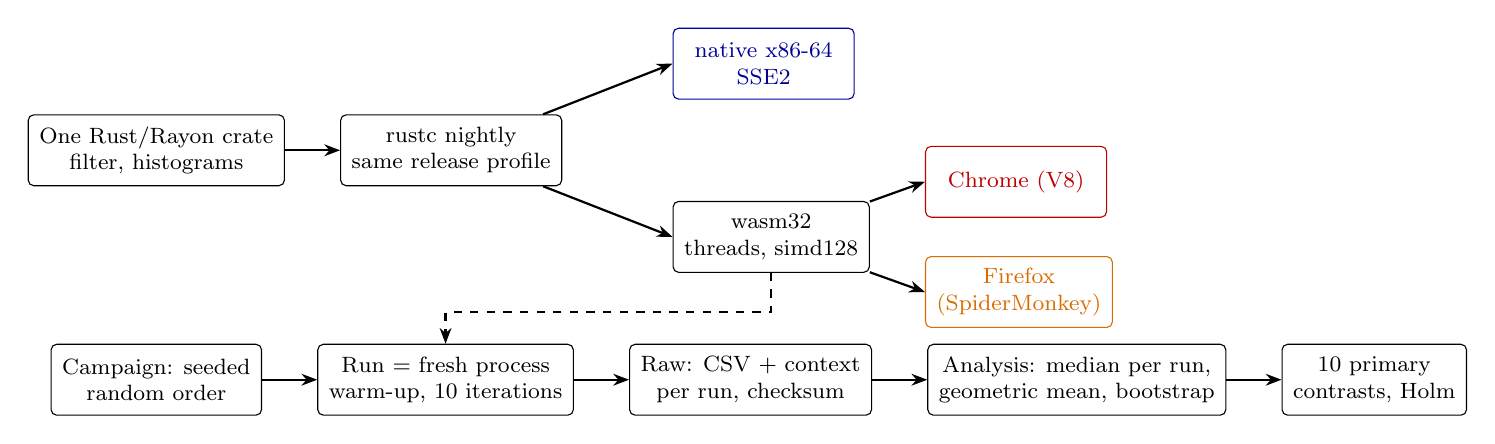
\begin{tikzpicture}[
  node distance=5mm and 7mm,
  box/.style={draw, rounded corners=2pt, align=center, font=\footnotesize, inner sep=4pt, minimum height=9mm},
  env/.style={box, minimum width=23mm},
  arr/.style={-{Stealth[length=2mm]}, thick}]
  \node[box] (src) {One Rust/Rayon crate\\filter, histograms};
  \node[box, right=of src] (rustc) {rustc nightly\\same release profile};
  \node[env, right=14mm of rustc, yshift=11mm, draw=native, text=native] (nat) {native x86-64\\SSE2};
  \node[env, right=14mm of rustc, yshift=-11mm] (wasm) {wasm32\\threads, simd128};
  \node[env, right=of wasm, yshift=7mm, draw=chrome, text=chrome] (chr) {Chrome (V8)};
  \node[env, right=of wasm, yshift=-7mm, draw=firefox, text=firefox] (ffx) {Firefox\\(SpiderMonkey)};
  \draw[arr] (src) -- (rustc);
  \draw[arr] (rustc) -- (nat.west);
  \draw[arr] (rustc) -- (wasm.west);
  \draw[arr] (wasm) -- (chr.west);
  \draw[arr] (wasm) -- (ffx.west);
  \node[box, below=20mm of src] (camp) {Campaign: seeded\\random order};
  \node[box, right=of camp] (run) {Run = fresh process\\warm-up, 10 iterations};
  \node[box, right=of run] (raw) {Raw: CSV + context\\per run, checksum};
  \node[box, right=of raw] (ana) {Analysis: median per run,\\geometric mean, bootstrap};
  \node[box, right=of ana] (res) {10 primary\\contrasts, Holm};
  \draw[arr] (camp) -- (run);
  \draw[arr] (run) -- (raw);
  \draw[arr] (raw) -- (ana);
  \draw[arr] (ana) -- (res);
  \draw[arr, dashed] (wasm.south) |- ($(run.north)+(0,4mm)$) -- (run.north);
\end{tikzpicture}
\caption{The study. Top: one source and one compiler give two artifacts and
three environments. Bottom: a campaign runs every configuration of the three
environments in one random order; each run is a fresh process that records
its times, its checksum and its context; the analysis is fixed before the
data.}
\Description{A flow from one Rust crate through the compiler to a native binary and a WASM module that runs in Chrome and Firefox, and a second flow from campaign to runs to raw data to analysis to contrasts.}
\label{fig:pipeline}
\end{figure}

Figure~\ref{fig:pipeline} is the whole design. One Rust crate holds the
workloads. The same compiler and release profile build a native x86-64
runner and a WASM module; the module runs in Chrome and in Firefox. A
campaign is a list of configurations (environment, workload, input, thread
count, repetition) shuffled once with a recorded seed, so native, Chrome and
Firefox runs are interleaved. Each run is one fresh process or one fresh
browser launch; it measures itself, checks its output against a checksum and
stores its times with the state of the machine. The analysis reads the runs,
never the iterations, as independent observations.

\subsection{Three builds}
\label{sec:builds-history}

The measured code was built three times, and the study was measured in full
twice. Code layout alone moves timings~\cite{mytkowicz2009}, so a rule holds
from the first build on: every campaign runs one tagged build, and no table,
figure or comparison combines runs of two builds.

\begin{description}[leftmargin=1.5em]
\item[v1.] The first build ran the main campaign and the first exploratory
ones. A review of the measured path on 2026-11-09 then found two asymmetries
that our own code had introduced into RQ2. The shared-counter histograms
indexed a table whose length the compiler did not know, so every pixel paid
a bounds check that the local control did not pay; and the final step of a
histogram (the reduce of the local variant, the read-back of the shared
counters) was timed in some variants and not in others.
\item[\code{measured/v2}.] The second build removed both asymmetries
(fixed-size counter tables; every variant times its final step), added
settings the next campaigns needed (passes per timed sample, a grain per
task, a second fork-join probe, the memory size) and nothing that optimizes.
Every campaign was run again on it. An audit of the finished study on
2026-11-20 found no reason to measure again, but listed what v2 could only
declare: the speedup had no sequential reference, the two histograms did not
build their tasks through the same code, the slow one-thread runs had no
established cause, the compiler tier that the campaigns measure was
inferred, and several explanations were hypotheses.
\item[\code{measured/v3}.] The third build turns those declared items into
measurements. It adds sequential versions of the kernels, sends the atomic
histogram through the same task-building code as the local one, and records
the memory size before the measured phase; the harness also records, per
run, the busy time of every measured CPU, and can run a browser with one
compiler only. No change is an optimization, and the code that counts is
the same machine code as in v2 (Section~\ref{sec:codegen}).
\end{description}

The results of v2 were known when v3 was designed, so v3 is a replication
with corrections, not a blind experiment. To keep the choice of the reported
build from following the numbers, the rule was written before any v3 run
existed: v3 is reported if, by 2026-11-27, its main campaign has every
planned run, no checksum conflict, and at least 10 runs left in every
configuration of the primary contrasts after the plan's exclusions;
otherwise v2 is reported and v3 is not used. The criteria read counts of
runs, never a time or a contrast. They were met on 2026-11-22: 5310 of 5310
runs, none failed, missing or excluded, no checksum conflict.

\paragraph{The replication agrees.} All ten primary decisions of v3 are
those of v2: the two contrasts not rejected in v2 are not rejected in v3
(Chrome on the filter, 0.996 in v3 and 0.990 in v2; Firefox at $k=1$, 1.010
and 0.994), and the other eight are rejected in both with effects of the
same sign. Every exploratory campaign of v2 has its twin on v3. This report
gives the v3 numbers only.

\section{Platform and Environment Control}
\label{sec:platform}

\begin{figure}[t]
\centering
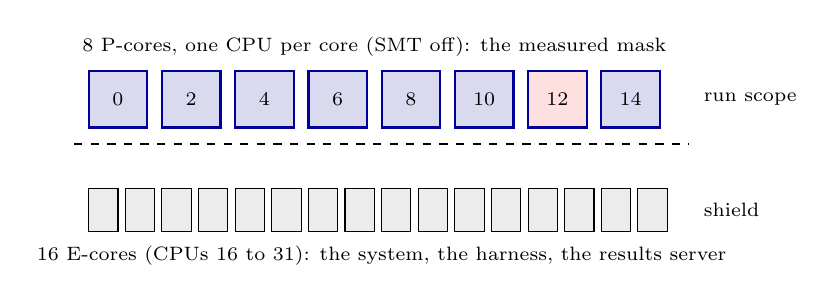
\begin{tikzpicture}[x=6.2mm,y=6mm,font=\scriptsize]
  \foreach \i/\c in {0/0,1/2,2/4,3/6,4/8,5/10,6/12,7/14} {
    \draw[fill=native!15, draw=native, thick] (\i*1.5,0) rectangle ++(1.2,1.2);
    \node at (\i*1.5+0.6,0.6) {\c};
  }
  \draw[fill=red!12, draw=native, thick] (9,0) rectangle ++(1.2,1.2);
  \node at (9.6,0.6) {12};
  \node[anchor=south] at (5.85,1.3) {8 P-cores, one CPU per core (SMT off): the measured mask};
  \foreach \i in {0,...,15} {
    \draw[fill=gray!15] (\i*0.75,-2.2) rectangle ++(0.6,0.9);
  }
  \node[anchor=north] at (6,-2.3) {16 E-cores (CPUs 16 to 31): the system, the harness, the results server};
  \draw[dashed] (-0.3,-0.35) -- (12.3,-0.35);
  \node[anchor=west] at (12.4,0.6) {run scope};
  \node[anchor=west] at (12.4,-1.75) {shield};
\end{tikzpicture}
\caption{The CPU layout during a measurement. A run is confined to the eight
P-cores by a systemd scope and a process-level mask; everything else is
confined to the E-cores. CPU 12 is the degraded core
(Section~\ref{sec:core}).}
\Description{Eight boxes for the P-core CPUs 0 to 14 and sixteen smaller boxes for the E-cores, separated by a dashed line.}
\label{fig:cores}
\end{figure}

\paragraph{Machine.} An Intel Core i9-14900KF on an ASUS ProArt Z790-CREATOR
WIFI (BIOS 3202), 64~GB of RAM, Ubuntu 26.04.1 LTS, kernel 7.0.0-43,
microcode 0x133. The CPU is hybrid: 8 P-cores with two hardware threads
each and 16 E-cores. The last-level cache is 36~MB.

\paragraph{P-cores only, one mask for all.} The study measures how the time
changes with $N$. If threads could land on either kind of core, the speed of
a thread would change with $N$ for reasons that have nothing to do with
WASM. The usual control, pinning each thread, is not available: a web page
cannot choose the core of a worker. So both sides get the same
process-level mask, the eight P-cores, and the kernel places threads inside
it (Figure~\ref{fig:cores}). A pilot confirmed the choice
(Section~\ref{sec:pilots}).

\paragraph{SMT off.} Linux numbers the two hardware threads of a P-core side
by side, so a mask such as \code{0-7} is four cores, not eight. SMT is off
for every session and the mask is \code{0,2,4,6,8,10,12,14}; every run
records the SMT state and the siblings of each masked CPU, and a run whose
mask has two CPUs on one core is rejected.

\paragraph{Turbo off, governor \code{performance}.} With turbo on, one busy
core runs at a higher clock than eight busy ones, so $T_1$ would be measured
at a higher frequency than $T_8$ and the speedup would be deflated for a
reason unrelated to parallelism. With turbo off the P-cores run at their
3.2~GHz base clock (the recorded maximum of every measured CPU is
3\,200\,000~kHz).

\paragraph{Shield.} A mask keeps the run on the P-cores; it does not keep
anything else off them. On a hybrid CPU the scheduler even prefers the
P-cores. The system, user and init slices are therefore confined to the
E-cores at run time, the harness and the results server pin themselves
there, and each run is started in its own systemd scope whose allowed CPUs
are the mask. What the shield cannot stop (per-CPU kernel threads,
interrupts) is measured: every run records the busy time of the measured
CPUs minus its own CPU time, the \emph{foreign CPU time}, and a run above a
threshold fixed from pilot data is excluded (Section~\ref{sec:pilots}).

\paragraph{Quiet mode.} Before a campaign the desktop session and bursty
services (containers, package timers, snaps) are stopped, because they share
the last-level cache and the memory bandwidth with the measured cores even
when they run on other CPUs; the machine does not sleep during a campaign.

\paragraph{Checked before every start, recorded with every run.} None of
these settings survives a reboot. A campaign refuses to start, and to
resume, unless turbo is off, the governor is \code{performance} on every
measured CPU, SMT is off, the mask is exactly one CPU per P-core, the shield
holds and the pinned browser versions are the installed ones. Each run
stores the commit, the CPU model, kernel, governor, turbo and SMT state, the
mask, the browser version, the launch command, the order seed and position,
the foreign CPU time, the processes found outside its scope, the load
average, and for every measured CPU its busy time. \emph{Strict validation}
rejects a run in which any of them is missing or wrong. Since v3 the host
state that the setup leaves alone is recorded too: transparent huge pages
(\code{madvise}), the kernel command line, the mitigations, the idle driver
and its C-states, the firmware and the memory size.

\subsection{The degraded core}
\label{sec:core}

One P-core of the machine is degraded: the seventh, CPU 12 of the mask.
Before the v3 build every P-core was checked, with the rule fixed in
advance: the eight cores stay whatever times the check shows, and a core
leaves the mask only on a wrong checksum or a crash.

\begin{itemize}[leftmargin=1.5em]
\item \emph{On the machine as found it fails.} With turbo on, SMT on, the
governor \code{powersave} and no shield, a test suite pinned to that core
crashed with a segmentation fault in 17 of 18 runs, and in 0 of 28 runs
pinned elsewhere.
\item \emph{On the prepared machine it does not.} After the setup the same
tests passed 30 of 30 times on CPU 12. The setup changes four things
together, so the check does not say which one matters; turbo is the likely
one, since it is what lets the core run above 3.2~GHz.
\item \emph{On the prepared machine it is as fast as the others}
(Table~\ref{tab:core-check}): the native filter at one thread pinned to one
core at a time gives 22.41 to 22.53~ms on every core, 22.44 on CPU 12, the
right checksum in all 80 runs, and no iteration above 22.9~ms among 800.
\end{itemize}

\begin{table}[htbp]
\caption{Per-core check on the prepared machine: the native filter at one
thread, 8192$\times$8192, pinned to one P-core at a time, 10 runs per core
in rotating order (a check, not a result).}
\label{tab:core-check}
\centering\small
\begin{tabular}{lrrrrrrrr}
\toprule
CPU & 0 & 2 & 4 & 6 & 8 & 10 & 12 & 14 \\
\midrule
Median (ms) & 22.53 & 22.41 & 22.43 & 22.42 & 22.42 & 22.53 & 22.44 & 22.44 \\
Against all runs & 1.004 & 0.999 & 0.999 & 0.999 & 0.999 & 1.004 & 1.000 & 1.000 \\
\bottomrule
\end{tabular}
\end{table}

Three decisions followed. CPU 12 stays in the mask. The measured build is
made on the prepared machine and twice from scratch, tagged only if the
digests agree, because on the unprepared machine a process that is not
pinned can land on the failing core, the compiler included, and a failing
core can compute wrongly without crashing. And tests and analysis on this
machine run after the setup, or pinned away from that core. The last rule
was needed once: after the machine was restored for the hybrid campaign, a
table command stopped with a \code{TypeError} raised inside Python's own
\code{statistics} module on data that the same command reads without error,
a wrong computation with no crash and no kernel log entry. The tables were
written pinned away from the core, and the continuous integration now
regenerates every table on another machine and compares it with the
committed one.

The main campaign adds what a pinned check cannot. With one thread the
kernel put the work on CPU 12 or 14 (Table~\ref{tab:core-split}); the
native filter ran mostly on CPU 12 in 9 of its 30 runs, with a median
1.0003 times that of the configuration. The slow one-thread runs that the
earlier build showed (five filter runs 1.21 times their configuration's
median) did not come back: no native filter run at one thread is above
1.005 times the median.

\begin{table}[htbp]
\caption{One-thread filter runs of the main campaign split by the CPU with the most busy time: runs, their median and slowest run over the configuration's median, and that CPU's share of the run's busy time. CPU 12 is the degraded core.}\label{tab:core-split}
\centering\small
\begin{tabular}{llrrrrr}
\toprule
Environment & Workload & CPU & Runs & Median & Max & Busy share \\
\midrule
Chrome & filter & 12 & 12 & 1.0026 & 1.0144 & 0.643 \\
Chrome & filter & 14 & 18 & 0.9986 & 1.0189 & 0.595 \\
Chrome & filter-seq & 12 & 16 & 1.0043 & 1.0190 & 0.811 \\
Chrome & filter-seq & 14 & 14 & 0.9938 & 1.0216 & 0.807 \\
Firefox & filter & 12 & 11 & 1.0020 & 1.0426 & 0.471 \\
Firefox & filter & 14 & 19 & 0.9997 & 1.0622 & 0.485 \\
Firefox & filter-seq & 12 & 12 & 1.0052 & 1.0525 & 0.562 \\
Firefox & filter-seq & 14 & 18 & 0.9997 & 1.0352 & 0.559 \\
Native & filter & 12 & 9 & 1.0003 & 1.0029 & 0.801 \\
Native & filter & 14 & 21 & 0.9997 & 1.0049 & 0.706 \\
Native & filter-seq & 12 & 22 & 1.0000 & 1.0017 & 0.990 \\
Native & filter-seq & 14 & 8 & 1.0001 & 1.0016 & 0.990 \\
\bottomrule
\end{tabular}
\end{table}


\section{Builds}
\label{sec:builds}

\paragraph{One source, one compiler, one profile.} The crate is compiled by
a pinned nightly Rust (\code{nightly-2026-10-03}, rustc 1.101.0) with
\code{lto = "fat"}, one codegen unit and \code{panic = "abort"}, for two
targets: x86-64 with its baseline instruction set (SSE2; no
\code{target-cpu=native} anywhere) and \code{wasm32} with the target
features \code{+atomics}, \code{+bulk-memory}, \code{+mutable-globals} and
\code{+simd128}. WASM threads need the standard library rebuilt with
atomics (\code{-Z build-std}), which exists only on nightly; a fixed date
makes the compiler, the library and LLVM the same for both targets. The
crates are locked: Rayon 1.12.0, rayon-core 1.13.0, wasm-bindgen 0.2.129,
wasm-bindgen-rayon 1.3.0. No \code{wasm-opt} pass rewrites the module.

\paragraph{128-bit SIMD on both sides, verified on the artifacts.} WASM has
128-bit SIMD only, so the native build is held to SSE2, also 128-bit. The
code has no explicit SIMD: the vector instructions come from the compiler's
auto-vectorization, so parity is a property to test, not to assume. The
filter's interior loop is a separate, never-inlined function
(\code{blur\_interior}) so that it keeps a symbol in the final binaries, and
the continuous integration disassembles the final native binary and the
final WASM module on every change and requires packed 16-bit arithmetic in
that function on both. With whole-program optimization the vectorization
happens at the final link, so checking a library's assembly would mislead.

\paragraph{What differs below the shared source.} ``The same code'' is
claimed for the crate, not for the layers below it, which are the
environment under study:
\begin{itemize}[leftmargin=1.5em]
\item \emph{Flags.} The target features and link arguments exist only for
WASM; a native run records empty extra flags.
\item \emph{Standard library.} Native links the prebuilt library; WASM
rebuilds it under the project's profile.
\item \emph{Locks inside Rayon.} \code{wasm-bindgen-rayon} enables a Rayon
feature that replaces its mutex and condition variable with spin-based ones,
on WASM only.
\item \emph{Idle threads.} On \code{wasm32} with atomics the standard
library's \code{yield\_now} does nothing, so the yield rounds of Rayon's
idle loop spin without giving up the CPU where native code calls
\code{sched\_yield}; to sleep, a WASM worker waits in
\code{memory.atomic.wait32} and a native worker on a futex.
\item \emph{A second compiler.} The engines compile the WASM for the host
CPU, so they may use encodings newer than the SSE2 the native build is held
to. The vector width is fixed at 128 bits, not the instruction set
(Section~\ref{sec:engine-code}).
\end{itemize}
The idle and wake path is inside every timed iteration of a parallel
region. It is the leading candidate for the browsers' larger fork-join cost
(Section~\ref{sec:forkjoin}); no experiment here isolates it.

\paragraph{The build is reproducible and made twice.} On the prepared
machine the build stage runs the tests and then builds twice from scratch;
the tag \code{measured/v3} (commit \code{ac65af6a}) was made only because
both builds gave the same SHA-256 digests for the native runner
(\code{525707de...}), the WASM module (\code{38787129...}) and the
JavaScript glue. Every campaign records the digests of the binaries it ran,
and refuses to resume with another commit, artifact or browser version.

\subsection{What changed in v3, and what the compiler made of it}
\label{sec:codegen}

A change in the measured path is allowed only with a record of why, and is
checked by a script that builds the base and the new source at the same
path and compares the normalized instructions of every hot function. Before
any change, the source of this repository gave the machine code of v2:
native 88 of 88 hot functions identical, WASM 87 of 87.

\begin{enumerate}[leftmargin=2em]
\item \emph{Every shared-counter histogram builds its tasks through the
grain control}, as the local histogram and the filter do. With Rayon's
adaptive split this calls the library's default, and a test counts the
tasks with and without the call on a pool of one thread: the counts are
equal. The script reports the \code{run} of the three histograms as
changed (it now reads the grain) and the Rayon functions instantiated for
them as renamed. The counting loops were therefore compared by hand, from
just before the first atomic add to just after the last: natively the loop
of 37 instructions is identical (\code{movzbl; shl \$7; lock incq} eight
times per turn, the same registers), and in WASM the loop of 127
instructions is identical. The code that counts is unchanged; the code that
splits now is the same for every histogram.
\item \emph{Sequential references.} Two workloads with no Rayon call, at
one thread only: one loop over the rows that calls \code{blur\_interior},
and one loop that counts into one plain table. Adding a workload can change
another one: the first draft called the parallel filter's row function,
which had one caller and was inlined; with a second caller the compiler
kept it as a call and the machine code of the parallel filter changed,
though its source had not. The sequential filter therefore has its own copy
of the row and edge handling and shares only \code{blur\_interior}; a test
keeps its output equal to the parallel filter's. With both changes, the
parallel filter's task function, \code{blur\_interior}, the local histogram
and the checksum functions are identical to v2 in every variant.
\item \emph{The memory size before the measured phase is written.} It was
already sampled, for the check that fails a WASM run whose memory grows
while it is measured; no new sample is taken. A native filter run shows
what it is for: 69.7~MB before the warm-up, 136.8~MB before the first
measured iteration, 136.8~MB after the last. The 64~MiB of the output
buffer are first touched in the warm-up.
\end{enumerate}

The golden checksums are unchanged. Because the split code changed, the
times of v3 are never compared number by number with those of v2; the
exploratory twin campaigns still show, as a consistency observation, that
the cells whose task code changed kept their times (the private histogram
within 0.2\% of v2 at eight threads, Section~\ref{sec:extras}).

\section{Workloads}
\label{sec:workloads}

Every workload implements one interface: \code{prepare} (untimed, before
each iteration), \code{run} (the timed work) and \code{checksum} (untimed).
Buffers are allocated in the constructor: WASM's default allocator takes a
global lock, so an allocation inside the timed region would add a
synchronization cost that native code does not have.

\paragraph{Inputs.} Images are 8192$\times$8192 single-channel \code{u8}
pixels (67 megapixels, 64~MiB), generated outside the timed region by a
SplitMix64 generator implemented in the crate and seeded with a fixed
constant, so the pixels are bit-identical in every environment. The
\emph{noise} input takes uniform values 0 to 255. The \emph{few-colours}
input takes $k$ values evenly spaced over 0 to 255, each pixel picking one
uniformly. Every run records the seed, $k$ and a fingerprint of the input.

\paragraph{Gaussian filter: no synchronization.} A $3\times3$ kernel
$[1\,2\,1; 2\,4\,2; 1\,2\,1]/16$ in integer arithmetic with rounding, edges
clamped. Rows are processed in parallel (\code{par\_chunks\_mut} over the
output rows): each task writes its own row and reads the shared, immutable
source, so threads never coordinate, and any loss of speedup comes from the
environment. Integer arithmetic gives the same result on every target and
thread count, where floating point could differ with SIMD. The interior
loop works on 16-bit values (the largest sum, $16\times255$, fits) and is
the function whose vectorization is checked. The filter reads one 64~MiB
image and writes another.

\paragraph{Histogram: two variants with the same result.} The histogram
counts the pixels of each value into 256 bins.
\begin{itemize}[leftmargin=1.5em]
\item \emph{Atomic}: all threads increment 256 shared \code{AtomicU64}
counters (\code{fetch\_add(1)}). Each counter is padded to its own 128-byte
block, so that two different counters never share a cache line: what is
measured is true sharing, not false sharing. 128 and not 64 bytes because
the adjacent-line prefetcher fetches 64-byte lines in pairs. The counters
are reset in \code{prepare}, outside the timed region.
\item \emph{Local}, the lock-free control: each task counts into its own
plain table and the tables are merged at the end (\code{fold} and
\code{reduce}). No write is shared.
\end{itemize}
Both split the pixels into 64~KiB chunks and build their tasks through the
same code, both index fixed-size tables (no bounds check per pixel), and
both time their final step (the reduce, or the read-back of the shared
counters). They differ in how the counts are combined, which is the factor
of RQ2. The memory ordering asked for is \code{Relaxed}; it makes no
difference on these targets, since x86 locked instructions are full
barriers and WASM atomics are always sequentially consistent.

\paragraph{Contention is set by $k$.} The histograms run on the few-colours
input with $k \in \{1, 4, 16, 256\}$: the updates are spread over $k$
counters, from every pixel on one counter to a uniform spread over all 256.
The first design called the two ends ``high'' and ``low'' contention; a
review before any data replaced the names, because with 256 counters and
eight threads most increments still find their line modified by another
core. What $k$ changes is how the contention is spread. $k$ also changes
the control: with few values the local histogram increments the same
address again and again, a chain in which each increment waits for the
previous store (store-to-load forwarding), with no synchronization
involved. The RQ2 metric is built so that this effect of the input cancels
(Section~\ref{sec:plan}).

\paragraph{Padding, checked.} A pilot compared 64-byte with 128-byte padding
natively (10 runs per cell): every one-thread cell within 0.6\%, and at
eight threads ratios of 0.99 to 1.02 with intervals that reach 7\% either
way at $k=1$; no difference was detected and 128 was kept as the safer
choice. A \code{perf c2c} run in Chrome at $k=16$ showed 16 contended lines
0x800 bytes apart (16 bins of 128 bytes), each accessed at one offset: the
alignment holds inside WASM linear memory. The 64-byte variant was later
removed from the code.

\paragraph{Checksums.} Every workload hashes its output (FNV-1a, which
depends on the position of every byte) outside the timed region. The
checksum of a run must equal that of every other run of the same workload
and input, whatever the environment and the thread count; a conflict stops
the analysis. Golden checksums are pinned in the tests, and the continuous
integration runs every workload in both browsers and compares checksums and
input fingerprints with the native run. No campaign of v3 has a conflict.

\paragraph{Sequential references.} \code{filter-seq} and \code{hist-seq} are
the same kernels called from a plain loop with no Rayon, at one thread
only. They answer whether a pool of one thread is a fair baseline for the
speedup (Section~\ref{sec:sequential}).

\paragraph{Variants of the exploratory campaigns.} \emph{Private} atomics:
every thread increments its own padded table of atomic counters, so the
atomic instruction is paid and no line is shared; with local and shared it
forms a ladder that separates the cost of the instruction from the cost of
contention. \emph{Packed} atomics: the 256 shared counters are contiguous,
eight per 64-byte line, the false-sharing level next to the padded one.
\emph{Sorts}: Rayon's stable parallel sort, a merge sort that allocates its
buffer and so exercises WASM's allocator, and the unstable in-place sort as
its control, on the pixels read as 32-bit keys.

\section{Harness and Run Protocol}
\label{sec:harness}

\paragraph{No automation framework.} A framework that drives the browser
(Puppeteer, Playwright, a debugging protocol) attaches code and threads to
the process being measured. The harness instead launches the browser binary
like a user would, with the page URL carrying the configuration, and the
page posts its results to a local server. The server also sends the COOP
and COEP headers that shared memory needs. Nothing is attached to the
browser while it measures.

\paragraph{A browser run.} The launcher creates an empty temporary profile,
starts the browser headless in its own process group, inside the run's
scope and mask, and waits for the result file. The page waits a fixed start
delay, creates the coordinating worker (the main thread cannot block),
which instantiates the module, creates the thread pool and runs the
measurement, and posts the rows and the page's metadata. The launcher then
stops the scope, signals the whole process group so that no renderer
survives into the next run, and deletes the profile. Background work is
turned off symmetrically in both browsers (updates, telemetry, safe
browsing, remote settings, prefetching; background throttling in Chrome).
A run ends as done, timed out or exited without a result; a failed run is
recorded, not retried silently, and the campaign reports a failure rate.

\paragraph{A native run} goes through a wrapper that starts the runner in
the same kind of scope with the same mask and writes the same pair of files
(the rows and the context).

\begin{figure}[t]
\centering
\resizebox{\linewidth}{!}{%
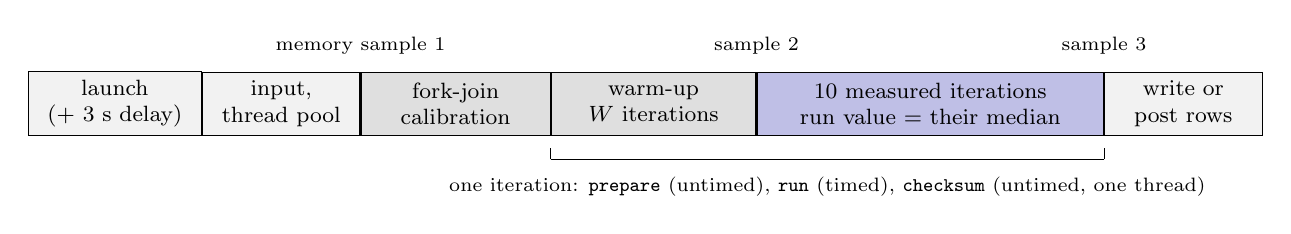
\begin{tikzpicture}[font=\footnotesize, node distance=0pt,
  ph/.style={draw, minimum height=8mm, inner sep=3pt, align=center}]
  \node[ph, fill=gray!10, minimum width=22mm] (launch) {launch\\(+ 3 s delay)};
  \node[ph, fill=gray!10, minimum width=20mm, right=of launch] (pool) {input,\\thread pool};
  \node[ph, fill=gray!25, minimum width=24mm, right=of pool] (cal) {fork-join\\calibration};
  \node[ph, fill=gray!25, minimum width=26mm, right=of cal] (warm) {warm-up\\$W$ iterations};
  \node[ph, fill=native!25, minimum width=44mm, right=of warm] (meas) {10 measured iterations\\run value = their median};
  \node[ph, fill=gray!10, minimum width=20mm, right=of meas] (post) {write or\\post rows};
  \draw[decorate] ($(warm.south west)+(0,-3mm)$) -- node[below, font=\scriptsize, yshift=-1mm] {one iteration: \code{prepare} (untimed), \code{run} (timed), \code{checksum} (untimed, one thread)} ($(meas.south east)+(0,-3mm)$);
  \draw ($(warm.south west)+(0,-3mm)$) -- ++(0,1.5mm);
  \draw ($(meas.south east)+(0,-3mm)$) -- ++(0,1.5mm);
  \node[font=\scriptsize, above=1mm of pool.north east, anchor=south] {memory sample 1};
  \node[font=\scriptsize, above=1mm of meas.north west, anchor=south] {sample 2};
  \node[font=\scriptsize, above=1mm of meas.north east, anchor=south] {sample 3};
\end{tikzpicture}}
\caption{The layout of one run, the same in the three environments. Only
the measured iterations enter the analysis; the calibration is reported
separately and nothing is subtracted from the times.}
\Description{A timeline of a run: launch, input and thread pool, fork-join calibration, warm-up iterations, ten measured iterations, and writing the rows.}
\label{fig:run}
\end{figure}

\paragraph{The layout of a run} is shared code, the same in the three
environments (Figure~\ref{fig:run}). The input is generated and the pool of
$N$ threads is created first. Then the \emph{fork-join calibration} times
empty parallel regions, 20 samples each of two probes: an empty
\code{broadcast}, which every worker must run (a barrier), and an empty
parallel iterator (ordinary optional parallelism); each probe is timed warm
(back to back, workers spinning) and cold (after a pause at least as long
as the workload's checksum, so the workers are asleep, as they are before a
measured iteration). Then come $W$ warm-up iterations and 10 measured
ones. In each iteration only \code{run} is between the two clock reads.
Every iteration is called from outside the pool, natively from the main
thread and in WASM from the coordinating worker, as an application calls a
parallel library. The memory size (the native resident set, the WASM linear
memory) is recorded before the warm-up, before the first measured iteration
and after the last; a WASM run whose memory grows during the measured phase
fails. The clock is \code{performance.now()} in the browsers, with a
resolution measured in every run: 5~\textmu s in Chrome, 20~\textmu s in
Firefox.

\paragraph{What a run writes.} One CSV with a row per iteration (phase,
index, nanoseconds, checksum, and the settings of the run) and one JSON
with the context of Section~\ref{sec:platform}. The run identifier is not
stored in the rows; the analysis joins it, so a file cannot be filed under
the wrong run.

\paragraph{The orchestrator.} A campaign is a JSON specification holding
every parameter: environments, workloads with their input, $k$ and warm-up,
thread counts, repetitions, image size, iterations, calibration samples,
masks, start delay and timeout. Unknown keys are rejected. The orchestrator
builds every combination, shuffles the whole list once with the recorded
seed and runs it in that order, so that a slow drift of the machine
(temperature, background activity) is spread over the environments instead
of lining up with one. Before the plan, each browser is launched once and
discarded, because the first launch on a machine is slow. A campaign that
is stopped resumes: finished runs are skipped and the order is the same. It
refuses to continue with another specification, commit, artifact digest or
browser version, so one campaign never mixes builds. During a campaign
nothing else is started on the machine.

\paragraph{The session of a build.} Measuring a build is a sequence of
numbered, resumable stages, each writing its log:
\begin{enumerate}[leftmargin=2em]
\item \emph{Preflight}: the host state as found, the environment set up and
checked, the tests, a tiny copy of every campaign to exercise the pipeline
end to end, and the per-core check of Section~\ref{sec:core}.
\item \emph{Build}: the tests, two builds from scratch, the digests, the
tag.
\item \emph{Gate}: a short campaign on the cells whose code changed, with
criteria fixed in advance (Section~\ref{sec:gate}).
\item \emph{Main campaign}, then the exploratory ones, in an order chosen so
that what is dropped for lack of time is dropped from the end.
\item \emph{Results}: every table and figure, then a check that
regenerating them changes nothing.
\end{enumerate}

\subsection{The gate}
\label{sec:gate}

The gate ran the cells whose code changed (both histograms at $k=1$ and
256, the sequential workloads) and the filter as a control, at $N=1$ and 8
in the three environments, 3 runs each at the real size: 135 runs. It
passes when, in every cell, the checksums agree across environments and
thread counts, every timed sample is at least 100 clock ticks, and the
median of the first three measured iterations is within 5\% of the median
of the last three. Three runs only catch a gross failure, such as a warm-up
that no longer covers a tier change. How a failure is read was fixed
beforehand too: the gate is run once more, whole, with another seed, and
the same cell failing twice stops the session for a recorded decision.

Both gates ran without a failed or excluded run and passed the first two
criteria; 44 of 45 cells passed the third, and the same cell failed both
times: Firefox, local histogram, $k=1$, $N=8$, with ratios of 1.052 and
1.077. In every one of its six runs, one or two of the first three measured
iterations take 21 to 22~ms and the others 19.7~ms; the 71 warm-up
iterations before them show nothing of the kind. The run value is a median
of ten iterations, which one or two slow ones do not move: it is 1.000 to
1.0015 times the value taken from the last seven iterations alone. The
decision, recorded before the main campaign started: the campaigns go ahead
with every parameter unchanged, the gate stays recorded as failed on one
criterion in one cell, and the cell is declared with its measured effect of
about 0.1\%. Changing the measurement after seeing data (dropping the first
iterations, lengthening the warm-up) was the alternative rejected. The tier
campaign later showed that these slow iterations come with the optimizing
compiler's code (27 of 30 runs as shipped and with the optimizing compiler
only, 1 of 30 with the baseline compiler only); what they are is not known.

\section{Pilot Decisions}
\label{sec:pilots}

The analysis plan left a few values to pilot data. Each was fixed before
the first campaign from a pilot run on the measuring machine, and is listed
here with the number behind it (Table~\ref{tab:pilots}). Pilot numbers are
evidence for a decision; none is a result, and none is mixed with the
campaigns. The pilots ran on the first build.

\begin{table}[htbp]
\caption{The values fixed from pilots, and the evidence for each. All
numbers in this table are pilot numbers, not results.}
\label{tab:pilots}
\centering\footnotesize
\begin{tabular}{p{0.2\linewidth}p{0.2\linewidth}p{0.5\linewidth}}
\toprule
Decision & Value & Evidence from the pilot \\
\midrule
Image size & 8192$\times$8192 & Smallest size at which the fastest browser cell at $N=8$ is over 100 clock ticks in both browsers (Firefox 213 ticks, Chrome 802) \\
Clock factor & 100 ticks & A factor of 1000 would need images above 20\,000$^2$ in Firefox; 100 caps the quantization of one sample at 1\% \\
Warm-up $W$ & 5 to 71, per workload & 1.5 times the largest warm-up observed in any environment, thread count and run of 100-iteration runs \\
Thread counts & 1, 2, 4, 6, 7, 8 & $N=7$ locates where a knee at the last thread would start \\
Mask & 8 P-cores & With the E-cores added, $N=8$ runs were slower in 5 of 6 cells (3 to 19\%) and several times more variable \\
Display & headless & Headful over headless within 0.3\% in four cells, intervals within 1.2\% \\
Start delay & 3 s & Without it, Firefox's local histogram at $N=8$ was 1.32 times slower (ratio 0.756 [0.721, 0.790]) with bursts in 3 of 10 runs \\
Runs & 30 per cell & 99.5\% half-widths under 1\% for RQ1 and 1.1 to 7.5\% for RQ2 \\
Iterations & 10 per run & More iterations do not improve the agreement of the per-run median (93 to 96\% within 2\% for every count tried) \\
Foreign CPU threshold & 0.25 s & Twice the largest value of 1638 pilot runs (0.125 s) \\
Chrome build & Chrome for Testing & Within 1.3\% of the branded stable Chrome of the same version in four cells \\
Padding & 128 bytes & No difference detected against 64 bytes (Section~\ref{sec:workloads}) \\
\bottomrule
\end{tabular}
\end{table}

\paragraph{Image size and the clock.} A browser clock that is coarse
compared with an iteration makes the measured time mostly quantization
error. The size sweep measured the resolution of \code{performance.now()}
in every browser run, 5~\textmu s in Chrome and 20~\textmu s in Firefox, and
the fastest configuration at $N=8$ in clock ticks: 24, 68, 213 and 322 in
Firefox at sides of 2048, 4096, 8192 and 10\,240. The plan started with a
factor of 1000, which is out of reach at any usable size; the factor became
100, a warning and not an exclusion, and the image 8192$\times$8192, the
smallest size that clears it with a margin of two in Firefox. The sweep
also showed, with 3 runs and no intervals, that the gap between the
environments grows as the image shrinks (filter speedup at $N=8$ of 4.91
natively against 3.45 in Chrome at 2048$^2$, 6.68 against 6.61 at
8192$^2$), which is what the cutoff campaigns later measured properly
(Section~\ref{sec:cutoff}).

\paragraph{Warm-up.} Every workload ran with no warm-up and 100 measured
iterations at $N=1$ and 8. The first iteration is the most expensive
everywhere, natively too (the filter's first iteration takes five times the
steady state at $N=8$: the first write to the output buffer). Most cells
are steady after two or three iterations. The rule: a run's observed
warm-up is the first iteration whose next window of 10 has its median
within a tolerance of the steady state, the tolerance being the larger of
2\% and 1.5 times the largest window deviation inside the steady state, so
that noise is not read as warm-up; a workload's $W$ is 1.5 times the
largest observed value over environments, thread counts and runs, at least
5, and \emph{the same in every environment}. The values: 15 for the filter;
5 for the atomic histogram at every $k$; 71, 21, 15 and 15 for the local
histogram at $k=1$, 4, 16 and 256. The 71 comes from Firefox's local
histogram at $k=1$, which runs about 15\% slower for its first 26 to 47
iterations at $N=8$. A single $W$ of 71 for everything would have cost
about 20 more hours, spent on atomic iterations that show no warm-up.

\paragraph{Thread counts and oversubscription.} A browser runs threads of
its own. At $N=8$ the workers plus those threads may ask for more than the
eight cores of the mask, and the slowdown would look like poor scaling. The
first thread pilot showed a knee in Firefox's local histogram at $N=7$ and
8. The start-delay pilot then removed it: with a 3~s delay no browser shows
a knee. The knee most likely came from Firefox's start-up work competing
with eight workers, not from its threads during the measurement.
Oversubscription stays a possible, much smaller threat, and $N=7$ stays in
the design to show where a knee would start.

\paragraph{The mask, and the first pitfall.} The pilot that compared the
P-core mask with all cores found a problem before it found a result: a
sampler of every thread's allowed CPUs showed Chrome's browser process
outside the mask (Section~\ref{sec:problems}). With that fixed, runs at
$N=1$ agree within 1\% between the masks, and at $N=8$ the wider mask is
slower in 5 of 6 cells, by 3\% (Chrome filter) to 19\% (native local
histogram), with run-to-run variation growing from 0.9\% to 7.2\% for the
native filter: the workers share the cores with the system and land on
slower cores.

\paragraph{Headless.} The rule was fixed before measuring: run headless if
the 95\% interval of headful over headless includes 1 and the ratio is
within 2\%. In the filter and the local histogram at $N=8$, the four ratios
are 0.998 to 1.003 and every interval includes 1.

\paragraph{Start delay.} A freshly launched browser keeps doing start-up
work after the page loads, inside the same mask as the measurement. With no
delay, Firefox's local histogram at $k=16$ and $N=8$ took 5.89~ms against
4.46~ms with a 3~s delay, and its within-run spread (slowest over fastest
iteration) fell from 1.37 to 1.03; the other three cells did not move. A
6~s delay changed the medians by at most 1.3\% against 3~s. Native runs
have no delay, a known asymmetry: it affects $T_1$ and $T_N$ of an
environment alike.

\paragraph{Runs and iterations.} Thirty runs of every cell the primary
contrasts need were subsampled to see how the 99.5\% intervals narrow: with
30 runs the half-width is under 1\% for RQ1 and 1.1\% to 7.5\% for RQ2, the
widest being Chrome at $k=1$. A 5\% target everywhere would need about 60
runs; against RQ2 effects of a factor of two, a few percent is small. Two
thresholds proposed before the pilot (a 5\% half-width, a 1\% agreement of
the per-run median) were dropped after seeing its data, and the achieved
values are reported instead.

\paragraph{Chrome for Testing.} The pinned Chrome is Google's build for
testing, chosen because a fixed version can be downloaded later. Against
the branded stable Chrome of the same version, the filter and the atomic
histogram differ by at most 1.3\% (one interval, the filter at $N=8$,
excludes 1: [1.005, 1.020]), and two versions of the testing build differ
by at most 0.6\%. The comparison ran one build after the other, so a 1\%
effect of the build cannot be told from drift.

\section{Analysis Plan}
\label{sec:plan}

Choosing the statistics after seeing the data invites picking the one that
gives the nicest answer. The plan was written, committed and tagged before
any campaign data; later changes are dated amendments with their reason. It
is eight decisions.

\begin{description}[leftmargin=2.5em]
\item[Unit.] The run, one fresh process. Iterations inside a run are not
independent observations (they share the process's memory layout, its
compiled code and its thread placement), so treating them as such would be
pseudo-replication~\cite{georges2007,kalibera2013}. Run times are positive
and right-skewed and the questions are about ratios, so the analysis works
on log times and reports ratios.
\item[D1, per run.] The median of its 10 measured iterations.
\item[D2, per configuration.] A configuration is (environment, workload,
input, $k$, $N$). Its central value $T$ is the geometric mean of its 30 run
values. Speedup is $T(1)/T(N)$ within the same environment.
\item[D3, intervals.] Percentile bootstrap, 10\,000 resamples, fixed seed.
Runs are resampled, never iterations, and groups that are different
processes ($N=1$ and $N$; atomic and local; native and browser) are
resampled independently, since they are not paired.
\item[D4, RQ1.] The ratio of speedups $S(\mathrm{browser})/S(\mathrm{native})$
for each browser, workload and $N$; 1 means the browser scales like native.
\item[D5, RQ2.] For each environment $e$, $r(e,k,N) = \log T_{\mathrm{atomic}}
- \log T_{\mathrm{local}}$: how much slower the shared atomics are than the
lock-free control on the same input. The estimand is the interaction
$\Delta r = r(\mathrm{browser}) - r(\mathrm{native})$ at the same $k$ and
$N$, a difference of differences. Comparing within one input is what
removes the input's own effect on both variants.
\item[D6, effect sizes.] The ratios themselves: the speedup ratio for RQ1
and $\exp(\Delta r)$ for RQ2, the relative cost of the atomic variant in
the browser over the same relative cost natively.
\item[D7, exclusions.] No statistical outlier removal. Only three exclusions
exist, decided in advance and counted: failed runs, runs that fail strict
validation, and runs whose foreign CPU time is above 0.25~s.
\item[D8, multiple comparisons.] The \emph{primary family} has ten
contrasts, all at $N=8$: $\Delta r$ for $k \in \{1,4,16,256\}$ and both
browsers (eight), and the filter's log speedup ratio for both browsers
(two). Each has a two-sided bootstrap $p$-value, twice the smaller share of
bootstrap estimates on one side of zero, floored at $1/10\,000$. The
decision is Holm's procedure at a family-wise $\alpha=0.05$. Primary
contrasts are shown with Bonferroni 99.5\% intervals, which hold
simultaneously for the family. Everything else is exploratory: uncorrected
95\% intervals, labelled as such.
\end{description}

\paragraph{Why these choices.} Intervals on ratios show the size of an
effect and its uncertainty together, which a bare test does not. The
bootstrap makes no assumption about the shape of the run times. The
geometric mean is the natural centre for quantities compared by ratio. A
small primary family, fixed in advance, keeps the correction for multiple
comparisons from being diluted by the hundreds of descriptive cells.

\paragraph{Amendments.} Two were made before any data: every scaling
comparison is read next to the absolute time ratio
$T(\mathrm{browser},N)/T(\mathrm{native},N)$, because a relative speedup can
look better only because its baseline is slow~\cite{hoefler2015}; and a
configuration whose run value is under 100 clock ticks is flagged. One was
made after the first campaign's primary results existed, and is labelled as
such: a \emph{robustness check} that tests each primary contrast with
Mann-Whitney $U$~\cite{mann1947} and Cliff's $\delta$ on per-run ratios
($\log(T_1/T_N)$ for RQ1, $\log(T_{\mathrm{atomic}}/T_{\mathrm{local}})$ for
RQ2), Holm-adjusted. The two runs of a ratio are separate processes, paired
by repetition index, so the check is repeated over 1000 random re-pairings.
The bootstrap decisions stay the reported ones; a disagreement would be
reported as not robust.

\paragraph{Sensitivity checks.} The plan names three: the per-run mean
instead of the median, the median across runs instead of the geometric
mean, and no exclusion by foreign CPU time. A conclusion that changes under
one of them is reported as not robust.

\paragraph{The data check.} Before any analysis a report counts the runs
done, missing and failed, the checksum conflicts, the runs failing strict
validation, the runs above the threshold, the configurations under the
clock factor, and the configurations whose run values trend with the
execution order (Spearman's $|\rho| > 0.5$ between position and value; with
30 runs and no drift this has a probability of about 0.5\%, so about one
configuration of the main campaign can be flagged by chance). What is done
with each finding was fixed beforehand: a conflict or a missing run stops
the analysis; a trending configuration is reported and kept, since the
random order turns drift into variance, not bias; no outlier is removed.
Every analysis command reads a campaign through one loader that applies
these rules.

\paragraph{Post hoc tables.} Three descriptive tables were added after the
plan and decide nothing: the two factors of each RQ2 ratio
(Section~\ref{sec:decomposition}), throughput with the absolute speedup,
and the Karp-Flatt fraction.

\paragraph{The explanations have their own rule.} For the questions of
Section~\ref{sec:why}, each hypothesis, the test of it and what the test
would show if the hypothesis held or failed were written in a dated record
before the test ran. Without that, any outcome can be read as support.

\section{Data Quality}
\label{sec:quality}

\begin{table}[htbp]
\caption{Data quality of every campaign of \texttt{measured/v3}, from each campaign's data check: first day and span of the journal in hours, runs done, missing, failed, checksum conflicts, runs failing strict validation, runs above the foreign-CPU threshold, configurations under 100 clock ticks, and configurations that trend with the execution order ($|\rho|>0.5$). The grain campaigns pool every grain of a configuration, so their trend count mixes grains. The two counter campaigns of the loop have no data check report; their run count is that of the journal.}\label{tab:quality}
\centering\footnotesize
\begin{tabular}{llrrrrrrrrr}
\toprule
Campaign & Start & Hours & Runs & Miss. & Fail. & Chk. & Strict & CPU & Clock & Trend \\
\midrule
campaign & 2026-11-21 & 14.0 & 5310 & 0 & 0 & 0 & 0 & 0 & 0 & 1 \\
tier & 2026-11-22 & 5.8 & 2100 & 0 & 0 & 0 & 0 & 0 & 0 & 0 \\
perf & 2026-11-22 & 1.8 & 720 & 0 & 0 & 0 & 0 & 0 & 0 & 1 \\
simd-scalar & 2026-11-22 & 1.4 & 540 & 0 & 0 & 0 & 0 & 0 & 0 & 0 \\
simd-avx2 & 2026-11-22 & 0.3 & 180 & 0 & 0 & 0 & 0 & 0 & 0 & 0 \\
cutoff-512 & 2026-11-22 & 0.6 & 720 & 0 & 0 & 0 & 0 & 0 & 0 & 0 \\
cutoff-1024 & 2026-11-22 & 0.6 & 720 & 0 & 0 & 0 & 0 & 0 & 0 & 0 \\
cutoff-2048 & 2026-11-22 & 0.6 & 720 & 0 & 0 & 0 & 0 & 0 & 0 & 0 \\
cutoff-4096 & 2026-11-22 & 0.8 & 720 & 0 & 0 & 0 & 0 & 0 & 0 & 0 \\
cutoff-8192 & 2026-11-23 & 1.2 & 720 & 0 & 0 & 0 & 0 & 0 & 0 & 0 \\
cutoff-control-512 & 2026-11-23 & <0.1 & 240 & 0 & 0 & 0 & 0 & 0 & 0 & 0 \\
cutoff-control-2048 & 2026-11-23 & <0.1 & 240 & 0 & 0 & 0 & 0 & 0 & 0 & 0 \\
grain-threads & 2026-11-23 & 1.0 & 1080 & 0 & 0 & 0 & 0 & 0 & 0 & 0 \\
grain-1024 & 2026-11-23 & 1.3 & 1620 & 0 & 0 & 0 & 0 & 0 & 0 & 0 \\
grain-8192 & 2026-11-23 & 6.8 & 3780 & 0 & 0 & 0 & 0 & 0 & 0 & 0 \\
weak & 2026-11-23 & 1.6 & 1080 & 0 & 0 & 0 & 0 & 0 & 0 & 0 \\
extras & 2026-11-23 & 16.5 & 5400 & 0 & 0 & 0 & 0 & 0 & 0 & 1 \\
hybrid & 2026-11-24 & 1.9 & 900 & 0 & 0 & 0 & 0 & 0 & 0 & 0 \\
perf-loop1 & 2026-11-23 & 0.3 & 180 & - & - & - & - & - & - & - \\
perf-loop8 & 2026-11-23 & 0.4 & 180 & - & - & - & - & - & - & - \\
\bottomrule
\end{tabular}
\end{table}


Table~\ref{tab:quality} is the data check of every campaign of
\code{measured/v3}: 27\,150 runs in 20 campaigns over four days, all on the
binaries of the tag, on one kernel. No run failed, none is missing, none
was excluded by strict validation or by the foreign-CPU threshold, no
checksum differs between environments or thread counts, and no
configuration is under 100 clock ticks. No campaign has an excluded run.

\paragraph{Order trends.} Three configurations trend with the execution
order, one in each of three campaigns: Firefox, local histogram, $k=1$,
$N=7$ in the main campaign ($\rho=+0.54$); Chrome, private atomics, $k=1$,
$N=2$ in the extras ($\rho=+0.52$); the native filter at $N=1$ in the
counters campaign ($\rho=+0.55$). With 177 configurations in the main
campaign alone, about one such flag is expected by chance. None is a cell
of a primary contrast; all are kept, as the plan says.

\paragraph{Quiet.} Over the 5310 runs of the main campaign the one-minute
load average before a run has a median of 3.00, a 95th percentile of 4.57
and a maximum of 6.13, and the foreign CPU time a 95th percentile of
0.036~s and a maximum of 0.205~s, under the threshold of 0.25~s.

\paragraph{Iteration drift.} The ratio of the first three to the last three
measured iterations is the gate's criterion (Section~\ref{sec:gate}); over
30 runs it flags the same Firefox cell wherever that cell appears (1.04 in
the weak-scaling campaign) and, in the hybrid campaign, a few cells with
E-cores at 1.03 to 1.04. The run value, a median of ten, does not move with
it.

\paragraph{Spread.} The runs of a cell are tight
(Table~\ref{tab:distributions}, Figure~\ref{fig:distributions}): the
interquartile range is 0.1\% to 2.8\% of the median for the filter and
0.2\% to 0.3\% for the atomic histogram at $k=256$. The exception is the
atomic histogram at $k=1$ with eight threads, whose runs fall on several
time levels (interquartile range 12\% to 20\% of the median in the three
environments); Section~\ref{sec:levels} shows what the levels are. Per-run
medians and bootstrap intervals are robust to both.

\begin{table}[htbp]
\caption{Spread of the 30 per-run values of the cells behind the primary contrasts' ends: quartiles in ms, interquartile range over the median, and the slowest run over the median.}\label{tab:distributions}
\centering\footnotesize
\resizebox{\linewidth}{!}{%
\begin{tabular}{lllrrrrrrr}
\toprule
Environment & Workload & $N$ & min & Q1 & median & Q3 & max & IQR/med. & max/med. \\
\midrule
Native & filter & 1 & 22.535 & 22.584 & 22.598 & 22.609 & 22.709 & 0.0011 & 1.0049 \\
Chrome & filter & 1 & 26.105 & 26.184 & 26.512 & 26.741 & 27.012 & 0.0210 & 1.0189 \\
Firefox & filter & 1 & 30.420 & 30.480 & 30.540 & 30.905 & 32.440 & 0.0139 & 1.0622 \\
Native & filter & 8 & 3.224 & 3.236 & 3.249 & 3.258 & 3.283 & 0.0070 & 1.0104 \\
Chrome & filter & 8 & 3.730 & 3.797 & 3.830 & 3.847 & 3.943 & 0.0129 & 1.0294 \\
Firefox & filter & 8 & 4.070 & 4.113 & 4.180 & 4.228 & 4.840 & 0.0275 & 1.1579 \\
Native & atomic, $k$=1 & 8 & 771.364 & 807.172 & 832.470 & 908.784 & 976.884 & 0.1221 & 1.1735 \\
Chrome & atomic, $k$=1 & 8 & 1622.053 & 1689.121 & 1948.769 & 2071.488 & 2133.047 & 0.1962 & 1.0946 \\
Firefox & atomic, $k$=1 & 8 & 773.570 & 816.480 & 889.960 & 931.862 & 980.980 & 0.1296 & 1.1023 \\
Native & atomic, $k$=256 & 8 & 412.209 & 414.000 & 414.755 & 415.351 & 416.997 & 0.0033 & 1.0054 \\
Chrome & atomic, $k$=256 & 8 & 209.708 & 210.226 & 210.445 & 210.572 & 210.825 & 0.0016 & 1.0018 \\
Firefox & atomic, $k$=256 & 8 & 392.060 & 392.650 & 392.995 & 393.277 & 394.280 & 0.0016 & 1.0033 \\
\bottomrule
\end{tabular}
}
\end{table}


\begin{figure}[tbp]
\centering
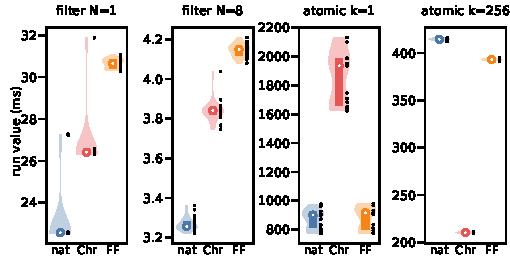
\includegraphics[width=0.9\linewidth]{../figures/campaign-distributions.pdf}
\caption{Distribution of the 30 per-run values of the filter and of the
atomic histogram, per environment.}
\Description{Violin plots of per-run medians for the filter and the atomic histogram in the three environments.}
\label{fig:distributions}
\end{figure}

\section{RQ1: Scaling Without Synchronization}
\label{sec:rq1}

The main campaign ran 3 environments $\times$ (9 workload configurations
$\times$ $N \in \{1,2,4,6,7,8\}$ + 5 sequential references) $\times$ 30
runs = 5310 runs in one random order (seed 2026112201), in 14.0 hours.
Tables~\ref{tab:times}, \ref{tab:speedup} and~\ref{tab:efficiency} give the
time, the speedup and the efficiency of every cell;
Figures~\ref{fig:speedup} and~\ref{fig:efficiency} draw them.

\begin{figure}[tbp]
\centering
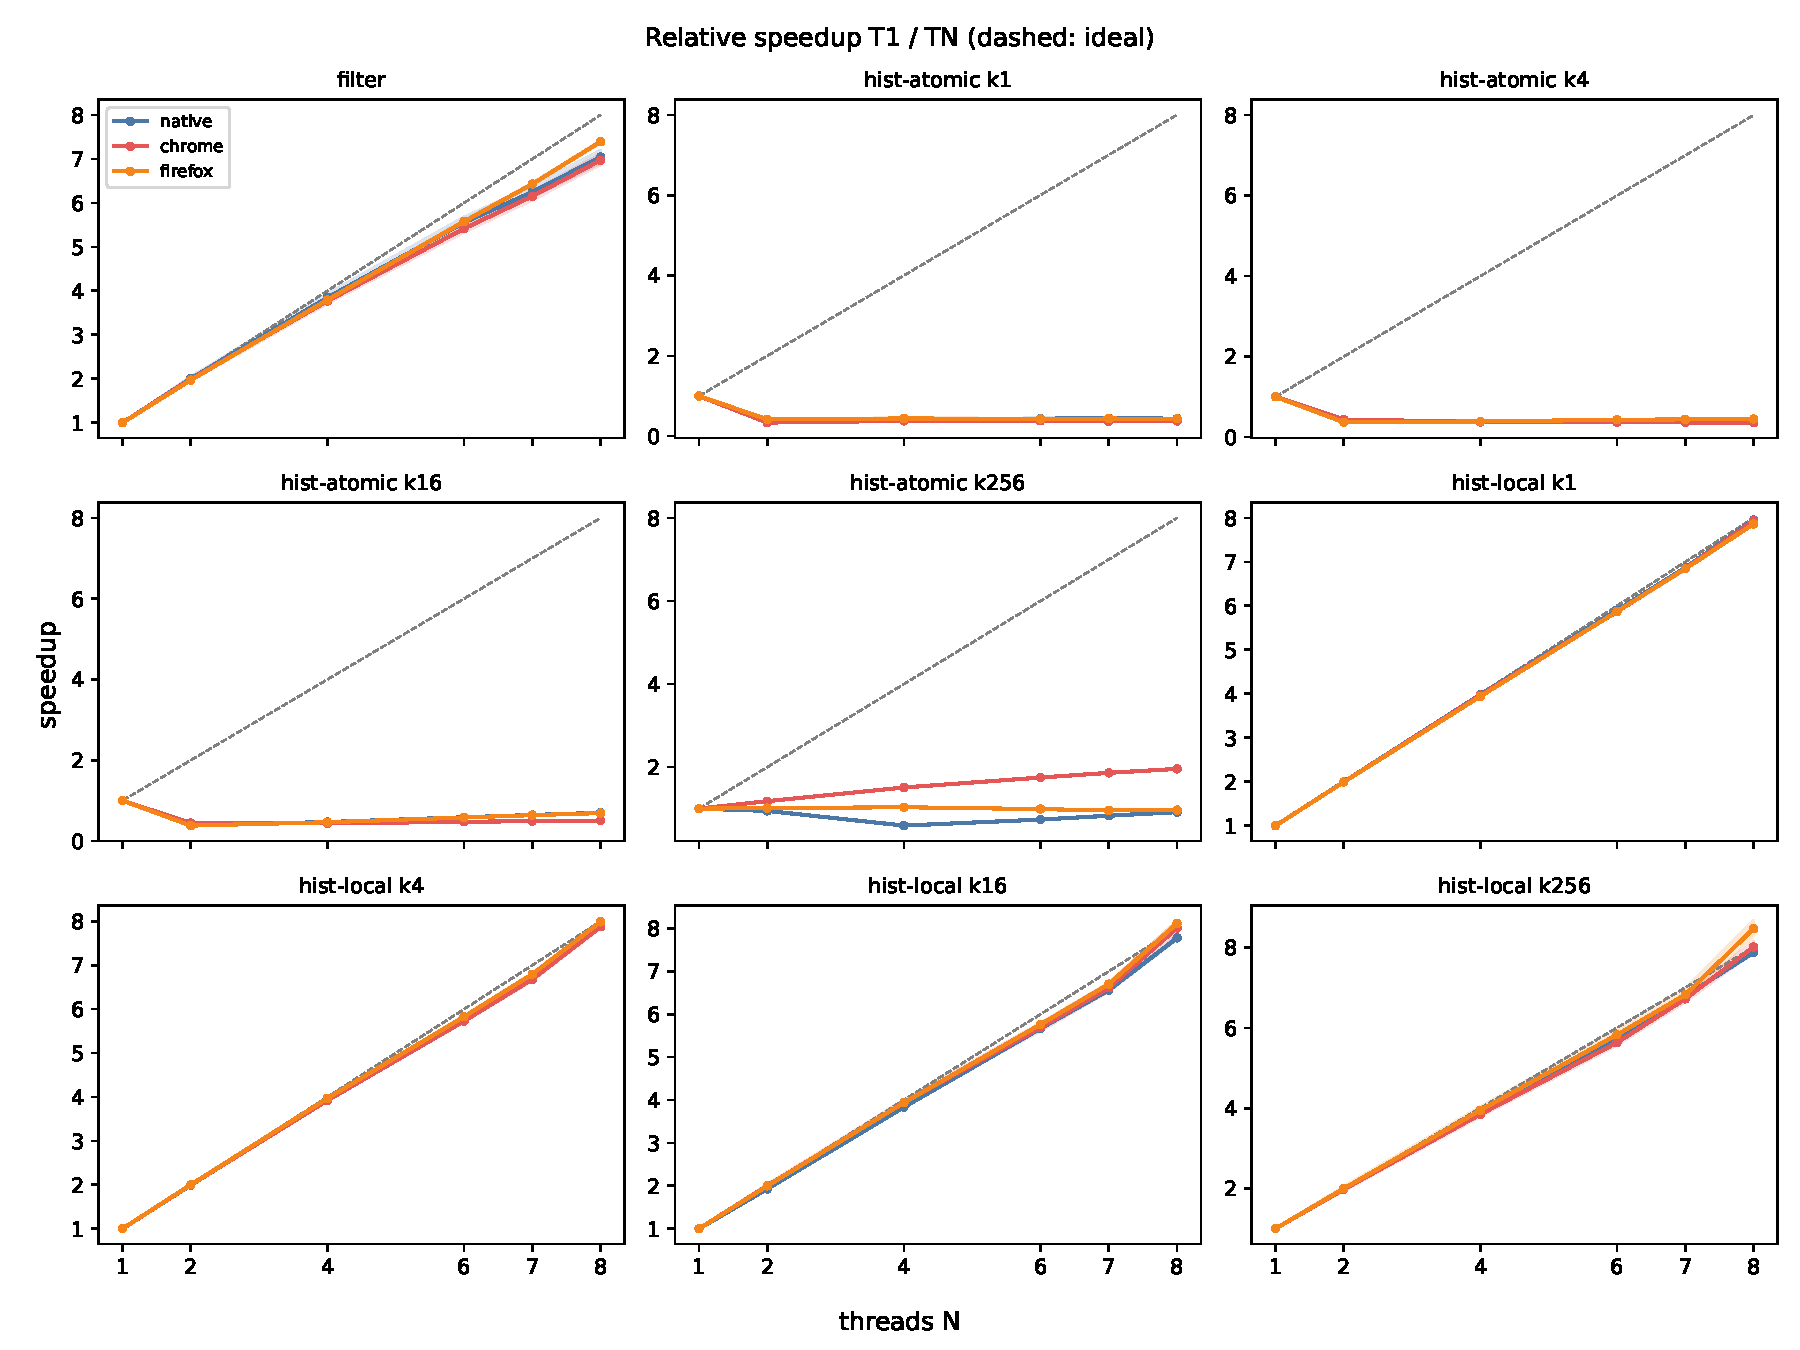
\includegraphics[width=\linewidth]{../figures/campaign-speedup.pdf}
\caption{Relative speedup against $N$ per workload (30 runs per point,
bands: 95\% CI; dashed: ideal).}
\Description{Speedup against thread count, one panel per workload, for native, Chrome and Firefox.}
\label{fig:speedup}
\end{figure}

\begin{figure}[tbp]
\centering
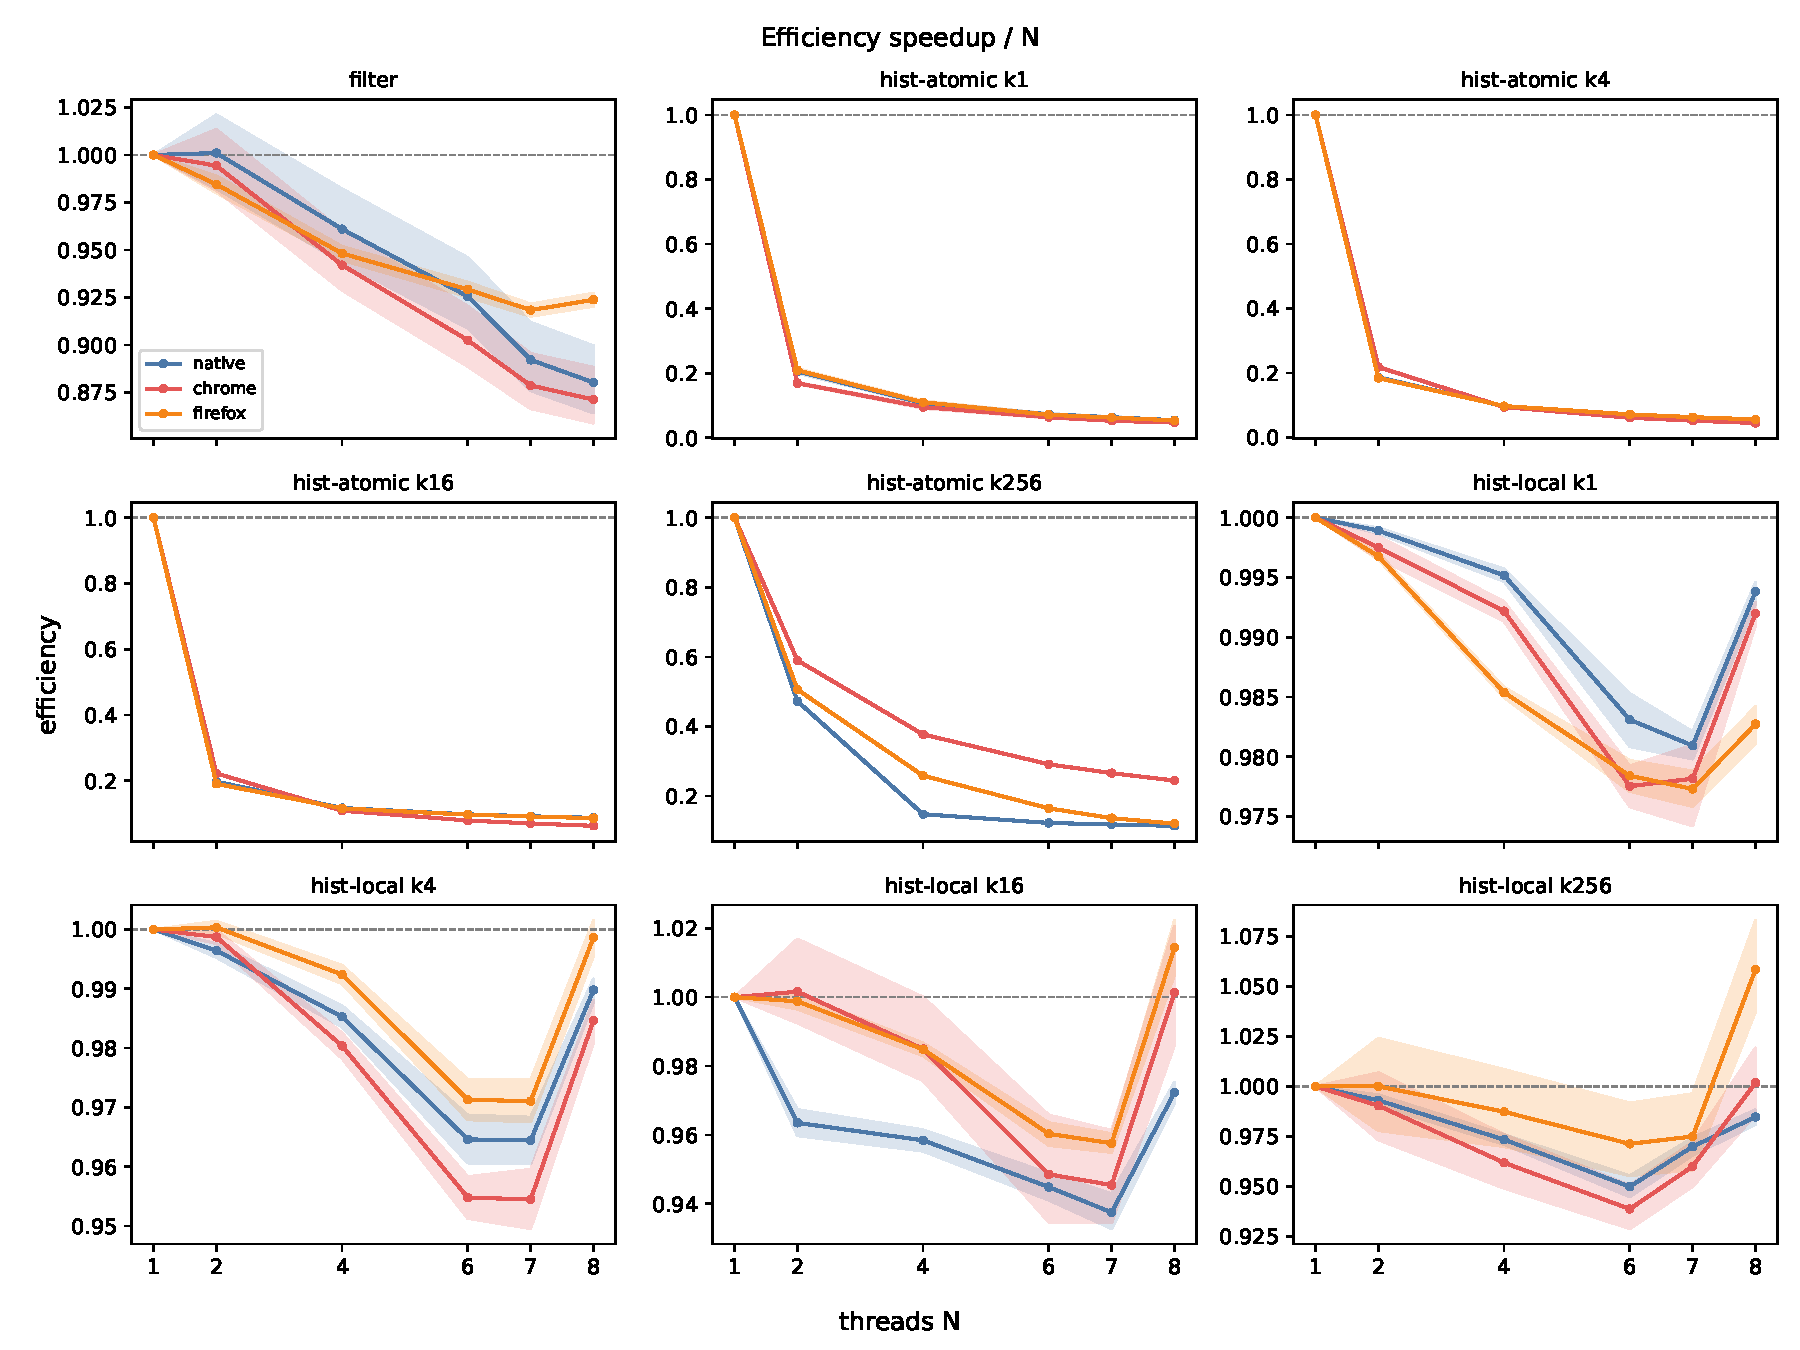
\includegraphics[width=\linewidth]{../figures/campaign-efficiency.pdf}
\caption{Efficiency $S_N/N$ against $N$ per workload (bands: 95\% CI).}
\Description{Efficiency against thread count, one panel per workload, for native, Chrome and Firefox.}
\label{fig:efficiency}
\end{figure}

\subsection{The primary result}

The filter reaches a speedup of 6.96 at $N=8$ natively (95\% CI [6.94,
6.97]), 6.92 in Chrome [6.89, 6.96] and 7.34 in Firefox [7.24, 7.42]: an
efficiency of 0.869, 0.865 and 0.917. The two primary RQ1 contrasts
(Table~\ref{tab:primary}) are the ratios of those speedups to native's:
\begin{itemize}[leftmargin=1.5em]
\item \emph{Chrome}: 0.996, 99.5\% CI [0.987, 1.004], not rejected
(Holm-adjusted $p = 0.28$). Chrome's filter speedup is within $-1.3$\% to
$+0.4$\% of native's. A non-rejection is not proof of equality; the
interval is the bound.
\item \emph{Firefox}: 1.055, 99.5\% CI [1.034, 1.072], rejected. Firefox's
speedup is 5.5\% higher than native's, from a slower baseline: its filter
takes 30.8~ms on one thread against 22.6~ms natively, and 4.20 against
3.25~ms on eight. Section~\ref{sec:why-rq1} explains why a slower loop
scales better here.
\end{itemize}

\begin{table}[htbp]
\caption{The ten primary contrasts at $N=8$: effect, 95\,\% interval, Bonferroni 99.5\,\% interval, bootstrap $p$, Holm-adjusted $p$ and the decision at $\alpha=0.05$.}\label{tab:primary}
\centering\footnotesize
\begin{tabular}{lllccrrl}
\toprule
RQ & Browser & Cell & Effect [95\,\%] & [99.5\,\%] & $p$ & Holm $p$ & Rejected \\
\midrule
RQ1 & Chrome & filter & 0.9955 [0.9896, 1.002] & [0.9868, 1.004] & 0.1416 & 0.2832 & no \\
RQ1 & Firefox & filter & 1.055 [1.041, 1.067] & [1.034, 1.072] & 0.0001 & 0.001 & yes \\
RQ2 & Chrome & atomic, $k$=1 & 2.259 [2.157, 2.365] & [2.11, 2.406] & 0.0001 & 0.001 & yes \\
RQ2 & Chrome & atomic, $k$=4 & 1.771 [1.754, 1.787] & [1.746, 1.793] & 0.0001 & 0.001 & yes \\
RQ2 & Chrome & atomic, $k$=16 & 1.425 [1.408, 1.442] & [1.399, 1.451] & 0.0001 & 0.001 & yes \\
RQ2 & Chrome & atomic, $k$=256 & 0.4159 [0.4096, 0.4222] & [0.4072, 0.4251] & 0.0001 & 0.001 & yes \\
RQ2 & Firefox & atomic, $k$=1 & 1.01 [0.9724, 1.049] & [0.9573, 1.067] & 0.5994 & 0.5994 & no \\
RQ2 & Firefox & atomic, $k$=4 & 0.9691 [0.9597, 0.9788] & [0.9555, 0.9827] & 0.0001 & 0.001 & yes \\
RQ2 & Firefox & atomic, $k$=16 & 0.8311 [0.824, 0.8385] & [0.8208, 0.8417] & 0.0001 & 0.001 & yes \\
RQ2 & Firefox & atomic, $k$=256 & 0.7965 [0.7864, 0.8058] & [0.782, 0.8089] & 0.0001 & 0.001 & yes \\
\bottomrule
\end{tabular}
\end{table}


The local histogram, which also has no shared write, reaches 7.83 to 8.48
at $N=8$ in every environment and at every $k$ (efficiency 0.98 to 1.06).
The exploratory speedup ratios of every cell are in
Table~\ref{tab:rq1-ratios}: for the local histogram they stay between 0.99
and 1.07 at $N=8$. Two features of these curves are taken up later: the
efficiency above 1 in Firefox at $k \geq 16$ (speedups of 8.26 and 8.48,
Section~\ref{sec:why-superlinear}), and a dip of the efficiency at six and
seven threads that recovers at eight, in every environment
(Section~\ref{sec:dip}).

\subsection{Absolute time: a constant factor}

A speedup compares an environment with itself.
Table~\ref{tab:absolute} and Figure~\ref{fig:absolute} give the time in the
browser over the native time at the same $N$. On one thread WASM is slower
for the filter (Chrome 1.172 times native [1.167, 1.177], Firefox 1.363
[1.356, 1.372]) and for the local histogram at $k \geq 16$ (1.23 to 1.27
times), and within 7\% at $k \leq 4$. The ratio does not grow with $N$:
for the filter at eight threads it is 1.177 in Chrome and 1.292 in Firefox.
WASM threads cost a constant factor in time, not scalability.

One cell goes the other way: at $k=1$ Chrome's local histogram is 2.7\%
\emph{faster} than native (0.973 [0.972, 0.974]). With every pixel on one
counter the loop is a chain through memory, bound by store-to-load
forwarding and not by throughput; LLVM uses one read-modify-write
instruction per pixel (\code{inc} on memory) and V8 a load, an add and a
store. An investigation on the first build timed both sequences by hand in
a native microbenchmark and reproduced the campaign's difference within
about 1\%. It is evidence from an earlier build, and it matches the
listings of v3 (Section~\ref{sec:engine-code}); the point for the reader is
that the engine's code generator is part of what is measured, in both
directions.

\begin{figure}[tbp]
\centering
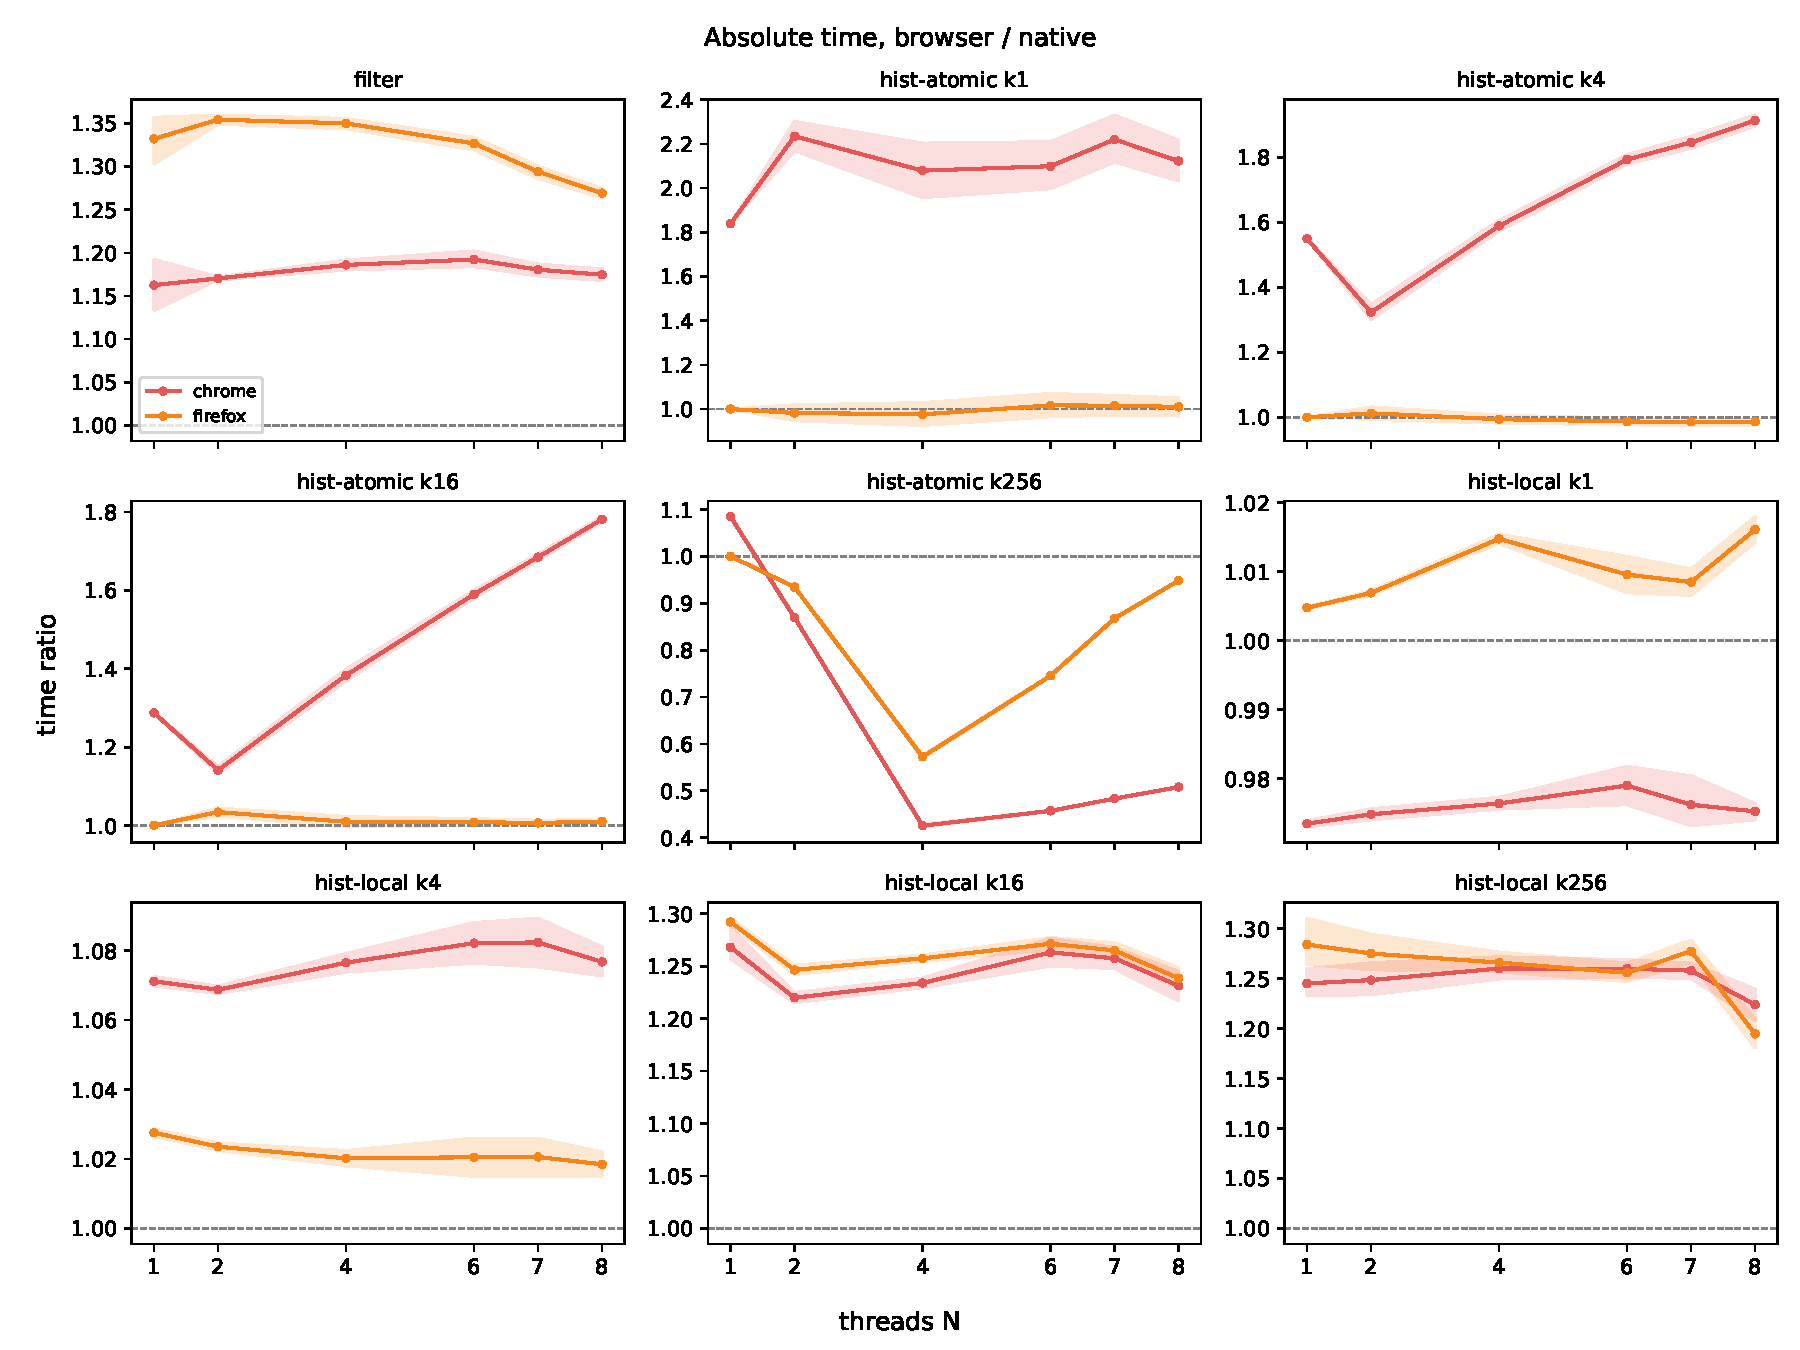
\includegraphics[width=\linewidth]{../figures/campaign-absolute.pdf}
\caption{Absolute time of one iteration against $N$ per workload and
environment.}
\Description{Absolute time against thread count per workload for the three environments.}
\label{fig:absolute}
\end{figure}

\subsection{Is the speedup inflated by a slow baseline?}
\label{sec:sequential}

Relative speedup divides by the time of a pool of one thread. If that pool
were slow compared with code that has no pool at all, every speedup would
be inflated. The sequential references answer it
(Table~\ref{tab:sequential}): the sequential kernel takes between 0.957 and
1.072 times the time of the pool of one thread, that is, the pool costs
between 7\% less and 5\% more than sequential code, in every environment.
For the filter the pool costs under 1\% natively and in Chrome and 2.5\%
in Firefox. Against the sequential reference the filter still reaches 6.90,
6.86 and 7.15 at eight threads, and the local histogram's speedup above 8
in Firefox is still there (8.09 and 8.12 at $k=16$ and 256). Natively the
sequential histogram and one task of the local histogram are the same
machine-code loop.

\begin{table}[htbp]
\caption{Sequential references: time of the kernel without Rayon in ms, the pool of one thread against it ($T_{seq}/T_1$ with its 95\,\% interval; 1 means the pool costs nothing), and the speedup of eight threads against it.}\label{tab:sequential}
\centering\scriptsize
\begin{tabular}{lrcrrcrrcr}
\toprule
 & \multicolumn{3}{c}{Native} & \multicolumn{3}{c}{Chrome} & \multicolumn{3}{c}{Firefox} \\
Workload & $T_{seq}$ & $T_{seq}/T_1$ & $T_{seq}/T_8$ & $T_{seq}$ & $T_{seq}/T_1$ & $T_{seq}/T_8$ & $T_{seq}$ & $T_{seq}/T_1$ & $T_{seq}/T_8$ \\
\midrule
filter & 22.413 & 0.9917 [0.9911, 0.9922] & 6.898 & 26.237 & 0.9906 [0.9854, 0.9958] & 6.859 & 30.035 & 0.9749 [0.9627, 0.986] & 7.152 \\
local, $k$=1 & 155.1 & 1.001 [1.001, 1.001] & 7.967 & 153.8 & 1.02 [1.019, 1.021] & 8.092 & 152.8 & 0.9815 [0.9724, 0.9885] & 7.725 \\
local, $k$=4 & 42.704 & 0.9945 [0.9939, 0.9951] & 7.907 & 43.916 & 0.9563 [0.9531, 0.9582] & 7.544 & 42.655 & 0.9703 [0.9648, 0.9747] & 7.78 \\
local, $k$=16 & 27.695 & 0.9674 [0.9596, 0.9743] & 7.607 & 38.178 & 1.072 [1.062, 1.08] & 8.395 & 35.676 & 0.979 [0.9768, 0.9813] & 8.086 \\
local, $k$=256 & 26.593 & 0.9816 [0.9741, 0.987] & 7.785 & 33.964 & 1.018 [1.003, 1.03] & 8.149 & 32.993 & 0.9566 [0.9363, 0.9728] & 8.116 \\
\bottomrule
\end{tabular}
\end{table}


Table~\ref{tab:throughput} gives the same data as nanoseconds per pixel and
as the \emph{absolute} speedup, the native one-thread time over the time of
the environment at $N$: on eight threads the filter is 6.96 times faster
than one native thread natively, 5.91 times in Chrome and 5.38 times in
Firefox.

\subsection{Fork-join: what does not divide with the work}
\label{sec:forkjoin}

The constant factor divides with the work; the cost of starting and ending
a parallel region does not. The calibration of every run measures it
(Table~\ref{tab:fork-join}). With the workers awake (warm), an empty
\code{broadcast} at $N=8$ takes 110~\textmu s in Chrome and 60~\textmu s in
Firefox against 7.9~\textmu s natively (medians over 270 runs of the
per-run median), and an empty parallel iterator 25, 20 and 5.4~\textmu s.
The means are larger (164, 91 and 46~\textmu s for the broadcast), so the
distribution has a tail. Three cautions go with these numbers:
\begin{itemize}[leftmargin=1.5em]
\item \emph{Resolution.} With a 20~\textmu s clock, Firefox's warm values
are multiples of 20 and read 0 at $N \leq 4$; Chrome's are multiples of 5.
Twenty samples per probe do not resolve them better.
\item \emph{A step at $N=8$.} Natively the broadcast takes 1.8 to
3.1~\textmu s up to $N=7$ and 7.9 at $N=8$, and Chrome's goes from 10 to
110. At eight threads the coordinating thread shares the eight cores with
eight workers; that this is the cause was not tested.
\item \emph{Cold depends on what ran before.} After a pause the workers are
asleep, as before a measured iteration. In filter runs the cold broadcast
at $N=8$ takes 205~\textmu s natively, 460 in Chrome and 270 in Firefox; in
histogram runs 31 to 34, 65 and 80 to 85, so that Chrome's cold call is
cheaper than its warm one there. The pause is as long as the workload's
checksum, which differs between workloads; the cause is not established.
\end{itemize}
With iterations of milliseconds these costs are amortized (0.33\% of $T_8$
natively at 8192$^2$, 1.4\% in Firefox and 2.7\% in Chrome with the warm
cost, Section~\ref{sec:cutoff}); with regions under a millisecond they are a
large share of the time.

\subsection{Karp-Flatt}

Table~\ref{tab:karp-flatt} gives the serial fraction that Amdahl's law
would need to explain each speedup. For the filter at $N=8$ it is 0.021
natively, 0.022 in Chrome and 0.013 in Firefox, and it does not fall as $N$
grows (natively 0.018, 0.019, 0.021 at $N=2$, 4, 8). But the timed region
of the filter has no serial part: every row is processed in parallel and
nothing else is timed. So $e$ here is not serial code, it is a cost of
running in parallel, and Section~\ref{sec:why-rq1} attributes about half of
it natively to the cores' own slower work on shared memory. For the local
histogram $e$ is between $-0.008$ and $0.013$ from $N=4$ on.

{\small
\begin{longtable}{llrrr}
\caption{Main campaign: time of one iteration in ms (geometric mean over 30 runs of the per-run median of 10 measured iterations).}\label{tab:times} \\
\toprule
Workload & $N$ & Native & Chrome & Firefox \\
\midrule
\endfirsthead
\toprule
Workload & $N$ & Native & Chrome & Firefox \\
\midrule
\endhead
\bottomrule
\endfoot
filter & 1 & 22.601 & 26.486 & 30.808 \\
filter & 2 & 11.502 & 13.505 & 15.641 \\
filter & 4 & 5.979 & 7.111 & 8.146 \\
filter & 6 & 4.140 & 4.909 & 5.535 \\
filter & 7 & 3.658 & 4.350 & 4.814 \\
filter & 8 & 3.249 & 3.825 & 4.200 \\
\midrule
atomic, $k$=1 & 1 & 379.6 & 698.0 & 379.7 \\
atomic, $k$=1 & 2 & 901.0 & 2028.1 & 932.4 \\
atomic, $k$=1 & 4 & 842.0 & 1905.8 & 849.2 \\
atomic, $k$=1 & 6 & 838.0 & 1868.5 & 869.0 \\
atomic, $k$=1 & 7 & 885.4 & 1876.6 & 900.3 \\
atomic, $k$=1 & 8 & 856.3 & 1888.8 & 878.5 \\
\midrule
atomic, $k$=4 & 1 & 379.6 & 588.7 & 379.7 \\
atomic, $k$=4 & 2 & 1009.8 & 1362.6 & 1025.0 \\
atomic, $k$=4 & 4 & 976.8 & 1546.2 & 970.8 \\
atomic, $k$=4 & 6 & 900.9 & 1613.4 & 885.0 \\
atomic, $k$=4 & 7 & 870.8 & 1631.9 & 866.4 \\
atomic, $k$=4 & 8 & 863.6 & 1648.4 & 849.6 \\
\midrule
atomic, $k$=16 & 1 & 379.5 & 488.5 & 379.8 \\
atomic, $k$=16 & 2 & 957.3 & 1099.9 & 989.7 \\
atomic, $k$=16 & 4 & 805.7 & 1124.1 & 819.7 \\
atomic, $k$=16 & 6 & 646.1 & 1029.5 & 651.1 \\
atomic, $k$=16 & 7 & 588.6 & 992.7 & 593.2 \\
atomic, $k$=16 & 8 & 544.0 & 968.4 & 548.0 \\
\midrule
atomic, $k$=256 & 1 & 379.6 & 411.9 & 379.8 \\
atomic, $k$=256 & 2 & 401.5 & 349.0 & 375.2 \\
atomic, $k$=256 & 4 & 639.7 & 273.9 & 368.2 \\
atomic, $k$=256 & 6 & 515.8 & 235.2 & 383.9 \\
atomic, $k$=256 & 7 & 458.1 & 221.3 & 396.7 \\
atomic, $k$=256 & 8 & 414.6 & 210.4 & 393.0 \\
\midrule
local, $k$=1 & 1 & 154.9 & 150.7 & 155.6 \\
local, $k$=1 & 2 & 77.581 & 75.511 & 78.060 \\
local, $k$=1 & 4 & 38.929 & 37.992 & 39.485 \\
local, $k$=1 & 6 & 26.250 & 25.759 & 26.515 \\
local, $k$=1 & 7 & 22.562 & 21.981 & 22.752 \\
local, $k$=1 & 8 & 19.473 & 19.011 & 19.775 \\
\midrule
local, $k$=4 & 1 & 42.939 & 45.924 & 43.961 \\
local, $k$=4 & 2 & 21.481 & 22.940 & 21.958 \\
local, $k$=4 & 4 & 10.868 & 11.679 & 11.044 \\
local, $k$=4 & 6 & 7.382 & 8.005 & 7.554 \\
local, $k$=4 & 7 & 6.339 & 6.897 & 6.451 \\
local, $k$=4 & 8 & 5.401 & 5.822 & 5.482 \\
\midrule
local, $k$=16 & 1 & 28.627 & 35.616 & 36.440 \\
local, $k$=16 & 2 & 14.764 & 17.882 & 18.071 \\
local, $k$=16 & 4 & 7.395 & 9.051 & 9.188 \\
local, $k$=16 & 6 & 4.988 & 6.276 & 6.292 \\
local, $k$=16 & 7 & 4.297 & 5.390 & 5.412 \\
local, $k$=16 & 8 & 3.640 & 4.548 & 4.412 \\
\midrule
local, $k$=256 & 1 & 27.092 & 33.367 & 34.491 \\
local, $k$=256 & 2 & 13.597 & 16.742 & 17.268 \\
local, $k$=256 & 4 & 6.934 & 8.626 & 8.866 \\
local, $k$=256 & 6 & 4.752 & 5.930 & 5.976 \\
local, $k$=256 & 7 & 3.984 & 4.997 & 5.066 \\
local, $k$=256 & 8 & 3.416 & 4.168 & 4.065 \\
\end{longtable}
}

{\small
\begin{longtable}{llccc}
\caption{Main campaign: relative speedup $T_1/T_N$ with its 95\,\% bootstrap interval (30 runs per cell, geometric mean of the per-run medians).}\label{tab:speedup} \\
\toprule
Workload & $N$ & Native & Chrome & Firefox \\
\midrule
\endfirsthead
\toprule
Workload & $N$ & Native & Chrome & Firefox \\
\midrule
\endhead
\bottomrule
\endfoot
filter & 1 & 1.000 [1.000, 1.000] & 1.000 [1.000, 1.000] & 1.000 [1.000, 1.000] \\
filter & 2 & 1.965 [1.963, 1.967] & 1.961 [1.944, 1.977] & 1.970 [1.947, 1.991] \\
filter & 4 & 3.780 [3.774, 3.786] & 3.725 [3.702, 3.747] & 3.782 [3.727, 3.830] \\
filter & 6 & 5.459 [5.440, 5.475] & 5.396 [5.367, 5.424] & 5.566 [5.511, 5.619] \\
filter & 7 & 6.179 [6.166, 6.190] & 6.088 [6.055, 6.121] & 6.400 [6.341, 6.457] \\
filter & 8 & 6.955 [6.942, 6.969] & 6.924 [6.885, 6.964] & 7.336 [7.235, 7.422] \\
\midrule
atomic, $k$=1 & 1 & 1.000 [1.000, 1.000] & 1.000 [1.000, 1.000] & 1.000 [1.000, 1.000] \\
atomic, $k$=1 & 2 & 0.421 [0.412, 0.430] & 0.344 [0.338, 0.351] & 0.407 [0.394, 0.420] \\
atomic, $k$=1 & 4 & 0.451 [0.434, 0.468] & 0.366 [0.351, 0.382] & 0.447 [0.434, 0.461] \\
atomic, $k$=1 & 6 & 0.453 [0.437, 0.469] & 0.374 [0.360, 0.388] & 0.437 [0.423, 0.452] \\
atomic, $k$=1 & 7 & 0.429 [0.416, 0.444] & 0.372 [0.359, 0.386] & 0.422 [0.411, 0.435] \\
atomic, $k$=1 & 8 & 0.443 [0.431, 0.455] & 0.370 [0.357, 0.384] & 0.432 [0.421, 0.444] \\
\midrule
atomic, $k$=4 & 1 & 1.000 [1.000, 1.000] & 1.000 [1.000, 1.000] & 1.000 [1.000, 1.000] \\
atomic, $k$=4 & 2 & 0.376 [0.371, 0.381] & 0.432 [0.428, 0.436] & 0.370 [0.367, 0.374] \\
atomic, $k$=4 & 4 & 0.389 [0.386, 0.392] & 0.381 [0.378, 0.384] & 0.391 [0.388, 0.395] \\
atomic, $k$=4 & 6 & 0.421 [0.418, 0.425] & 0.365 [0.363, 0.367] & 0.429 [0.426, 0.432] \\
atomic, $k$=4 & 7 & 0.436 [0.433, 0.439] & 0.361 [0.359, 0.363] & 0.438 [0.435, 0.441] \\
atomic, $k$=4 & 8 & 0.440 [0.436, 0.443] & 0.357 [0.355, 0.359] & 0.447 [0.445, 0.449] \\
\midrule
atomic, $k$=16 & 1 & 1.000 [1.000, 1.000] & 1.000 [1.000, 1.000] & 1.000 [1.000, 1.000] \\
atomic, $k$=16 & 2 & 0.396 [0.393, 0.400] & 0.444 [0.441, 0.447] & 0.384 [0.381, 0.386] \\
atomic, $k$=16 & 4 & 0.471 [0.466, 0.476] & 0.435 [0.433, 0.437] & 0.463 [0.459, 0.468] \\
atomic, $k$=16 & 6 & 0.587 [0.585, 0.590] & 0.474 [0.473, 0.476] & 0.583 [0.580, 0.586] \\
atomic, $k$=16 & 7 & 0.645 [0.642, 0.647] & 0.492 [0.491, 0.494] & 0.640 [0.637, 0.643] \\
atomic, $k$=16 & 8 & 0.698 [0.695, 0.700] & 0.504 [0.503, 0.506] & 0.693 [0.691, 0.696] \\
\midrule
atomic, $k$=256 & 1 & 1.000 [1.000, 1.000] & 1.000 [1.000, 1.000] & 1.000 [1.000, 1.000] \\
atomic, $k$=256 & 2 & 0.945 [0.945, 0.946] & 1.180 [1.179, 1.180] & 1.012 [1.012, 1.012] \\
atomic, $k$=256 & 4 & 0.593 [0.589, 0.597] & 1.504 [1.499, 1.509] & 1.031 [1.030, 1.033] \\
atomic, $k$=256 & 6 & 0.736 [0.734, 0.738] & 1.751 [1.747, 1.755] & 0.989 [0.988, 0.991] \\
atomic, $k$=256 & 7 & 0.829 [0.827, 0.831] & 1.861 [1.859, 1.863] & 0.957 [0.956, 0.959] \\
atomic, $k$=256 & 8 & 0.916 [0.915, 0.916] & 1.958 [1.957, 1.959] & 0.966 [0.966, 0.967] \\
\midrule
local, $k$=1 & 1 & 1.000 [1.000, 1.000] & 1.000 [1.000, 1.000] & 1.000 [1.000, 1.000] \\
local, $k$=1 & 2 & 1.997 [1.997, 1.997] & 1.996 [1.995, 1.998] & 1.994 [1.993, 1.994] \\
local, $k$=1 & 4 & 3.980 [3.978, 3.982] & 3.968 [3.964, 3.971] & 3.942 [3.940, 3.944] \\
local, $k$=1 & 6 & 5.902 [5.886, 5.917] & 5.852 [5.842, 5.862] & 5.870 [5.859, 5.880] \\
local, $k$=1 & 7 & 6.867 [6.859, 6.874] & 6.858 [6.845, 6.871] & 6.840 [6.830, 6.851] \\
local, $k$=1 & 8 & 7.956 [7.951, 7.959] & 7.930 [7.923, 7.936] & 7.870 [7.862, 7.878] \\
\midrule
local, $k$=4 & 1 & 1.000 [1.000, 1.000] & 1.000 [1.000, 1.000] & 1.000 [1.000, 1.000] \\
local, $k$=4 & 2 & 1.999 [1.998, 2.000] & 2.002 [2.000, 2.004] & 2.002 [2.001, 2.004] \\
local, $k$=4 & 4 & 3.951 [3.945, 3.957] & 3.932 [3.923, 3.941] & 3.980 [3.975, 3.985] \\
local, $k$=4 & 6 & 5.817 [5.797, 5.837] & 5.737 [5.719, 5.756] & 5.820 [5.797, 5.843] \\
local, $k$=4 & 7 & 6.774 [6.757, 6.791] & 6.658 [6.630, 6.687] & 6.815 [6.789, 6.841] \\
local, $k$=4 & 8 & 7.950 [7.939, 7.961] & 7.889 [7.858, 7.917] & 8.019 [7.989, 8.048] \\
\midrule
local, $k$=16 & 1 & 1.000 [1.000, 1.000] & 1.000 [1.000, 1.000] & 1.000 [1.000, 1.000] \\
local, $k$=16 & 2 & 1.939 [1.933, 1.945] & 1.992 [1.985, 1.999] & 2.017 [2.012, 2.022] \\
local, $k$=16 & 4 & 3.871 [3.860, 3.882] & 3.935 [3.920, 3.951] & 3.966 [3.956, 3.976] \\
local, $k$=16 & 6 & 5.739 [5.714, 5.765] & 5.675 [5.644, 5.706] & 5.791 [5.770, 5.814] \\
local, $k$=16 & 7 & 6.663 [6.628, 6.700] & 6.607 [6.553, 6.667] & 6.733 [6.713, 6.754] \\
local, $k$=16 & 8 & 7.864 [7.835, 7.890] & 7.832 [7.743, 7.921] & 8.259 [8.204, 8.313] \\
\midrule
local, $k$=256 & 1 & 1.000 [1.000, 1.000] & 1.000 [1.000, 1.000] & 1.000 [1.000, 1.000] \\
local, $k$=256 & 2 & 1.993 [1.988, 1.997] & 1.993 [1.970, 2.016] & 1.997 [1.959, 2.043] \\
local, $k$=256 & 4 & 3.907 [3.897, 3.917] & 3.868 [3.836, 3.909] & 3.890 [3.824, 3.974] \\
local, $k$=256 & 6 & 5.701 [5.654, 5.741] & 5.627 [5.567, 5.699] & 5.771 [5.683, 5.890] \\
local, $k$=256 & 7 & 6.800 [6.772, 6.828] & 6.677 [6.621, 6.748] & 6.808 [6.703, 6.949] \\
local, $k$=256 & 8 & 7.931 [7.912, 7.949] & 8.006 [7.874, 8.147] & 8.484 [8.325, 8.677] \\
\end{longtable}
}

{\small
\begin{longtable}{llccc}
\caption{Main campaign: efficiency $S_N/N$ with its 95\,\% bootstrap interval.}\label{tab:efficiency} \\
\toprule
Workload & $N$ & Native & Chrome & Firefox \\
\midrule
\endfirsthead
\toprule
Workload & $N$ & Native & Chrome & Firefox \\
\midrule
\endhead
\bottomrule
\endfoot
filter & 1 & 1.000 [1.000, 1.000] & 1.000 [1.000, 1.000] & 1.000 [1.000, 1.000] \\
filter & 2 & 0.982 [0.982, 0.983] & 0.981 [0.972, 0.989] & 0.985 [0.974, 0.995] \\
filter & 4 & 0.945 [0.943, 0.946] & 0.931 [0.926, 0.937] & 0.945 [0.932, 0.958] \\
filter & 6 & 0.910 [0.907, 0.913] & 0.899 [0.895, 0.904] & 0.928 [0.919, 0.937] \\
filter & 7 & 0.883 [0.881, 0.884] & 0.870 [0.865, 0.874] & 0.914 [0.906, 0.922] \\
filter & 8 & 0.869 [0.868, 0.871] & 0.865 [0.861, 0.870] & 0.917 [0.904, 0.928] \\
\midrule
atomic, $k$=1 & 1 & 1.000 [1.000, 1.000] & 1.000 [1.000, 1.000] & 1.000 [1.000, 1.000] \\
atomic, $k$=1 & 2 & 0.211 [0.206, 0.215] & 0.172 [0.169, 0.175] & 0.204 [0.197, 0.210] \\
atomic, $k$=1 & 4 & 0.113 [0.108, 0.117] & 0.092 [0.088, 0.096] & 0.112 [0.109, 0.115] \\
atomic, $k$=1 & 6 & 0.076 [0.073, 0.078] & 0.062 [0.060, 0.065] & 0.073 [0.070, 0.075] \\
atomic, $k$=1 & 7 & 0.061 [0.059, 0.063] & 0.053 [0.051, 0.055] & 0.060 [0.059, 0.062] \\
atomic, $k$=1 & 8 & 0.055 [0.054, 0.057] & 0.046 [0.045, 0.048] & 0.054 [0.053, 0.056] \\
\midrule
atomic, $k$=4 & 1 & 1.000 [1.000, 1.000] & 1.000 [1.000, 1.000] & 1.000 [1.000, 1.000] \\
atomic, $k$=4 & 2 & 0.188 [0.186, 0.190] & 0.216 [0.214, 0.218] & 0.185 [0.184, 0.187] \\
atomic, $k$=4 & 4 & 0.097 [0.096, 0.098] & 0.095 [0.094, 0.096] & 0.098 [0.097, 0.099] \\
atomic, $k$=4 & 6 & 0.070 [0.070, 0.071] & 0.061 [0.060, 0.061] & 0.072 [0.071, 0.072] \\
atomic, $k$=4 & 7 & 0.062 [0.062, 0.063] & 0.052 [0.051, 0.052] & 0.063 [0.062, 0.063] \\
atomic, $k$=4 & 8 & 0.055 [0.055, 0.055] & 0.045 [0.044, 0.045] & 0.056 [0.056, 0.056] \\
\midrule
atomic, $k$=16 & 1 & 1.000 [1.000, 1.000] & 1.000 [1.000, 1.000] & 1.000 [1.000, 1.000] \\
atomic, $k$=16 & 2 & 0.198 [0.197, 0.200] & 0.222 [0.221, 0.224] & 0.192 [0.191, 0.193] \\
atomic, $k$=16 & 4 & 0.118 [0.117, 0.119] & 0.109 [0.108, 0.109] & 0.116 [0.115, 0.117] \\
atomic, $k$=16 & 6 & 0.098 [0.097, 0.098] & 0.079 [0.079, 0.079] & 0.097 [0.097, 0.098] \\
atomic, $k$=16 & 7 & 0.092 [0.092, 0.092] & 0.070 [0.070, 0.071] & 0.091 [0.091, 0.092] \\
atomic, $k$=16 & 8 & 0.087 [0.087, 0.088] & 0.063 [0.063, 0.063] & 0.087 [0.086, 0.087] \\
\midrule
atomic, $k$=256 & 1 & 1.000 [1.000, 1.000] & 1.000 [1.000, 1.000] & 1.000 [1.000, 1.000] \\
atomic, $k$=256 & 2 & 0.473 [0.473, 0.473] & 0.590 [0.590, 0.590] & 0.506 [0.506, 0.506] \\
atomic, $k$=256 & 4 & 0.148 [0.147, 0.149] & 0.376 [0.375, 0.377] & 0.258 [0.257, 0.258] \\
atomic, $k$=256 & 6 & 0.123 [0.122, 0.123] & 0.292 [0.291, 0.292] & 0.165 [0.165, 0.165] \\
atomic, $k$=256 & 7 & 0.118 [0.118, 0.119] & 0.266 [0.266, 0.266] & 0.137 [0.137, 0.137] \\
atomic, $k$=256 & 8 & 0.114 [0.114, 0.115] & 0.245 [0.245, 0.245] & 0.121 [0.121, 0.121] \\
\midrule
local, $k$=1 & 1 & 1.000 [1.000, 1.000] & 1.000 [1.000, 1.000] & 1.000 [1.000, 1.000] \\
local, $k$=1 & 2 & 0.998 [0.998, 0.999] & 0.998 [0.997, 0.999] & 0.997 [0.997, 0.997] \\
local, $k$=1 & 4 & 0.995 [0.994, 0.995] & 0.992 [0.991, 0.993] & 0.985 [0.985, 0.986] \\
local, $k$=1 & 6 & 0.984 [0.981, 0.986] & 0.975 [0.974, 0.977] & 0.978 [0.976, 0.980] \\
local, $k$=1 & 7 & 0.981 [0.980, 0.982] & 0.980 [0.978, 0.982] & 0.977 [0.976, 0.979] \\
local, $k$=1 & 8 & 0.994 [0.994, 0.995] & 0.991 [0.990, 0.992] & 0.984 [0.983, 0.985] \\
\midrule
local, $k$=4 & 1 & 1.000 [1.000, 1.000] & 1.000 [1.000, 1.000] & 1.000 [1.000, 1.000] \\
local, $k$=4 & 2 & 0.999 [0.999, 1.000] & 1.001 [1.000, 1.002] & 1.001 [1.000, 1.002] \\
local, $k$=4 & 4 & 0.988 [0.986, 0.989] & 0.983 [0.981, 0.985] & 0.995 [0.994, 0.996] \\
local, $k$=4 & 6 & 0.970 [0.966, 0.973] & 0.956 [0.953, 0.959] & 0.970 [0.966, 0.974] \\
local, $k$=4 & 7 & 0.968 [0.965, 0.970] & 0.951 [0.947, 0.955] & 0.974 [0.970, 0.977] \\
local, $k$=4 & 8 & 0.994 [0.992, 0.995] & 0.986 [0.982, 0.990] & 1.002 [0.999, 1.006] \\
\midrule
local, $k$=16 & 1 & 1.000 [1.000, 1.000] & 1.000 [1.000, 1.000] & 1.000 [1.000, 1.000] \\
local, $k$=16 & 2 & 0.969 [0.967, 0.972] & 0.996 [0.992, 0.999] & 1.008 [1.006, 1.011] \\
local, $k$=16 & 4 & 0.968 [0.965, 0.970] & 0.984 [0.980, 0.988] & 0.992 [0.989, 0.994] \\
local, $k$=16 & 6 & 0.956 [0.952, 0.961] & 0.946 [0.941, 0.951] & 0.965 [0.962, 0.969] \\
local, $k$=16 & 7 & 0.952 [0.947, 0.957] & 0.944 [0.936, 0.952] & 0.962 [0.959, 0.965] \\
local, $k$=16 & 8 & 0.983 [0.979, 0.986] & 0.979 [0.968, 0.990] & 1.032 [1.026, 1.039] \\
\midrule
local, $k$=256 & 1 & 1.000 [1.000, 1.000] & 1.000 [1.000, 1.000] & 1.000 [1.000, 1.000] \\
local, $k$=256 & 2 & 0.996 [0.994, 0.999] & 0.996 [0.985, 1.008] & 0.999 [0.980, 1.021] \\
local, $k$=256 & 4 & 0.977 [0.974, 0.979] & 0.967 [0.959, 0.977] & 0.973 [0.956, 0.994] \\
local, $k$=256 & 6 & 0.950 [0.942, 0.957] & 0.938 [0.928, 0.950] & 0.962 [0.947, 0.982] \\
local, $k$=256 & 7 & 0.971 [0.967, 0.975] & 0.954 [0.946, 0.964] & 0.973 [0.958, 0.993] \\
local, $k$=256 & 8 & 0.991 [0.989, 0.994] & 1.001 [0.984, 1.018] & 1.061 [1.041, 1.085] \\
\end{longtable}
}

{\small
\begin{longtable}{llcc}
\caption{Main campaign: time in the browser over the native time at the same $N$, with its 95\,\% bootstrap interval (exploratory).}\label{tab:absolute} \\
\toprule
Workload & $N$ & Chrome & Firefox \\
\midrule
\endfirsthead
\toprule
Workload & $N$ & Chrome & Firefox \\
\midrule
\endhead
\bottomrule
\endfoot
filter & 1 & 1.172 [1.167, 1.177] & 1.363 [1.356, 1.372] \\
filter & 2 & 1.174 [1.166, 1.184] & 1.36 [1.348, 1.373] \\
filter & 4 & 1.189 [1.184, 1.195] & 1.362 [1.347, 1.381] \\
filter & 6 & 1.186 [1.18, 1.191] & 1.337 [1.326, 1.348] \\
filter & 7 & 1.189 [1.184, 1.194] & 1.316 [1.307, 1.326] \\
filter & 8 & 1.177 [1.172, 1.183] & 1.292 [1.28, 1.309] \\
\midrule
atomic, $k$=1 & 1 & 1.839 [1.839, 1.839] & 1 [1, 1] \\
atomic, $k$=1 & 2 & 2.251 [2.187, 2.316] & 1.035 [0.9963, 1.076] \\
atomic, $k$=1 & 4 & 2.264 [2.137, 2.396] & 1.009 [0.9607, 1.058] \\
atomic, $k$=1 & 6 & 2.23 [2.119, 2.345] & 1.037 [0.988, 1.086] \\
atomic, $k$=1 & 7 & 2.12 [2.022, 2.225] & 1.017 [0.9744, 1.062] \\
atomic, $k$=1 & 8 & 2.206 [2.107, 2.308] & 1.026 [0.9866, 1.065] \\
\midrule
atomic, $k$=4 & 1 & 1.551 [1.549, 1.554] & 1 [1, 1] \\
atomic, $k$=4 & 2 & 1.349 [1.329, 1.37] & 1.015 [1, 1.031] \\
atomic, $k$=4 & 4 & 1.583 [1.567, 1.6] & 0.9939 [0.9821, 1.006] \\
atomic, $k$=4 & 6 & 1.791 [1.775, 1.808] & 0.9823 [0.9727, 0.9925] \\
atomic, $k$=4 & 7 & 1.874 [1.858, 1.89] & 0.9949 [0.9855, 1.004] \\
atomic, $k$=4 & 8 & 1.909 [1.892, 1.925] & 0.9837 [0.9751, 0.9928] \\
\midrule
atomic, $k$=16 & 1 & 1.287 [1.286, 1.288] & 1.001 [1.001, 1.001] \\
atomic, $k$=16 & 2 & 1.149 [1.137, 1.161] & 1.034 [1.023, 1.045] \\
atomic, $k$=16 & 4 & 1.395 [1.379, 1.412] & 1.017 [1.003, 1.032] \\
atomic, $k$=16 & 6 & 1.593 [1.585, 1.602] & 1.008 [1.001, 1.015] \\
atomic, $k$=16 & 7 & 1.687 [1.678, 1.695] & 1.008 [1.002, 1.014] \\
atomic, $k$=16 & 8 & 1.78 [1.772, 1.789] & 1.007 [1.002, 1.013] \\
\midrule
atomic, $k$=256 & 1 & 1.085 [1.085, 1.085] & 1.001 [1.001, 1.001] \\
atomic, $k$=256 & 2 & 0.8694 [0.869, 0.8699] & 0.9345 [0.9343, 0.9348] \\
atomic, $k$=256 & 4 & 0.4282 [0.4251, 0.4314] & 0.5756 [0.5718, 0.5796] \\
atomic, $k$=256 & 6 & 0.456 [0.4546, 0.4575] & 0.7443 [0.7423, 0.7464] \\
atomic, $k$=256 & 7 & 0.4831 [0.4818, 0.4845] & 0.866 [0.8635, 0.8686] \\
atomic, $k$=256 & 8 & 0.5074 [0.5068, 0.508] & 0.9479 [0.9468, 0.949] \\
\midrule
local, $k$=1 & 1 & 0.973 [0.9724, 0.9736] & 1.005 [1.004, 1.005] \\
local, $k$=1 & 2 & 0.9733 [0.9727, 0.9739] & 1.006 [1.006, 1.006] \\
local, $k$=1 & 4 & 0.9759 [0.9753, 0.9766] & 1.014 [1.014, 1.015] \\
local, $k$=1 & 6 & 0.9813 [0.9783, 0.9842] & 1.01 [1.007, 1.013] \\
local, $k$=1 & 7 & 0.9743 [0.9723, 0.9763] & 1.008 [1.007, 1.01] \\
local, $k$=1 & 8 & 0.9762 [0.9755, 0.977] & 1.015 [1.014, 1.017] \\
\midrule
local, $k$=4 & 1 & 1.07 [1.069, 1.071] & 1.024 [1.023, 1.025] \\
local, $k$=4 & 2 & 1.068 [1.067, 1.069] & 1.022 [1.021, 1.023] \\
local, $k$=4 & 4 & 1.075 [1.072, 1.078] & 1.016 [1.014, 1.018] \\
local, $k$=4 & 6 & 1.084 [1.079, 1.089] & 1.023 [1.018, 1.029] \\
local, $k$=4 & 7 & 1.088 [1.083, 1.093] & 1.018 [1.013, 1.022] \\
local, $k$=4 & 8 & 1.078 [1.074, 1.082] & 1.015 [1.011, 1.019] \\
\midrule
local, $k$=16 & 1 & 1.244 [1.24, 1.248] & 1.273 [1.27, 1.276] \\
local, $k$=16 & 2 & 1.211 [1.207, 1.215] & 1.224 [1.221, 1.228] \\
local, $k$=16 & 4 & 1.224 [1.22, 1.228] & 1.242 [1.239, 1.246] \\
local, $k$=16 & 6 & 1.258 [1.25, 1.266] & 1.261 [1.255, 1.268] \\
local, $k$=16 & 7 & 1.255 [1.242, 1.266] & 1.26 [1.253, 1.267] \\
local, $k$=16 & 8 & 1.249 [1.235, 1.264] & 1.212 [1.203, 1.221] \\
\midrule
local, $k$=256 & 1 & 1.232 [1.225, 1.243] & 1.273 [1.256, 1.298] \\
local, $k$=256 & 2 & 1.231 [1.224, 1.243] & 1.27 [1.256, 1.286] \\
local, $k$=256 & 4 & 1.244 [1.238, 1.251] & 1.279 [1.267, 1.29] \\
local, $k$=256 & 6 & 1.248 [1.233, 1.262] & 1.258 [1.245, 1.269] \\
local, $k$=256 & 7 & 1.254 [1.246, 1.263] & 1.272 [1.262, 1.281] \\
local, $k$=256 & 8 & 1.22 [1.202, 1.238] & 1.19 [1.177, 1.205] \\
\end{longtable}
}

{\small
\begin{longtable}{llcc}
\caption{Main campaign: speedup in the browser over the native speedup, with its 95\,\% bootstrap interval. Only the filter at $N=8$ is primary; the rest is exploratory.}\label{tab:rq1-ratios} \\
\toprule
Workload & $N$ & Chrome & Firefox \\
\midrule
\endfirsthead
\toprule
Workload & $N$ & Chrome & Firefox \\
\midrule
\endhead
\bottomrule
\endfoot
filter & 2 & 0.9981 [0.9893, 1.006] & 1.002 [0.9914, 1.013] \\
filter & 4 & 0.9854 [0.9793, 0.9916] & 1.001 [0.9861, 1.013] \\
filter & 6 & 0.9884 [0.9824, 0.9944] & 1.02 [1.009, 1.03] \\
filter & 7 & 0.9854 [0.9797, 0.9911] & 1.036 [1.026, 1.045] \\
filter & 8 & 0.9955 [0.9896, 1.002] & 1.055 [1.041, 1.067] \\
\midrule
atomic, $k$=1 & 2 & 0.8168 [0.7941, 0.8414] & 0.9665 [0.9282, 1.006] \\
atomic, $k$=1 & 4 & 0.8123 [0.7678, 0.8608] & 0.9918 [0.9455, 1.042] \\
atomic, $k$=1 & 6 & 0.8246 [0.7843, 0.869] & 0.9646 [0.9191, 1.012] \\
atomic, $k$=1 & 7 & 0.8675 [0.8266, 0.9105] & 0.9837 [0.9416, 1.027] \\
atomic, $k$=1 & 8 & 0.8336 [0.7966, 0.8724] & 0.975 [0.9394, 1.014] \\
\midrule
atomic, $k$=4 & 2 & 1.149 [1.132, 1.167] & 0.9854 [0.9701, 1.001] \\
atomic, $k$=4 & 4 & 0.9797 [0.9689, 0.9902] & 1.006 [0.9944, 1.019] \\
atomic, $k$=4 & 6 & 0.866 [0.8577, 0.8741] & 1.018 [1.008, 1.028] \\
atomic, $k$=4 & 7 & 0.8275 [0.8203, 0.8346] & 1.005 [0.9959, 1.015] \\
atomic, $k$=4 & 8 & 0.8125 [0.8053, 0.8196] & 1.017 [1.007, 1.026] \\
\midrule
atomic, $k$=16 & 2 & 1.12 [1.109, 1.132] & 0.9679 [0.9579, 0.9782] \\
atomic, $k$=16 & 4 & 0.9225 [0.9117, 0.9333] & 0.9835 [0.9699, 0.9971] \\
atomic, $k$=16 & 6 & 0.8078 [0.8034, 0.812] & 0.993 [0.9859, 1] \\
atomic, $k$=16 & 7 & 0.7631 [0.7592, 0.767] & 0.9929 [0.9869, 0.9989] \\
atomic, $k$=16 & 8 & 0.723 [0.7196, 0.7265] & 0.9934 [0.9881, 0.9986] \\
\midrule
atomic, $k$=256 & 2 & 1.248 [1.247, 1.249] & 1.071 [1.07, 1.071] \\
atomic, $k$=256 & 4 & 2.534 [2.516, 2.553] & 1.738 [1.726, 1.75] \\
atomic, $k$=256 & 6 & 2.379 [2.372, 2.387] & 1.344 [1.341, 1.348] \\
atomic, $k$=256 & 7 & 2.246 [2.24, 2.252] & 1.156 [1.152, 1.159] \\
atomic, $k$=256 & 8 & 2.138 [2.136, 2.141] & 1.056 [1.054, 1.057] \\
\midrule
local, $k$=1 & 2 & 0.9997 [0.9988, 1.001] & 0.9984 [0.9981, 0.9987] \\
local, $k$=1 & 4 & 0.997 [0.996, 0.9979] & 0.9904 [0.9897, 0.9911] \\
local, $k$=1 & 6 & 0.9916 [0.9885, 0.9948] & 0.9945 [0.9914, 0.9979] \\
local, $k$=1 & 7 & 0.9987 [0.9966, 1.001] & 0.9962 [0.9944, 0.998] \\
local, $k$=1 & 8 & 0.9967 [0.9957, 0.9977] & 0.9893 [0.9881, 0.9904] \\
\midrule
local, $k$=4 & 2 & 1.001 [1, 1.003] & 1.002 [1.001, 1.003] \\
local, $k$=4 & 4 & 0.9952 [0.9924, 0.9981] & 1.007 [1.005, 1.009] \\
local, $k$=4 & 6 & 0.9863 [0.9817, 0.9909] & 1 [0.9951, 1.006] \\
local, $k$=4 & 7 & 0.9829 [0.9782, 0.9878] & 1.006 [1.001, 1.011] \\
local, $k$=4 & 8 & 0.9922 [0.9881, 0.996] & 1.009 [1.005, 1.013] \\
\midrule
local, $k$=16 & 2 & 1.027 [1.022, 1.032] & 1.04 [1.036, 1.044] \\
local, $k$=16 & 4 & 1.017 [1.012, 1.021] & 1.025 [1.021, 1.028] \\
local, $k$=16 & 6 & 0.9889 [0.9818, 0.9957] & 1.009 [1.003, 1.015] \\
local, $k$=16 & 7 & 0.9917 [0.9818, 1.002] & 1.011 [1.004, 1.017] \\
local, $k$=16 & 8 & 0.9959 [0.9842, 1.008] & 1.05 [1.043, 1.058] \\
\midrule
local, $k$=256 & 2 & 1 [0.9885, 1.012] & 1.002 [0.983, 1.025] \\
local, $k$=256 & 4 & 0.9901 [0.9816, 1.001] & 0.9958 [0.9787, 1.017] \\
local, $k$=256 & 6 & 0.9869 [0.9741, 1.002] & 1.012 [0.9948, 1.034] \\
local, $k$=256 & 7 & 0.9819 [0.9726, 0.9928] & 1.001 [0.985, 1.022] \\
local, $k$=256 & 8 & 1.009 [0.9928, 1.028] & 1.07 [1.049, 1.094] \\
\end{longtable}
}

{\small
\begin{longtable}{llrrrrrr}
\caption{Throughput: nanoseconds per pixel and the absolute speedup $T(\mathrm{native},1)/T(\mathrm{environment},N)$ at $N=1$ and 8.}\label{tab:throughput} \\
\toprule
 &  & \multicolumn{2}{c}{Native} & \multicolumn{2}{c}{Chrome} & \multicolumn{2}{c}{Firefox} \\
Workload & $N$ & ns/px & abs.\ $S$ & ns/px & abs.\ $S$ & ns/px & abs.\ $S$ \\
\midrule
\endfirsthead
\toprule
 &  & \multicolumn{2}{c}{Native} & \multicolumn{2}{c}{Chrome} & \multicolumn{2}{c}{Firefox} \\
Workload & $N$ & ns/px & abs.\ $S$ & ns/px & abs.\ $S$ & ns/px & abs.\ $S$ \\
\midrule
\endhead
\bottomrule
\endfoot
filter & 1 & 0.3368 & 1 & 0.3947 & 0.8533 & 0.4591 & 0.7336 \\
filter & 8 & 0.04842 & 6.955 & 0.057 & 5.908 & 0.06258 & 5.382 \\
\midrule
atomic, $k$=1 & 1 & 5.657 & 1 & 10.4 & 0.5439 & 5.658 & 0.9997 \\
atomic, $k$=1 & 8 & 12.76 & 0.4433 & 28.15 & 0.201 & 13.09 & 0.4321 \\
\midrule
atomic, $k$=4 & 1 & 5.657 & 1 & 8.773 & 0.6448 & 5.659 & 0.9998 \\
atomic, $k$=4 & 8 & 12.87 & 0.4396 & 24.56 & 0.2303 & 12.66 & 0.4469 \\
\midrule
atomic, $k$=16 & 1 & 5.656 & 1 & 7.279 & 0.777 & 5.659 & 0.9994 \\
atomic, $k$=16 & 8 & 8.107 & 0.6976 & 14.43 & 0.3919 & 8.166 & 0.6926 \\
\midrule
atomic, $k$=256 & 1 & 5.656 & 1 & 6.137 & 0.9216 & 5.66 & 0.9993 \\
atomic, $k$=256 & 8 & 6.178 & 0.9155 & 3.135 & 1.804 & 5.856 & 0.9658 \\
\midrule
local, $k$=1 & 1 & 2.309 & 1 & 2.246 & 1.028 & 2.319 & 0.9954 \\
local, $k$=1 & 8 & 0.2902 & 7.956 & 0.2833 & 8.15 & 0.2947 & 7.835 \\
\midrule
local, $k$=4 & 1 & 0.6398 & 1 & 0.6843 & 0.935 & 0.6551 & 0.9768 \\
local, $k$=4 & 8 & 0.08048 & 7.95 & 0.08675 & 7.376 & 0.08169 & 7.832 \\
\midrule
local, $k$=16 & 1 & 0.4266 & 1 & 0.5307 & 0.8038 & 0.543 & 0.7856 \\
local, $k$=16 & 8 & 0.05425 & 7.864 & 0.06777 & 6.295 & 0.06574 & 6.489 \\
\midrule
local, $k$=256 & 1 & 0.4037 & 1 & 0.4972 & 0.8119 & 0.514 & 0.7855 \\
local, $k$=256 & 8 & 0.0509 & 7.931 & 0.06211 & 6.5 & 0.06058 & 6.664 \\
\end{longtable}
}

{\small
\begin{longtable}{lllrrrrrr}
\caption{Fork-join calibration of the main campaign in \textmu s, over the 270 runs of each environment and $N$: the median over runs of the per-run median, and the mean of the per-run means, of 20 empty regions. Warm: back to back; cold: after a pause that lets the workers sleep.}\label{tab:fork-join} \\
\toprule
 &  &  & \multicolumn{2}{c}{Native} & \multicolumn{2}{c}{Chrome} & \multicolumn{2}{c}{Firefox} \\
Probe & Phase & $N$ & median & mean & median & mean & median & mean \\
\midrule
\endfirsthead
\toprule
 &  &  & \multicolumn{2}{c}{Native} & \multicolumn{2}{c}{Chrome} & \multicolumn{2}{c}{Firefox} \\
Probe & Phase & $N$ & median & mean & median & mean & median & mean \\
\midrule
\endhead
\bottomrule
\endfoot
broadcast & warm & 1 & 2.6 & 24.2 & 5.0 & 23.8 & 0.0 & 23.5 \\
broadcast & warm & 2 & 2.8 & 28.7 & 5.0 & 31.6 & 0.0 & 29.8 \\
broadcast & warm & 4 & 3.1 & 33.4 & 7.5 & 58.4 & 0.0 & 33.8 \\
broadcast & warm & 6 & 1.9 & 35.0 & 10.0 & 70.1 & 0.0 & 44.3 \\
broadcast & warm & 7 & 1.8 & 38.2 & 10.0 & 76.4 & 10.0 & 49.9 \\
broadcast & warm & 8 & 7.9 & 46.2 & 110.0 & 164.3 & 60.0 & 90.9 \\
\midrule
broadcast & cold & 1 & 14.4 & 55.0 & 25.0 & 62.7 & 45.0 & 64.8 \\
broadcast & cold & 2 & 12.4 & 52.7 & 20.0 & 62.3 & 20.0 & 64.2 \\
broadcast & cold & 4 & 19.2 & 55.7 & 37.5 & 88.1 & 40.0 & 81.9 \\
broadcast & cold & 6 & 28.7 & 68.4 & 60.0 & 117.4 & 55.0 & 90.9 \\
broadcast & cold & 7 & 27.7 & 65.4 & 60.0 & 131.5 & 60.0 & 91.6 \\
broadcast & cold & 8 & 34.2 & 64.5 & 65.0 & 111.3 & 90.0 & 105.9 \\
\midrule
par-iter & warm & 1 & 0.0 & 0.0 & 0.0 & 0.2 & 0.0 & 0.1 \\
par-iter & warm & 2 & 2.6 & 3.6 & 5.0 & 9.1 & 0.0 & 4.6 \\
par-iter & warm & 4 & 3.1 & 4.2 & 5.0 & 14.3 & 0.0 & 5.7 \\
par-iter & warm & 6 & 4.2 & 5.1 & 5.0 & 14.9 & 0.0 & 7.4 \\
par-iter & warm & 7 & 4.9 & 6.6 & 5.0 & 15.9 & 0.0 & 8.6 \\
par-iter & warm & 8 & 5.4 & 6.5 & 25.0 & 31.7 & 20.0 & 25.3 \\
\midrule
par-iter & cold & 1 & 0.0 & 0.2 & 0.0 & 0.7 & 0.0 & 0.9 \\
par-iter & cold & 2 & 11.1 & 29.0 & 15.0 & 39.9 & 20.0 & 34.7 \\
par-iter & cold & 4 & 17.2 & 37.3 & 40.0 & 74.1 & 30.0 & 48.8 \\
par-iter & cold & 6 & 22.2 & 41.6 & 50.0 & 82.8 & 40.0 & 58.6 \\
par-iter & cold & 7 & 26.5 & 44.9 & 57.5 & 90.3 & 40.0 & 66.3 \\
par-iter & cold & 8 & 33.5 & 52.6 & 65.0 & 99.8 & 80.0 & 88.4 \\
\end{longtable}
}

{\small
\begin{longtable}{llccc}
\caption{Karp-Flatt experimentally determined serial fraction $e=(1/S-1/N)/(1-1/N)$ with its 95\,\% interval, for the workloads without shared counters.}\label{tab:karp-flatt} \\
\toprule
Workload & $N$ & Native & Chrome & Firefox \\
\midrule
\endfirsthead
\toprule
Workload & $N$ & Native & Chrome & Firefox \\
\midrule
\endhead
\bottomrule
\endfoot
filter & 2 & 0.018 [0.017, 0.019] & 0.020 [0.012, 0.029] & 0.015 [0.005, 0.027] \\
filter & 4 & 0.019 [0.019, 0.020] & 0.025 [0.023, 0.027] & 0.019 [0.015, 0.024] \\
filter & 8 & 0.021 [0.021, 0.022] & 0.022 [0.021, 0.023] & 0.013 [0.011, 0.015] \\
\midrule
local, $k$=1 & 2 & 0.002 [0.002, 0.002] & 0.002 [0.001, 0.003] & 0.003 [0.003, 0.004] \\
local, $k$=1 & 4 & 0.002 [0.002, 0.002] & 0.003 [0.002, 0.003] & 0.005 [0.005, 0.005] \\
local, $k$=1 & 8 & 0.001 [0.001, 0.001] & 0.001 [0.001, 0.001] & 0.002 [0.002, 0.003] \\
\midrule
local, $k$=4 & 2 & 0.001 [0.000, 0.001] & -0.001 [-0.002, 0.000] & -0.001 [-0.002, -0.000] \\
local, $k$=4 & 4 & 0.004 [0.004, 0.005] & 0.006 [0.005, 0.007] & 0.002 [0.001, 0.002] \\
local, $k$=4 & 8 & 0.001 [0.001, 0.001] & 0.002 [0.001, 0.003] & -0.000 [-0.001, 0.000] \\
\midrule
local, $k$=16 & 2 & 0.031 [0.028, 0.035] & 0.004 [0.001, 0.008] & -0.008 [-0.011, -0.006] \\
local, $k$=16 & 4 & 0.011 [0.010, 0.012] & 0.006 [0.004, 0.007] & 0.003 [0.002, 0.004] \\
local, $k$=16 & 8 & 0.002 [0.002, 0.003] & 0.003 [0.001, 0.005] & -0.004 [-0.005, -0.004] \\
\midrule
local, $k$=256 & 2 & 0.004 [0.002, 0.006] & 0.004 [-0.008, 0.015] & 0.002 [-0.021, 0.021] \\
local, $k$=256 & 4 & 0.008 [0.007, 0.009] & 0.011 [0.008, 0.014] & 0.009 [0.002, 0.015] \\
local, $k$=256 & 8 & 0.001 [0.001, 0.002] & -0.000 [-0.003, 0.002] & -0.008 [-0.011, -0.006] \\
\end{longtable}
}


\section{RQ2: The Effect of Synchronization}
\label{sec:rq2}

\subsection{Shared atomics do not scale anywhere}

At $k \leq 16$ the atomic histogram is slower with eight threads than with
one in every environment: its speedup at $N=8$ is between 0.36 and 0.70
(Table~\ref{tab:speedup}). Natively it takes 380~ms on one thread at every
$k$ and 856, 864, 544 and 415~ms on eight at $k=1$, 4, 16 and 256
(Table~\ref{tab:times}); the local control takes 3.4 to 19.5~ms on eight.
At $N=8$ the shared counters cost 44 to 160 times the control natively.
This is the textbook cost of true sharing, and it is the same story in the
three environments. RQ2 asks something narrower: whether that cost,
relative to the control, differs between a browser and native code.

\subsection{The primary result}

\begin{table}[htbp]
\caption{Primary RQ2 contrasts at $N=8$: $\exp(\Delta r)$, the atomic/local
time ratio in the browser over the same ratio natively, with Bonferroni
99.5\% intervals. Bold: rejected by Holm ($\alpha=0.05$, 10 contrasts).
From Table~\ref{tab:primary}.}
\label{tab:rq2}
\centering\small
\begin{tabular}{lcc}
\toprule
$k$ & Chrome [99.5\% CI] & Firefox [99.5\% CI] \\
\midrule
1 & \textbf{2.26} [2.11, 2.41] & 1.01 [0.96, 1.07] \\
4 & \textbf{1.77} [1.75, 1.79] & \textbf{0.97} [0.96, 0.98] \\
16 & \textbf{1.43} [1.40, 1.45] & \textbf{0.83} [0.82, 0.84] \\
256 & \textbf{0.42} [0.41, 0.43] & \textbf{0.80} [0.78, 0.81] \\
\bottomrule
\end{tabular}
\end{table}

Table~\ref{tab:rq2} is the answer in the plan's metric, and
Figures~\ref{fig:rq2-ends} and~\ref{fig:rq2} draw the ratio
$T_{\mathrm{atomic}}/T_{\mathrm{local}}$ against $N$.
\begin{itemize}[leftmargin=1.5em]
\item \emph{Chrome.} When contention is concentrated on a few counters,
synchronization costs 1.4 to 2.3 times what it costs natively (2.26 at
$k=1$, 1.77 at $k=4$, 1.43 at $k=16$). When it is spread over 256 counters
it costs 0.42 times, and Chrome's atomic histogram even scales: a speedup
of 1.96 at $N=8$ against 0.92 natively and 0.97 in Firefox. The effect
changes sign with $k$.
\item \emph{Firefox} is never worse than native: no detectable difference
at $k=1$ (1.01, an interval of $\pm6$\%), and lower ratios from $k=4$ on
(0.97, 0.83, 0.80).
\end{itemize}
Seven of the eight contrasts are rejected; the smallest rejected effect,
Firefox at $k=4$, is 3\%.

\begin{figure}[htbp]
\centering
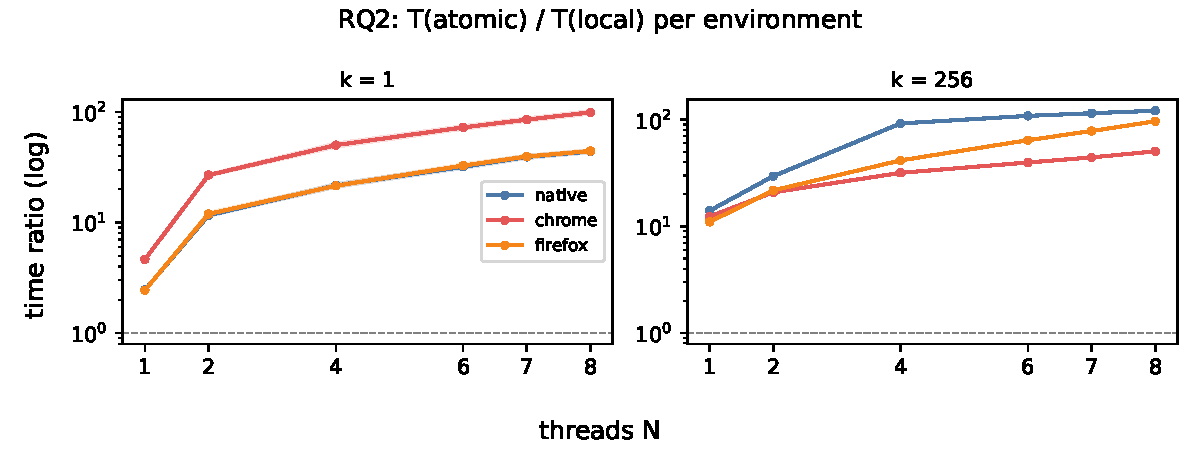
\includegraphics[width=0.8\linewidth]{../figures/campaign-rq2-ends.pdf}
\caption{RQ2: $T_{\mathrm{atomic}}/T_{\mathrm{local}}$ against $N$ at the
two ends of the sweep (log scale, 95\% CI).}
\Description{Atomic over local time ratio against thread count at k = 1 and k = 256, per environment.}
\label{fig:rq2-ends}
\end{figure}

\begin{figure}[htbp]
\centering
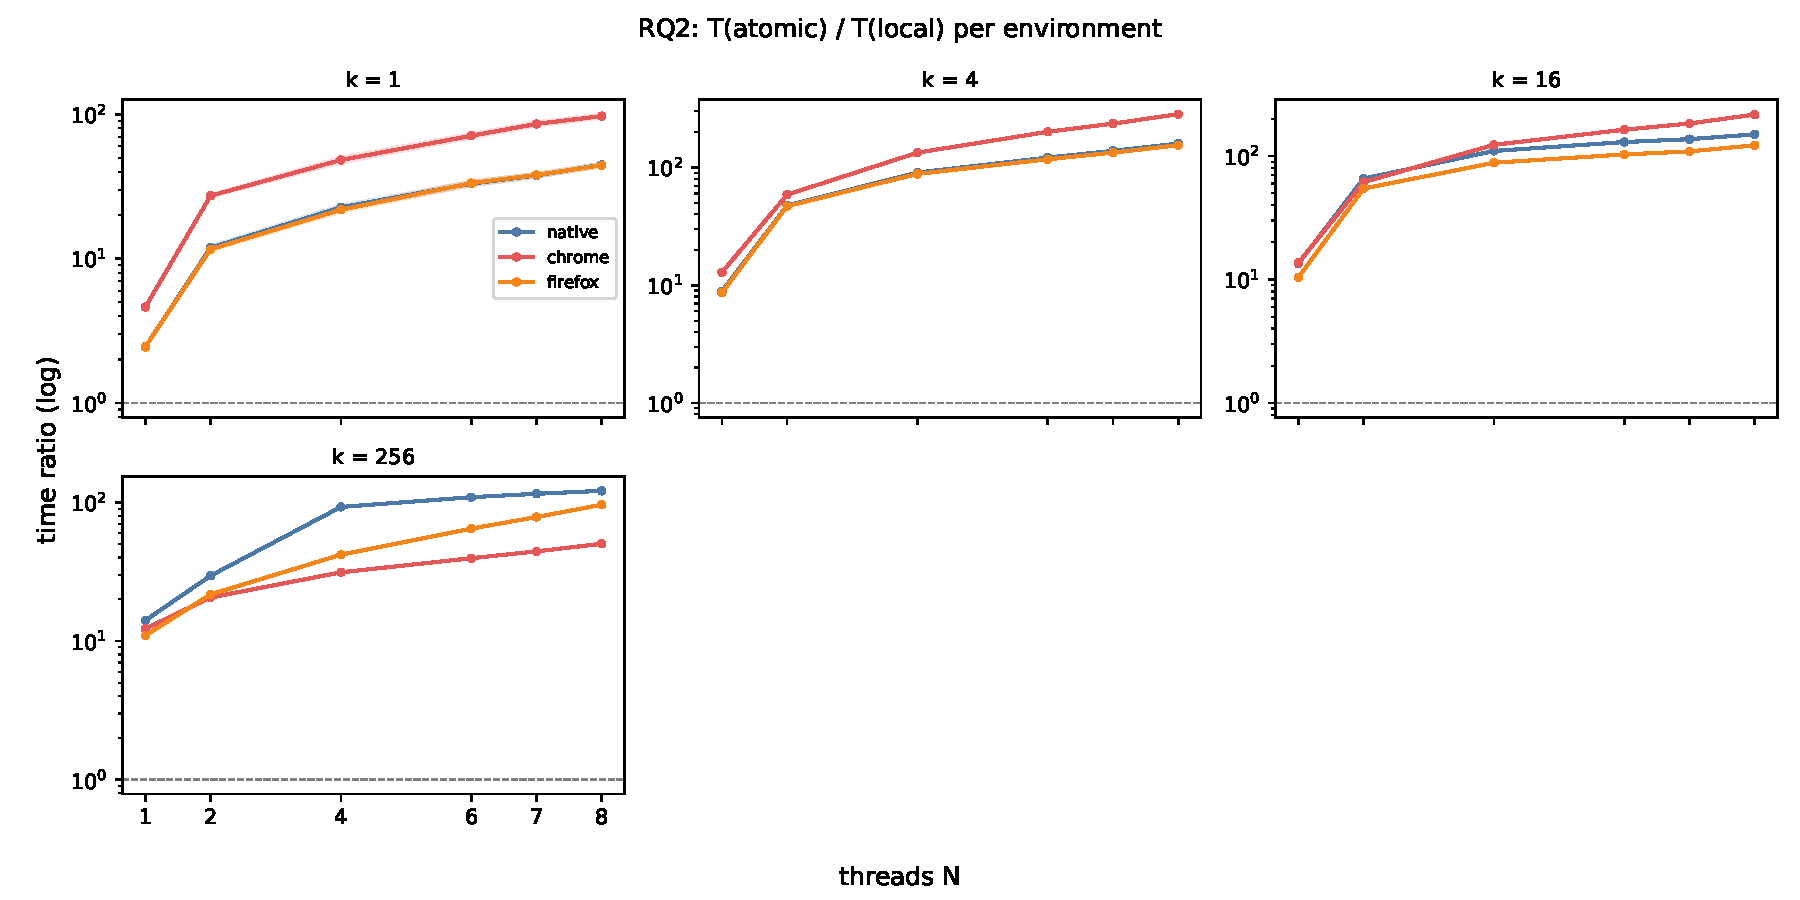
\includegraphics[width=\linewidth]{../figures/campaign-rq2.pdf}
\caption{RQ2: $T_{\mathrm{atomic}}/T_{\mathrm{local}}$ against $N$ for the
four values of $k$.}
\Description{Atomic over local time ratio against thread count for k = 1, 4, 16 and 256, per environment.}
\label{fig:rq2}
\end{figure}

\subsection{Every \texorpdfstring{$N$}{N}}

Table~\ref{tab:rq2-all} gives $\exp(\Delta r)$ for every thread count
(exploratory). Two things stand out. Part of Chrome's penalty exists
already with one thread: 1.89 at $k=1$ and 1.45 at $k=4$ with $N=1$, where
nothing is contended. At $k=1$ the atomic/local time ratio on one thread is
4.6 in Chrome against 2.5 natively and 2.4 in Firefox. So Chrome's effect
is a cost per operation as well as a cost of contention, which is what
Section~\ref{sec:why-rq2} finds in the machine code. And at $k=256$ both
browsers fall below 1 as soon as there are two threads, most at $N=4$
(Chrome 0.34, Firefox 0.45), because native code is at its worst there
(speedup 0.59 at $N=4$, Table~\ref{tab:speedup}).

\begin{table}[htbp]
\caption{Main campaign: the RQ2 effect $\exp(\Delta r)$ for every $k$ and $N$, with its 95\,\% bootstrap interval. Only $N=8$ is primary.}\label{tab:rq2-all}
\centering\small
\begin{tabular}{llcc}
\toprule
$k$ & $N$ & Chrome & Firefox \\
\midrule
1 & 1 & 1.89 [1.889, 1.891] & 0.9957 [0.9956, 0.9959] \\
1 & 2 & 2.313 [2.246, 2.379] & 1.029 [0.9891, 1.071] \\
1 & 4 & 2.319 [2.19, 2.461] & 0.9943 [0.9472, 1.043] \\
1 & 6 & 2.272 [2.16, 2.391] & 1.027 [0.9779, 1.076] \\
1 & 7 & 2.176 [2.072, 2.284] & 1.008 [0.9661, 1.053] \\
1 & 8 & 2.259 [2.157, 2.365] & 1.01 [0.9724, 1.049] \\
\midrule
4 & 1 & 1.45 [1.447, 1.454] & 0.977 [0.9763, 0.9777] \\
4 & 2 & 1.264 [1.244, 1.284] & 0.993 [0.9777, 1.009] \\
4 & 4 & 1.473 [1.457, 1.49] & 0.978 [0.9663, 0.9903] \\
4 & 6 & 1.651 [1.635, 1.669] & 0.96 [0.9493, 0.971] \\
4 & 7 & 1.722 [1.705, 1.739] & 0.9777 [0.9669, 0.9881] \\
4 & 8 & 1.771 [1.754, 1.787] & 0.9691 [0.9597, 0.9788] \\
\midrule
16 & 1 & 1.034 [1.031, 1.038] & 0.786 [0.7839, 0.7881] \\
16 & 2 & 0.9486 [0.9385, 0.959] & 0.8446 [0.8355, 0.8538] \\
16 & 4 & 1.14 [1.126, 1.154] & 0.8189 [0.8071, 0.8306] \\
16 & 6 & 1.266 [1.256, 1.277] & 0.7989 [0.792, 0.806] \\
16 & 7 & 1.344 [1.33, 1.359] & 0.8 [0.7932, 0.8067] \\
16 & 8 & 1.425 [1.408, 1.442] & 0.8311 [0.824, 0.8385] \\
\midrule
256 & 1 & 0.881 [0.8732, 0.8857] & 0.786 [0.771, 0.7966] \\
256 & 2 & 0.7061 [0.6995, 0.7103] & 0.7359 [0.7266, 0.7439] \\
256 & 4 & 0.3442 [0.341, 0.3473] & 0.4502 [0.445, 0.4553] \\
256 & 6 & 0.3654 [0.3613, 0.37] & 0.5918 [0.5861, 0.5979] \\
256 & 7 & 0.3852 [0.3823, 0.388] & 0.681 [0.6755, 0.6865] \\
256 & 8 & 0.4159 [0.4096, 0.4222] & 0.7965 [0.7864, 0.8058] \\
\bottomrule
\end{tabular}
\end{table}


\subsection{The two factors of the ratio}
\label{sec:decomposition}

$\exp(\Delta r)$ is a ratio of ratios:
\[
\exp(\Delta r) = \frac{A_b/A_n}{L_b/L_n},
\]
with $A$ the time of the atomic histogram, $L$ of the local one, $b$ a
browser and $n$ native. At $N=8$ the local kernel is about 1\% of the
atomic time, yet its own environment gap $L_b/L_n$ divides the result with
full weight: a browser whose local kernel is slower than native's gets a
lower $\exp(\Delta r)$ even if its atomics cost exactly what native's do.
The ratio is therefore always read with its two factors
(Table~\ref{tab:decomposition}), which tell the two engines apart.

\begin{table}[htbp]
\caption{The two factors of each primary RQ2 ratio at $N=8$ (post hoc, 95\,\% intervals): the atomic time and the local time in the browser over native, and the ratio of the excesses $(A_b-L_b)/(A_n-L_n)$.}\label{tab:decomposition}
\centering\footnotesize
\begin{tabular}{llcccc}
\toprule
Browser & $k$ & $\exp(\Delta r)$ & Atomic $A_b/A_n$ & Local $L_b/L_n$ & Excess \\
\midrule
Chrome & 1 & 2.259 [2.157, 2.365] & 2.206 [2.105, 2.308] & 0.9762 [0.9755, 0.977] & 2.234 [2.131, 2.34] \\
Chrome & 4 & 1.771 [1.754, 1.787] & 1.909 [1.892, 1.925] & 1.078 [1.074, 1.082] & 1.914 [1.897, 1.93] \\
Chrome & 16 & 1.425 [1.408, 1.442] & 1.78 [1.772, 1.788] & 1.249 [1.235, 1.264] & 1.784 [1.775, 1.792] \\
Chrome & 256 & 0.4159 [0.4096, 0.4222] & 0.5074 [0.5068, 0.508] & 1.22 [1.202, 1.239] & 0.5015 [0.5009, 0.5021] \\
Firefox & 1 & 1.01 [0.9724, 1.049] & 1.026 [0.9875, 1.066] & 1.015 [1.014, 1.017] & 1.026 [0.9868, 1.067] \\
Firefox & 4 & 0.9691 [0.9597, 0.9788] & 0.9837 [0.9751, 0.9926] & 1.015 [1.011, 1.019] & 0.9835 [0.9748, 0.9925] \\
Firefox & 16 & 0.8311 [0.824, 0.8385] & 1.007 [1.002, 1.013] & 1.212 [1.204, 1.22] & 1.006 [1.001, 1.011] \\
Firefox & 256 & 0.7965 [0.7864, 0.8058] & 0.9479 [0.9468, 0.949] & 1.19 [1.176, 1.205] & 0.9459 [0.9448, 0.947] \\
\bottomrule
\end{tabular}
\end{table}


\begin{itemize}[leftmargin=1.5em]
\item \emph{Chrome's effect is in the numerator.} Its atomic histogram
takes 2.21, 1.91 and 1.78 times the native time at $k=1$, 4 and 16, and
0.51 times at $k=256$; its local kernel is within 0.98 to 1.25 of native.
$\exp(\Delta r)$ falls from 2.26 to 1.43 between $k=1$ and 16 mostly
because Chrome's local kernel gets slower relative to native as $k$ grows,
while the atomic ratio stays near 2.
\item \emph{Firefox's effect is in the denominator.} Its atomic times are
the native ones (1.03, 0.98, 1.01 and 0.95 times) and its local histogram
is 1.21 and 1.19 times slower at $k=16$ and 256. ``Synchronization is
relatively cheaper in Firefox'' at $k \geq 16$ is true of the ratio and
misleading as a statement about synchronization.
\end{itemize}
The last column answers RQ2 in absolute terms, the time the shared counters
add in the browser over the time they add natively: about 2.2, 1.9 and 1.8
times in Chrome at $k \leq 16$ and 0.50 times at $k=256$; in Firefox 1.03,
0.98, 1.01 and 0.95. The two readings tell the same story for Chrome. For
Firefox they differ most at $k=16$: 0.83 by the ratio, 1.006 [1.001, 1.011]
by the excess.

\subsection{Robustness and sensitivity}

\begin{table}[htbp]
\caption{Robustness of the ten primary contrasts: Mann-Whitney $U$ and Cliff's $\delta$ on per-run ratios, Holm-adjusted, the share of 1000 random re-pairings with the same decision, and the agreement with the bootstrap decision.}\label{tab:robustness}
\centering\footnotesize
\begin{tabular}{lllrrrrlrl}
\toprule
RQ & Browser & Cell & $\delta$ & $U$ & $p$ & Holm $p$ & Rej. & Share & Agree \\
\midrule
RQ2 & Chrome & atomic, $k$=1 & 1 & 900 & 3.02e-11 & 3.02e-10 & yes & 1 & yes \\
RQ2 & Chrome & atomic, $k$=4 & 1 & 900 & 3.02e-11 & 3.02e-10 & yes & 1 & yes \\
RQ2 & Chrome & atomic, $k$=16 & 1 & 900 & 3.02e-11 & 3.02e-10 & yes & 1 & yes \\
RQ2 & Chrome & atomic, $k$=256 & -1 & 0 & 3.02e-11 & 3.02e-10 & yes & 1 & yes \\
RQ2 & Firefox & atomic, $k$=1 & 0.05778 & 476 & 0.7062 & 0.7062 & no & 1 & yes \\
RQ2 & Firefox & atomic, $k$=4 & -0.74 & 117 & 8.841e-07 & 2.652e-06 & yes & 1 & yes \\
RQ2 & Firefox & atomic, $k$=16 & -1 & 0 & 3.02e-11 & 3.02e-10 & yes & 1 & yes \\
RQ2 & Firefox & atomic, $k$=256 & -1 & 0 & 3.02e-11 & 3.02e-10 & yes & 1 & yes \\
RQ1 & Chrome & filter & -0.2444 & 340 & 0.1055 & 0.2109 & no & 0.999 & yes \\
RQ1 & Firefox & filter & 0.9244 & 866 & 8.097e-10 & 3.239e-09 & yes & 1 & yes \\
\bottomrule
\end{tabular}
\end{table}

\begin{table}[htbp]
\caption{The plan's sensitivity checks on the ten primary contrasts (effect with its 99.5\,\% interval): as planned, with the per-run mean, with the median across runs, and with no foreign-CPU exclusion. A decision that changes under a check would be marked not robust.}\label{tab:sensitivity}
\centering\footnotesize
\begin{tabular}{llcccl}
\toprule
Browser & Cell & As planned & Per-run mean & Median centre & Robust \\
\midrule
Chrome & atomic, $k$=1 & 2.259 [2.11, 2.406] & 2.259 [2.111, 2.406] & 2.397 [1.989, 2.512] & yes \\
Chrome & atomic, $k$=4 & 1.771 [1.746, 1.793] & 1.765 [1.736, 1.795] & 1.766 [1.741, 1.798] & yes \\
Chrome & atomic, $k$=16 & 1.425 [1.399, 1.451] & 1.429 [1.397, 1.461] & 1.419 [1.4, 1.452] & yes \\
Chrome & atomic, $k$=256 & 0.4159 [0.4072, 0.4251] & 0.4158 [0.4066, 0.4256] & 0.4146 [0.4028, 0.4279] & yes \\
Firefox & atomic, $k$=1 & 1.01 [0.9573, 1.067] & 0.994 [0.9408, 1.049] & 1.053 [0.9509, 1.111] & yes \\
Firefox & atomic, $k$=4 & 0.9691 [0.9555, 0.9827] & 0.9727 [0.9577, 0.9885] & 0.9671 [0.9512, 0.9854] & yes \\
Firefox & atomic, $k$=16 & 0.8311 [0.8208, 0.8417] & 0.8385 [0.825, 0.8525] & 0.83 [0.8155, 0.8458] & yes \\
Firefox & atomic, $k$=256 & 0.7965 [0.782, 0.8089] & 0.7992 [0.7821, 0.8139] & 0.8046 [0.7862, 0.8177] & yes \\
Chrome & filter & 0.9955 [0.9868, 1.004] & 0.9936 [0.984, 1.003] & 0.9953 [0.9807, 1.009] & yes \\
Firefox & filter & 1.055 [1.034, 1.072] & 1.037 [1.015, 1.055] & 1.051 [1.037, 1.071] & yes \\
\bottomrule
\end{tabular}
\end{table}


Mann-Whitney agrees with the bootstrap decision on all ten primary
contrasts (Table~\ref{tab:robustness}). The eight rejected ones have
$|\delta| \geq 0.74$, six of them $|\delta| = 1$: every browser run is on
one side of every native run. The two not rejected have $p = 0.11$ (Chrome,
RQ1) and $p = 0.71$ (Firefox, $k=1$). The decision is the same in at least
99.9\% of 1000 random re-pairings of the runs. All ten decisions also hold
under the plan's three sensitivity checks (Table~\ref{tab:sensitivity}):
the per-run mean, the median across runs (which widens Chrome's interval at
$k=1$ to [1.99, 2.51], the cell whose runs fall on levels) and no exclusion
threshold (identical, since no run was excluded).

\section{What Explains the Results}
\label{sec:why}

The main campaign gives two findings that need an explanation: the filter
scales better in Firefox than natively (RQ1), and Chrome's shared atomics
cost more than native ones at small $k$ and less at $k=256$ (RQ2). After
the main campaign and before the campaigns and probes that test them, nine
questions were written down, each with its hypothesis, its test and what
the test would show if the hypothesis held and if it did not
(Table~\ref{tab:questions}). Nothing in this section is a primary result:
it supports or weakens an explanation of one.

\begin{table}[htbp]
\caption{The nine questions, written before their tests, and how each
ended. \emph{Answered}: an intervention that changes one thing reproduces
the effect. \emph{Supported}: independent observations agree with the
prediction. \emph{Open}: not explained.}
\label{tab:questions}
\centering\scriptsize
\begin{tabular}{rp{0.22\linewidth}p{0.24\linewidth}p{0.17\linewidth}p{0.22\linewidth}}
\toprule
\# & What is seen & Hypothesis & Tested by & Outcome \\
\midrule
1 & The filter's efficiency is 0.87 at $N=8$ natively and in Chrome & At eight threads the filter is bound by memory, not by the cores & Counters of the loop, SIMD builds, image sizes & Supported, for about half of the loss natively \\
2 & Firefox's filter scales better (0.917) with a slower thread & Slower code per thread asks less of the shared memory & The same three, and the engine arms & Supported \\
3 & At $N=1$ the filter takes 1.36 times the native time in Firefox, 1.17 in Chrome & The engines' code for the same WASM is longer or slower & Counters of the loop, the machine code & Answered as far as counters go: a third more instructions \\
4 & The local histogram's efficiency dips at $N=6$ and 7 & Rayon splits in powers of two, which loads six or seven threads unevenly & Fixed grains at $N=6$, 7, 8 & Not supported; open \\
5 & The local histogram's speedup passes 8 in Firefox & One thread pays for cache misses that eight do not & Counters of the loop & Supported \\
6 & With one thread, Chrome's atomic time depends on $k$; native and Firefox do not & V8's optimizing compiler emits a load and a compare-and-swap, a chain through memory & Engine arms, machine code, native probe & Answered \\
7 & At $k=256$, $N=8$ Chrome's atomic histogram is twice as fast as native & The same sequence changes how eight cores contend for 256 lines & Engine arms, native probe & Answered for the sequence; the mechanism is open \\
8 & Firefox's RQ2 ratio is under 1 at $k=16$ and 256 & It comes from the denominator: its local histogram scales more & The two factors of the ratio & Shown by the times; its cause is question 5 \\
9 & The atomic cells at $k=1$ fall on several time levels & The levels are states of contention that differ from run to run & Counters per run & Supported \\
\bottomrule
\end{tabular}
\end{table}

\paragraph{What the tests can show.} The native probe changes one thing, the
instructions of the increment, and looks at the effect: it is the test that
can show a cause. The engine arms change the whole compiler, so every
instruction of the loop changes with the increment; they show that an
effect follows the compiler. Counters, image sizes and SIMD builds give
correlations: several sources that agree support an explanation, and none
of them is an intervention on what the filter asks of the memory.

\subsection{The machine code}
\label{sec:engine-code}

We captured the machine code that runs each kernel: LLVM's from the native
binary, the WASM both browsers receive, V8's from a diagnostic run in which
it writes its compiled code (for both of its compilers), and
SpiderMonkey's by sampling a long run with \code{perf} and reading the
sampled pages of its code from the process memory (its release build writes
no dump; the bytes were read twice, five seconds apart, and had to be
equal). LLVM unrolls alike for both targets: eight atomic increments per
turn and four plain ones, in x86 and in WASM. What differs between native
and browser is made by the engine from the same WASM.

\begin{figure}[htbp]
\footnotesize
\begin{minipage}[t]{0.47\linewidth}
\textbf{LLVM, native}
\begin{verbatim}
movzbl (%r8),%r9d
shl    $0x7,%r9d
lock incq (%rsi,%r9,1)
\end{verbatim}
\textbf{SpiderMonkey, optimizing}
\begin{verbatim}
movzbl (%r15,%rdi,1),%r8d
shl    $0x7,%r8d
add    %ebx,%r8d
test   $0x7,%r8b      ; alignment
jne    <trap>
mov    $0x1,%r9d
lock add %r9,(%r15,%r8,1)
\end{verbatim}
\end{minipage}\hfill
\begin{minipage}[t]{0.47\linewidth}
\textbf{V8, optimizing (TurboFan)}
\begin{verbatim}
movzbl (%rdi,%rsi,1),%r8d
shl    $0x7,%r8d
add    %r15d,%r8d
...                   ; alignment
mov    $0x1,%r11d
mov    (%rdi,%r8,1),%rax   ; load
mov    %rax,%rcx
add    %r11,%rcx           ; add
lock cmpxchg %rcx,(%rdi,%r8,1)
jne    <back to the load>  ; retry
\end{verbatim}
\textbf{V8, baseline (Liftoff)}
\begin{verbatim}
...             ; alignment, bounds
lock xadd %rcx,(%r12,%rax,1)
\end{verbatim}
\end{minipage}
\caption{One atomic increment of the shared histogram, as each compiler
emits it for the same \code{i64.atomic.rmw.add} (the first of the eight
increments of a loop turn, from the captured listings; comments added).}
\Description{Four short assembly listings: lock inc for LLVM, lock add for SpiderMonkey, a load, add and lock cmpxchg with a retry jump for V8's optimizing compiler, and lock xadd for V8's baseline compiler.}
\label{fig:listings}
\end{figure}

\begin{itemize}[leftmargin=1.5em]
\item \emph{Atomic increment} (Figure~\ref{fig:listings}). LLVM emits one
\code{lock inc}. SpiderMonkey emits one \code{lock add} behind an alignment
check. V8's optimizing compiler emits a load, an add and a \code{lock
cmpxchg} that jumps back to the load until it succeeds: a compare-and-swap
loop, for an add whose result the program does not use. V8's baseline
compiler emits a \code{lock xadd} behind an alignment check and a bounds
check.
\item \emph{Plain increment} (the local histogram). LLVM: \code{inc} on
memory, four per turn. Both engines: a load, an add and a store.
\item \emph{Filter.} LLVM: SSE2 in legacy encoding, 65 instructions for 16
pixels. V8 optimizing: the same 128-bit operations in VEX encoding, with one
SSE4.1 operation, 87 instructions. SpiderMonkey: a mix of VEX-encoded and
legacy-encoded vector instructions, with \code{palignr}, 85 instructions.
That is 4.06, 5.44 and 5.31 instructions per pixel.
\end{itemize}
A listing says which instructions run, not how long each takes. The Chrome
listings come from diagnostic runs with flags that no campaign uses, at a
smaller size; that the code is the one a campaign runs is assumed.
SpiderMonkey's baseline code was not captured.

\subsection{RQ2: one instruction sequence}
\label{sec:why-rq2}

\begin{figure}[htbp]
\centering
\begin{tikzpicture}[font=\scriptsize, x=1cm, y=1cm,
  step/.style={draw, rounded corners=1pt, minimum height=5mm, inner sep=2pt},
  arr/.style={-{Stealth[length=1.6mm]}}]
  \node[font=\footnotesize\bfseries, anchor=west] at (0,2.6) {Locked add (LLVM, SpiderMonkey)};
  \node[step, fill=native!15] (a1) at (1.2,1.8) {take line exclusive};
  \node[step, fill=native!15, right=3mm of a1] (a2) {add 1};
  \node[step, fill=native!15, right=3mm of a2] (a3) {done};
  \draw[arr] (a1) -- (a2); \draw[arr] (a2) -- (a3);
  \node[anchor=west, text width=5.4cm] at (0,1.0) {One transfer of the line per increment. Never repeated.};
  \node[font=\footnotesize\bfseries, anchor=west] at (6.6,2.6) {Compare-and-swap loop (V8 optimizing)};
  \node[step, fill=chrome!15] (b1) at (7.4,1.8) {load value};
  \node[step, fill=chrome!15, right=3mm of b1] (b2) {add 1};
  \node[step, fill=chrome!15, right=3mm of b2] (b3) {\code{lock cmpxchg}};
  \node[step, fill=chrome!15, right=3mm of b3] (b4) {done};
  \draw[arr] (b1) -- (b2); \draw[arr] (b2) -- (b3); \draw[arr] (b3) -- node[above]{same} (b4);
  \draw[arr] (b3.south) -- ++(0,-4mm) -| node[pos=0.25, below]{value changed by another core: retry} (b1.south);
  \node[anchor=west, text width=6.6cm] at (6.6,0.35) {A read of the line, then a write. If another core wrote in between, everything is done again.};
\end{tikzpicture}
\caption{The two ways an atomic add is compiled. Under concentrated
contention the right-hand sequence is retried once every four adds
(Table~\ref{tab:retries}).}
\Description{Two diagrams: a locked add that takes the line and adds, and a compare-and-swap loop that loads, adds, tries a locked compare-and-swap and retries when another core changed the value.}
\label{fig:cas}
\end{figure}

\paragraph{Prediction.} If the cause of Chrome's RQ2 effect is the sequence
of Figure~\ref{fig:cas}, then (a) Chrome with its baseline compiler only,
which emits a \code{lock xadd}, should not depend on $k$ with one thread
and should lose the advantage at $k=256$; and (b) a native program with the
compare-and-swap sequence should be slower at $k=1$ and faster at $k=256$
with eight threads.

\paragraph{The engine arms.} The tier campaign (2100 runs) ran each browser
as shipped, with its optimizing compiler only and with its baseline
compiler only, for the filter and both histograms at $k=1$ and 256, $N=1$
and 8 (Table~\ref{tab:tier}). In every cell of both browsers the arm as
shipped and the optimizing-only arm give the same time after the warm-up
(Chrome's atomic histogram at $k=1$ with one thread: 697.97 and 697.98~ms):
\emph{the campaigns measure the optimizing compiler}. The baseline-only arm
differs everywhere. With one thread, Chrome's atomic time is 698~ms at
$k=1$ and 412~ms at $k=256$ with the optimizing compiler, and 419 and
403~ms with the baseline one: the dependence on $k$ follows the optimizing
compiler, as predicted. The RQ2 effect at $k=1$ follows: 2.17 with the
optimizing compiler, 1.04 with the baseline one. With its baseline compiler
Chrome pays for the shared counter at $k=1$ what native code pays.

{\small
\begin{longtable}{lllrrcr}
\caption{Engine arms (tier campaign, 2100 runs): each browser as shipped (default), with its optimizing compiler only and with its baseline compiler only. Time in ms at $N=1$ and 8, speedup at $N=8$ with its 95\,\% interval, and the first warm-up iteration over the run's value at $N=1$.}\label{tab:tier} \\
\toprule
Workload & Environment & Arm & $T_1$ & $T_8$ & $S_8$ [95\,\%] & First it. \\
\midrule
\endfirsthead
\toprule
Workload & Environment & Arm & $T_1$ & $T_8$ & $S_8$ [95\,\%] & First it. \\
\midrule
\endhead
\bottomrule
\endfoot
filter & Native &  & 22.597 & 3.259 & 6.933 [6.919, 6.947] & 2.005 \\
filter & Chrome & default & 26.674 & 3.839 & 6.948 [6.878, 7.06] & 1.027 \\
filter & Chrome & optimizing & 26.494 & 3.877 & 6.833 [6.798, 6.868] & 1.436 \\
filter & Chrome & baseline & 32.080 & 4.523 & 7.093 [7.06, 7.127] & 1.012 \\
filter & Firefox & default & 30.799 & 4.178 & 7.372 [7.295, 7.45] & 1.012 \\
filter & Firefox & optimizing & 31.185 & 4.192 & 7.44 [7.333, 7.546] & 1.002 \\
filter & Firefox & baseline & 39.124 & 5.206 & 7.515 [7.454, 7.575] & 1.001 \\
\midrule
atomic, $k$=1 & Native &  & 379.6 & 857.2 & 0.4429 [0.43, 0.4563] & 1.001 \\
atomic, $k$=1 & Chrome & default & 698.0 & 1835.0 & 0.3804 [0.3675, 0.3936] & 0.9486 \\
atomic, $k$=1 & Chrome & optimizing & 698.0 & 1823.2 & 0.3828 [0.3701, 0.3956] & 1.014 \\
atomic, $k$=1 & Chrome & baseline & 419.0 & 898.4 & 0.4665 [0.4532, 0.4798] & 1.001 \\
atomic, $k$=1 & Firefox & default & 379.7 & 853.9 & 0.4447 [0.4326, 0.4568] & 1.007 \\
atomic, $k$=1 & Firefox & optimizing & 379.7 & 874.2 & 0.4343 [0.4205, 0.4484] & 1 \\
atomic, $k$=1 & Firefox & baseline & 411.3 & 896.7 & 0.4587 [0.4469, 0.4714] & 1 \\
\midrule
atomic, $k$=256 & Native &  & 379.6 & 414.0 & 0.9168 [0.9158, 0.9177] & 1.001 \\
atomic, $k$=256 & Chrome & default & 411.9 & 210.3 & 1.958 [1.957, 1.959] & 0.9993 \\
atomic, $k$=256 & Chrome & optimizing & 411.9 & 210.3 & 1.958 [1.957, 1.959] & 1.024 \\
atomic, $k$=256 & Chrome & baseline & 402.7 & 270.1 & 1.491 [1.49, 1.492] & 1.001 \\
atomic, $k$=256 & Firefox & default & 379.8 & 392.9 & 0.9668 [0.9662, 0.9674] & 1.002 \\
atomic, $k$=256 & Firefox & optimizing & 379.8 & 393.1 & 0.9662 [0.9658, 0.9666] & 1 \\
atomic, $k$=256 & Firefox & baseline & 384.0 & 326.5 & 1.176 [1.176, 1.177] & 1.001 \\
\midrule
local, $k$=1 & Native &  & 154.9 & 19.475 & 7.956 [7.951, 7.959] & 1.002 \\
local, $k$=1 & Chrome & default & 150.7 & 19.004 & 7.929 [7.922, 7.936] & 1.007 \\
local, $k$=1 & Chrome & optimizing & 150.5 & 19.082 & 7.888 [7.874, 7.9] & 1.075 \\
local, $k$=1 & Chrome & baseline & 154.5 & 19.638 & 7.867 [7.855, 7.878] & 1.005 \\
local, $k$=1 & Firefox & default & 155.7 & 19.785 & 7.867 [7.858, 7.876] & 1.005 \\
local, $k$=1 & Firefox & optimizing & 155.7 & 19.788 & 7.866 [7.858, 7.874] & 1.002 \\
local, $k$=1 & Firefox & baseline & 150.8 & 19.143 & 7.876 [7.867, 7.885] & 1.002 \\
\midrule
local, $k$=256 & Native &  & 27.058 & 3.425 & 7.901 [7.874, 7.926] & 1.021 \\
local, $k$=256 & Chrome & default & 33.624 & 4.194 & 8.017 [7.88, 8.164] & 1.11 \\
local, $k$=256 & Chrome & optimizing & 33.486 & 4.091 & 8.184 [8.073, 8.312] & 1.342 \\
local, $k$=256 & Chrome & baseline & 53.921 & 6.979 & 7.726 [7.615, 7.84] & 1.012 \\
local, $k$=256 & Firefox & default & 34.411 & 4.090 & 8.413 [8.28, 8.568] & 1.122 \\
local, $k$=256 & Firefox & optimizing & 34.074 & 4.052 & 8.409 [8.323, 8.487] & 1.016 \\
local, $k$=256 & Firefox & baseline & 54.435 & 6.686 & 8.142 [7.861, 8.541] & 1.008 \\
\end{longtable}
}


\paragraph{The native probe.} A native C program counts into the bench's
table (256 counters, 128 bytes apart) on the bench's input, with 1 or 8
threads each pinned to one P-core and given one slice of the image. Only
the instructions of one increment change between its five sequences
(Table~\ref{tab:probe}).

\begin{table}[htbp]
\caption{Native atomic-increment probe: median time of a pass in ms over 10 timed passes, by increment sequence. Only the instructions of the increment change between rows.}\label{tab:probe}
\centering\small
\begin{tabular}{lrrrrrr}
\toprule
Sequence & $k$=1, $N$=1 & $k$=1, $N$=8 & $k$=16, $N$=1 & $k$=16, $N$=8 & $k$=256, $N$=1 & $k$=256, $N$=8 \\
\midrule
\texttt{lock-inc} & 379.9 & 976.2 & 379.8 & 550.1 & 379.8 & 415.0 \\
\texttt{compare-and-swap} & 677.1 & 2131.8 & 484.9 & 1018.9 & 408.2 & 239.5 \\
\texttt{lock-xadd} & 382.6 & 975.3 & 380.7 & 547.1 & 380.3 & 437.2 \\
\texttt{lock-inc-checked} & 381.6 & 972.9 & 380.3 & 556.1 & 380.0 & 401.6 \\
\texttt{lock-xadd-checked} & 392.4 & 983.9 & 383.5 & 556.4 & 380.2 & 348.8 \\
\bottomrule
\end{tabular}
\end{table}


\begin{itemize}[leftmargin=1.5em]
\item \emph{The prediction holds.} The compare-and-swap is 1.78 times the
locked increment at $k=1$ with one thread and 2.18 times with eight, and
0.58 times at $k=256$ with eight.
\item \emph{It gives Chrome's times.} Chrome's atomic histogram takes 698,
488 and 412~ms with one thread at $k=1$, 16 and 256; the compare-and-swap
gives 677, 485 and 408~ms, within 3\%. At $k=256$ with eight threads Chrome
takes 210~ms and the probe 240~ms, 14\% more.
\item \emph{The locked increment gives the native times}: 380~ms with one
thread at every $k$, 415~ms at $k=256$ with eight.
\end{itemize}
The engine arms show that the effect follows the compiler; the probe
isolates the increment. Together: the cost of Chrome's atomic histogram at
$k=1$ is the compare-and-swap sequence of V8's optimizing compiler
(question 6, answered). It costs more already with one thread because at
$k=1$ the loop becomes a chain through memory, each load waiting for the
previous locked write.

\paragraph{Retries, counted.} A separate campaign (720 runs) ran
\code{perf stat} on the P-cores during the runs
(Tables~\ref{tab:counters-atomic} and~\ref{tab:retries}). Each
compare-and-swap attempt is a locked load, so locked loads per add above
the one-thread count are retries. At $k=1$ with eight threads Chrome makes
0.242 more per add (95\% CI [0.225, 0.259]) against 0.001 natively and
0.002 in Firefox, which runs the same WASM module and the same pool: about
one add in four is retried. Chrome also reads the contended line from
another core before writing it (0.30 read HITMs per add at $k=1$, 0.71 at
$k=256$; under 0.01 elsewhere), which the load of its sequence explains.
At $k=256$ Chrome needs the line for writing from another core 0.52 times
per add where native code needs it 1.04 times and Firefox 0.89 times, and
takes 86 cycles per add against 158 and 164.

\begin{table}[htbp]
\caption{Hardware counters of the atomic histogram per atomic add (means of 30 runs, counted system-wide on the P-cores for the whole run): cycles, instructions, locked loads, lines taken for writing from another core (RFO HITM), lines read from another core (read HITM) and L2 misses.}\label{tab:counters-atomic}
\centering\small
\begin{tabular}{lllrrrrrr}
\toprule
$k$ & $N$ & Environment & Cycles & Instr. & Lock loads & RFO HITM & Read HITM & L2 miss. \\
\midrule
1 & 1 & Native & 19.1533 & 5.0767 & 0.9992 & 0.0000 & 0.0000 & 0.0008 \\
1 & 1 & Chrome & 37.7201 & 24.1086 & 1.0160 & 0.0006 & 0.0016 & 0.0069 \\
1 & 1 & Firefox & 31.4093 & 33.1235 & 1.0370 & 0.0018 & 0.0053 & 0.0195 \\
\midrule
1 & 8 & Native & 336.0000 & 5.5722 & 1.0003 & 0.2425 & 0.0002 & 0.2177 \\
1 & 8 & Chrome & 680.9191 & 26.7122 & 1.2582 & 0.1956 & 0.2992 & 0.3872 \\
1 & 8 & Firefox & 365.1023 & 34.1941 & 1.0391 & 0.2500 & 0.0058 & 0.2209 \\
\midrule
256 & 1 & Native & 19.1209 & 5.0697 & 0.9986 & 0.0000 & 0.0000 & 0.0006 \\
256 & 1 & Chrome & 25.9478 & 24.0954 & 1.0159 & 0.0006 & 0.0015 & 0.0065 \\
256 & 1 & Firefox & 32.4503 & 33.3375 & 1.0379 & 0.0018 & 0.0052 & 0.0196 \\
\midrule
256 & 8 & Native & 158.3065 & 5.3206 & 0.9990 & 1.0406 & 0.0001 & 0.8015 \\
256 & 8 & Chrome & 85.5763 & 24.5930 & 1.0305 & 0.5171 & 0.7117 & 0.2134 \\
256 & 8 & Firefox & 164.0309 & 33.8173 & 1.0388 & 0.8898 & 0.0057 & 0.7718 \\
\bottomrule
\end{tabular}
\end{table}

\begin{table}[htbp]
\caption{Locked loads per operation at $N=8$ above the one-thread count, with its 95\,\% interval. For the atomic histogram in Chrome each is a retried compare-and-swap.}\label{tab:retries}
\centering\small
\begin{tabular}{llccc}
\toprule
Workload &  & Native & Chrome & Firefox \\
\midrule
filter &  & 0.0004 [0.0003, 0.0005] & 0.0011 [0.0007, 0.0016] & 0.0001 [-0.0004, 0.0005] \\
atomic, $k$=1 &  & 0.0010 [0.0001, 0.0020] & 0.2422 [0.2251, 0.2588] & 0.0021 [0.0017, 0.0025] \\
atomic, $k$=256 &  & 0.0004 [-0.0008, 0.0017] & 0.0146 [0.0142, 0.0151] & 0.0008 [0.0003, 0.0014] \\
local, $k$=256 &  & 0.0003 [-0.0000, 0.0005] & 0.0014 [0.0011, 0.0017] & 0.0004 [0.0003, 0.0006] \\
\bottomrule
\end{tabular}
\end{table}


\paragraph{The advantage at $k=256$: the sequence is enough, the mechanism
is open.} The probe's prediction held (240~ms against 415). The tier
campaign's held only in part: the baseline arm was expected to lose the
advantage over native and keeps most of it (270~ms), and Firefox's baseline
compiler gains one that its optimizing compiler does not have (327 against
393~ms). The probe shows the same for the baseline sequence: the
exchange-and-add behind an alignment and a bounds check takes 349~ms, while
the checks alone (402~ms) and the exchange-and-add alone (437~ms) do not
gain. So at $k=256$ with eight threads the time is not ordered by how fast
one increment is: the sequences that do more around the locked write finish
sooner. The explanation offered, and not tested, is that eight cores
hitting 256 lines at random spend their time moving lines between caches,
and a sequence that reads the line first, or does other work between two
locked writes, asks for exclusive ownership less often. The prediction that
failed in part is kept as such (question 7).

\paragraph{Limits of the probe.} Each thread has a fixed slice and a fixed
core, where the bench splits the image into Rayon tasks and leaves
placement to the kernel, so its eight-thread times at $k=1$ and 16 are not
the bench's (976 against 856~ms at $k=1$). One session, ten passes per
cell. It shows that the sequence is enough to produce the effect on this
CPU, which is less than showing that nothing else contributes to Chrome's
times.

\paragraph{What the arms show besides.} In the arm as shipped, the first
warm-up iteration of Chrome's atomic histogram at $k=1$ is 0.949 times the
steady value; with one compiler only it is 1.00 and 1.01. A run as shipped
starts in baseline code, which is the faster one for this loop: the warm-up
here ends in slower code, the opposite of the usual tier-up. And the RQ2
effect at $k=256$ does not read cleanly for the baseline arms (0.32 in
Chrome, 0.40 in Firefox), because the baseline compilers' local histogram
is much slower (7.0 against 4.2~ms in Chrome at eight threads) and the
effect divides by it: the times are the reading.

\subsection{RQ1: why the filter is slower in the browsers}
\label{sec:why-rq1}

\paragraph{Counters of the loop alone.} A counter of a whole browser run is
mostly not the loop: the first counters campaign gave 3.7 instructions per
pixel for the native local histogram, 12.6 in Chrome and 21.3 in Firefox,
where the loop itself is 2.75. So two campaigns were run that differ only
in the passes per timed sample, one and eight, counted the same way; a run
of the second does seven more passes of every timed sample than a run of
the first and nothing else differs (same start, same input, same checksums).
For each cell and counter,
\[
\frac{\overline{C}_{8\,\mathrm{passes}} - \overline{C}_{1\,\mathrm{pass}}}{7 \times \mathrm{samples} \times \mathrm{pixels}}
\]
is the count per pixel of the loop alone, with an interval from a bootstrap
over the runs of both campaigns (10 runs each per cell). The check that the
difference works: the native local histogram at one thread gives 2.77
[2.76, 2.79] instructions per pixel against the 2.75 of its code.
Table~\ref{tab:counters-loop} has the result. The two campaigns ran one
after the other, 25 minutes apart, so the pass count is confounded with the
block; a count of instructions does not drift as a time does, but cycles
and misses could.

\begin{table}[htbp]
\caption{Counters of the loop alone at one thread, per pixel, by the difference of two pass counts (10 runs with one pass and 10 with eight), with 95\,\% bootstrap intervals. LLC and L2 are cache misses.}\label{tab:counters-loop}
\centering\scriptsize
\resizebox{\linewidth}{!}{%
\begin{tabular}{llcccc}
\toprule
Workload & Environment & Instructions & Cycles & LLC misses & L2 misses \\
\midrule
filter & Native & 4.103 [4.098, 4.108] & 1.067 [1.062, 1.072] & 0.01378 [0.01374, 0.01383] & 0.000329 [0.0003247, 0.0003335] \\
filter & Chrome & 5.517 [5.478, 5.539] & 1.243 [1.221, 1.26] & 0.01285 [0.01277, 0.01292] & 0.0003967 [0.0003883, 0.0004042] \\
filter & Firefox & 5.408 [5.371, 5.431] & 1.451 [1.428, 1.473] & 0.01049 [0.01034, 0.01064] & 0.000424 [0.0004113, 0.0004354] \\
\midrule
local, $k$=16 & Native & 2.761 [2.755, 2.767] & 1.359 [1.356, 1.363] & 0.003641 [0.003621, 0.003661] & 0.0004206 [0.0004167, 0.0004239] \\
local, $k$=16 & Chrome & 7.025 [7.02, 7.03] & 1.708 [1.699, 1.718] & 0.003774 [0.003697, 0.003856] & 0.0004188 [0.0004122, 0.0004257] \\
local, $k$=16 & Firefox & 6.819 [6.814, 6.825] & 1.751 [1.745, 1.755] & 0.003558 [0.003474, 0.003644] & 0.0004669 [0.0004556, 0.0004786] \\
\midrule
local, $k$=256 & Native & 2.772 [2.761, 2.785] & 1.294 [1.288, 1.3] & 0.004266 [0.004236, 0.004299] & 0.0004456 [0.00044, 0.0004517] \\
local, $k$=256 & Chrome & 7.004 [6.978, 7.025] & 1.593 [1.564, 1.637] & 0.00307 [0.002981, 0.00317] & 0.0004338 [0.0004246, 0.0004416] \\
local, $k$=256 & Firefox & 6.817 [6.811, 6.822] & 1.701 [1.638, 1.819] & 0.003646 [0.003578, 0.003714] & 0.0004924 [0.0004735, 0.0005083] \\
\bottomrule
\end{tabular}
}
\end{table}


\paragraph{Question 3: a third more instructions.} With one thread the
filter runs 4.10 instructions per pixel natively, 5.52 in Chrome and 5.41
in Firefox: both engines run about a third more instructions than native
code (1.34 and 1.32 times), and the listings give the same counts. Chrome
runs them at a higher rate (4.44 instructions per cycle against 3.84) and
ends at 1.17 times the native cycles; Firefox runs them at the native rate
or below (3.73) and ends at 1.36 times. Those two ratios are the time
ratios of the main campaign. Firefox's loop is as long as Chrome's and runs
slower; it mixes two encodings of vector instructions, and whether that is
why was not tested. The local histogram is the same in larger: 2.77
instructions per pixel natively against 7.0 in Chrome and 6.8 in Firefox,
for 1.23 and 1.31 times the cycles at $k=256$.

\subsection{RQ1: why the filter does not reach 8, and why Firefox comes closer}

\paragraph{Question 1: bound by memory.} The prediction for a loop bound by
memory at eight threads was: the same instructions per pixel as with one
thread, more cache misses, and about 1.15 times the cycles (the inverse of
the efficiency). The first two hold (Table~\ref{tab:counters-loop}): from
one to eight threads the instructions per pixel change by under 1\% in the
three environments and the last-level misses rise by 1.43, 1.47 and 1.25
times. The cycles rise by 8.5\% natively [7.6, 9.3], not 15\%: the cores'
own work per pixel explains about half of the lost efficiency. The rest is
time in which a core is not running the loop at all, which a counter of
cycles does not see; it fits the cost of handing out and collecting the
tasks and was not measured.

\paragraph{Question 2: a slower loop asks less.} The rise of the cycles
from one to eight threads is smaller in Firefox than natively, 1.032
[1.012, 1.054] against 1.085 [1.076, 1.093], the intervals apart, and its
last-level misses rise less. Two other sources agree.

\begin{table}[htbp]
\caption{SIMD variants of the filter: time in ms at $N=1$ and 8, megabytes read per second by one thread, efficiency at $N=8$ with its 95\,\% interval, the excess $T_8-T_1/8$ in \textmu s, and the time over native of the same build at $N=1$ and 8.}\label{tab:simd}
\centering\footnotesize
\begin{tabular}{llrrrcrrr}
\toprule
Build & Environment & $T_1$ & $T_8$ & MB/s & Eff.\ $N$=8 & Excess & /nat.\ 1 & /nat.\ 8 \\
\midrule
scalar & Native & 88.259 & 11.239 & 760 & 0.982 [0.979, 0.984] & 206.9 & 1.000 & 1.000 \\
scalar & Chrome & 130.3 & 16.861 & 515 & 0.966 [0.965, 0.967] & 569.0 & 1.477 & 1.500 \\
scalar & Firefox & 141.0 & 17.939 & 476 & 0.982 [0.982, 0.983] & 317.2 & 1.597 & 1.596 \\
baseline & Native & 22.601 & 3.249 & 2969 & 0.869 [0.868, 0.871] & 424.3 & 1.000 & 1.000 \\
baseline & Chrome & 26.486 & 3.825 & 2534 & 0.865 [0.861, 0.870] & 514.5 & 1.172 & 1.177 \\
baseline & Firefox & 30.808 & 4.200 & 2178 & 0.917 [0.904, 0.928] & 348.5 & 1.363 & 1.292 \\
avx2 & Native & 15.471 & 2.682 & 4338 & 0.721 [0.720, 0.722] & 748.3 & 1.000 & 1.000 \\
\bottomrule
\end{tabular}
\end{table}


\begin{figure}[htbp]
\centering
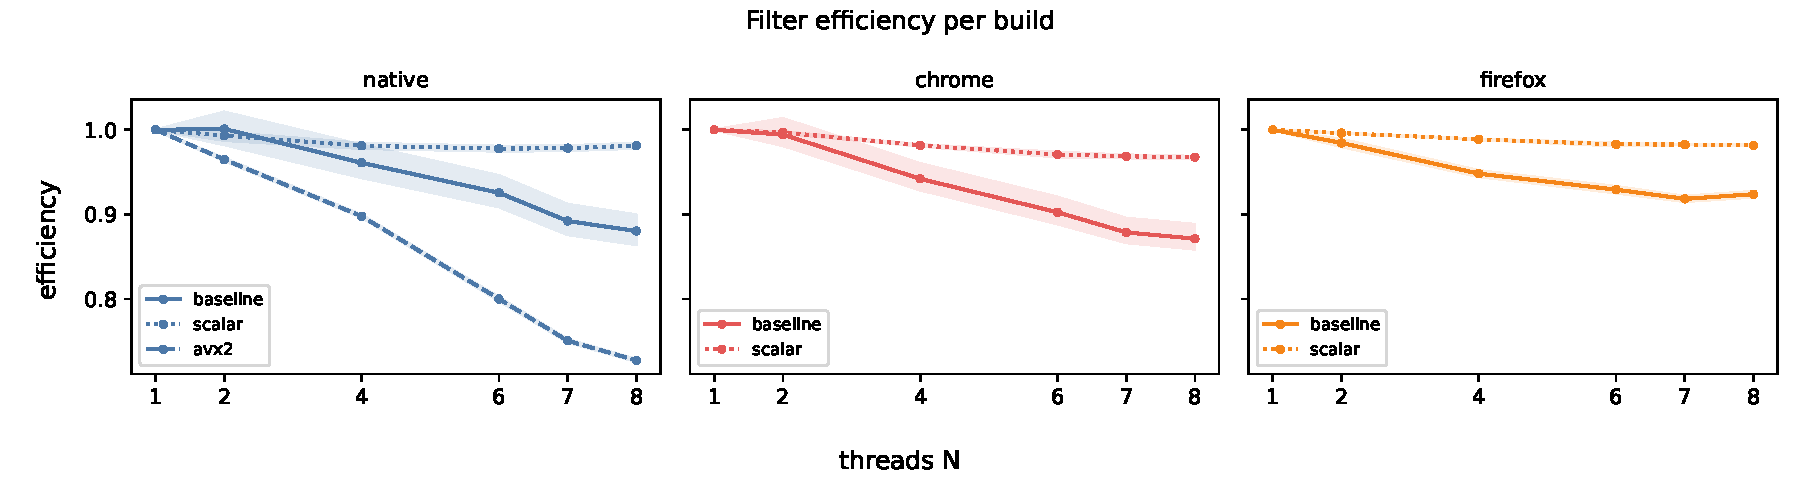
\includegraphics[width=\linewidth]{../figures/simd-efficiency.pdf}
\caption{Filter efficiency per build: scalar (no SIMD on either side), the
baseline (128-bit SIMD) and native AVX2.}
\Description{Efficiency against thread count for the scalar, baseline and AVX2 builds of the filter, one panel per environment.}
\label{fig:simd}
\end{figure}

\emph{The SIMD builds} (720 runs; Table~\ref{tab:simd},
Figure~\ref{fig:simd}). Two builds of the filter change only vectorization:
\emph{scalar}, with the vectorizers off natively and no \code{simd128} in
WASM, and native \emph{AVX2}. Ordered by what one thread reads per second,
the efficiency at eight threads falls on one curve across three builds and
three environments: 0.98, 0.97 and 0.98 for the scalar builds at 476 to
760~MB/s; 0.92 (Firefox), 0.87 (Chrome) and 0.87 (native) for the baseline
at 2178, 2533 and 2969~MB/s; 0.72 for AVX2 at 4337~MB/s. The faster one
thread goes through memory, the less eight threads gain, and Firefox's
baseline filter sits where its throughput puts it. At eight threads the
native baseline filter reads 20.6~GB/s and writes as much.

\emph{The image size.} Natively the efficiency at eight threads is 0.940 at
4096$^2$, where input and output together are 32~MB and fit the last-level
cache, and 0.866 at 8192$^2$, where they are 128~MB
(Table~\ref{tab:cutoff}). The browsers do not show this cleanly (Chrome
0.758 and 0.863, Firefox 0.885 and 0.928): the size supports the reading
natively and is not clear for the browsers.

\emph{An intervention inside one engine.} With the slower baseline compiler
the filter scales slightly better in both browsers (speedup at eight
threads: Chrome 7.09 against 6.83 with the optimizing compiler, Firefox
7.51 against 7.44, Table~\ref{tab:tier}).

So Firefox does not scale better because of how it runs threads. Its filter
does more work between two accesses to memory, and eight such threads ask
less of the memory. In time Firefox stays the slowest at every thread
count. Chrome is the case this does not close: its cycles rise less than
the native ones (1.049) and its efficiency is the native one, so by the
same accounting Chrome loses more outside the loop, which fits the larger
cost of its parallel region and was not measured.

\subsection{The speedup above 8 in Firefox}
\label{sec:why-superlinear}

Firefox's local histogram reaches 8.26 at $k=16$ and 8.48 at $k=256$ with
eight threads. In Firefox a pixel costs fewer cycles with eight threads
than with one: 0.983 times [0.972, 0.994] at $k=16$ and 0.947 [0.881,
0.991] at $k=256$, 5\% fewer, which is the size of the excess over 8. Its
L2 misses per pixel fall by a quarter (0.72 and 0.74 times), those of
native code and Chrome by about a twentieth (0.93 to 0.96). The prediction
held: the one-thread run pays for cache misses that the eight-thread run
does not (question 5, supported). The speedup above 8 is also there against
the sequential reference, so it is not a slow pool. What SpiderMonkey's
one-thread loop does to miss more is not known. This is also what puts
Firefox's RQ2 ratio under 1 at $k=16$ and 256 (question 8).

\subsection{The dip at six and seven threads}
\label{sec:dip}

The local histogram's efficiency dips at $N=6$ and 7 and recovers at 8, in
every environment (natively at $k=16$: 0.956, 0.952, 0.983). The hypothesis
was that Rayon splits work in powers of two, so six or seven threads share
eight pieces unevenly. A campaign of 1080 runs ran the local histogram at
$k=16$ with the adaptive split and with two fixed grains
(Table~\ref{tab:grain-threads}).

\begin{table}[htbp]
\caption{Grain by threads: the local histogram at $k=16$ with Rayon's adaptive split and two fixed grains. Time in ms and efficiency against the one-thread run of the same grain.}\label{tab:grain-threads}
\centering\small
\begin{tabular}{llrrrrrrr}
\toprule
Environment & Grain & $T_1$ & $T_6$ & $E_6$ & $T_7$ & $E_7$ & $T_8$ & $E_8$ \\
\midrule
Native & adaptive & 28.653 & 4.978 & 0.9594 & 4.299 & 0.9521 & 3.630 & 0.9868 \\
Native & 256 KB & 29.810 & 4.985 & 0.9967 & 4.342 & 0.9809 & 3.680 & 1.013 \\
Native & 1024 KB & 29.775 & 5.088 & 0.9754 & 4.589 & 0.9268 & 3.704 & 1.005 \\
\midrule
Chrome & adaptive & 35.729 & 6.322 & 0.9419 & 5.402 & 0.9449 & 4.483 & 0.9963 \\
Chrome & 256 KB & 35.927 & 6.375 & 0.9392 & 5.463 & 0.9395 & 4.748 & 0.9459 \\
Chrome & 1024 KB & 35.738 & 6.520 & 0.9135 & 5.829 & 0.8758 & 4.752 & 0.9402 \\
\midrule
Firefox & adaptive & 36.454 & 6.276 & 0.9681 & 5.401 & 0.9642 & 4.420 & 1.031 \\
Firefox & 256 KB & 36.530 & 6.360 & 0.9573 & 5.489 & 0.9507 & 4.503 & 1.014 \\
Firefox & 1024 KB & 36.211 & 6.477 & 0.9318 & 5.844 & 0.8851 & 4.632 & 0.9772 \\
\bottomrule
\end{tabular}
\end{table}


A fixed grain does not make six or seven threads faster: natively the
times with 256~KB are those of the adaptive split (4.99 against 4.98~ms at
$N=6$) and with 1024~KB they are worse. The efficiencies with a fixed grain
look better only because the one-thread run with a fixed grain is slower
(29.8 against 28.7~ms), which raises every speedup computed from it. In
Chrome and Firefox the times do not improve either. The hypothesis is not
supported; the dip stays unexplained, and placement of six or seven threads
on eight cores was not tested (question 4).

\subsection{The time levels of the contended cells}
\label{sec:levels}

In the counters campaign the atomic histogram at $k=1$ with eight threads
spreads over 25\% to 32\% between its fastest and slowest run, and a run's
time follows its own count of contended line transfers: Spearman's $\rho$
between the time and the lines taken for writing from another core is
$+0.94$ in Chrome, $+0.63$ natively and $+0.56$ in Firefox; in Chrome it is
also $+0.92$ with the compare-and-swap attempts. At $k=256$ the runs are
within 1\% and there is nothing to follow. The levels are states of
contention that differ from run to run (question 9, supported); what sets
the state of a run is not known. Thread placement, left to the kernel, is a
candidate.

\subsection{What stays open}

Why SpiderMonkey's filter loop runs fewer instructions per cycle than
V8's, and why its local histogram misses more with one thread; what Chrome
loses outside the loop; the mechanism that makes the compare-and-swap
faster at $k=256$; the dip at six and seven threads; what sets a run's
state of contention; the slow early iterations of one Firefox cell; and the
step of the fork-join cost at eight threads.

\section{The Exploratory Campaigns}
\label{sec:exploratory}

Seven groups of campaigns ran on the same build with the same protocol (30
runs per cell, the same machine state, start delay and warm-up rules).
Three of them (the engine arms, the counters, the grain by threads) were
used in Section~\ref{sec:why}. The rest bound the primary results: they say
how far the two answers reach. All are exploratory: 95\% intervals, no
correction, no primary conclusion rests on them.

\subsection{Atomics without sharing, atomics with false sharing, sorts}
\label{sec:extras}

The extras campaign (5400 runs, 16.5 hours) measured a ladder at the two
ends of the contention sweep: local counters, \emph{private} atomics (one
padded table per thread), shared padded atomics, and \emph{packed} shared
atomics (eight counters per line), plus two parallel sorts
(Table~\ref{tab:extras}, Figures~\ref{fig:extras-speedup}
to~\ref{fig:extras-rq2}).

\begin{table}[htbp]
\caption{Extras campaign (5400 runs): time in ms at $N=1$ and 8, speedup at $N=8$ with its 95\,\% interval, and the time at $N=8$ over the native one.}\label{tab:extras}
\centering\scriptsize
\resizebox{\linewidth}{!}{%
\begin{tabular}{lrrcrrcrrrcr}
\toprule
 & \multicolumn{3}{c}{Native} & \multicolumn{4}{c}{Chrome} & \multicolumn{4}{c}{Firefox} \\
Workload & $T_1$ & $T_8$ & $S_8$ & $T_1$ & $T_8$ & $S_8$ & /nat. & $T_1$ & $T_8$ & $S_8$ & /nat. \\
\midrule
atomic, $k$=1 & 379.6 & 878.0 & 0.432 [0.421, 0.444] & 698.0 & 1805.4 & 0.387 [0.374, 0.400] & 2.06 & 379.7 & 891.5 & 0.426 [0.414, 0.439] & 1.02 \\
packed, $k$=1 & 381.2 & 878.8 & 0.434 [0.422, 0.446] & 699.9 & 1871.1 & 0.374 [0.360, 0.389] & 2.13 & 380.1 & 886.0 & 0.429 [0.418, 0.440] & 1.01 \\
private, $k$=1 & 379.6 & 47.674 & 7.963 [7.957, 7.968] & 697.9 & 88.031 & 7.928 [7.923, 7.933] & 1.85 & 379.7 & 47.800 & 7.944 [7.937, 7.950] & 1.00 \\
local, $k$=1 & 154.9 & 19.475 & 7.955 [7.952, 7.958] & 150.7 & 19.008 & 7.927 [7.917, 7.937] & 0.98 & 155.6 & 19.775 & 7.871 [7.861, 7.879] & 1.02 \\
\midrule
atomic, $k$=256 & 379.6 & 414.6 & 0.915 [0.914, 0.917] & 411.9 & 210.3 & 1.959 [1.958, 1.960] & 0.51 & 379.8 & 392.8 & 0.967 [0.966, 0.968] & 0.95 \\
packed, $k$=256 & 379.8 & 490.3 & 0.775 [0.772, 0.777] & 407.7 & 725.7 & 0.562 [0.560, 0.563] & 1.48 & 379.8 & 492.0 & 0.772 [0.769, 0.775] & 1.00 \\
private, $k$=256 & 379.6 & 47.677 & 7.961 [7.952, 7.970] & 411.6 & 52.110 & 7.900 [7.892, 7.907] & 1.09 & 379.9 & 47.835 & 7.941 [7.934, 7.948] & 1.00 \\
local, $k$=256 & 27.104 & 3.422 & 7.921 [7.898, 7.943] & 33.391 & 4.195 & 7.960 [7.861, 8.068] & 1.23 & 34.528 & 4.139 & 8.341 [8.189, 8.530] & 1.21 \\
\midrule
sort & 1468.0 & 188.5 & 7.789 [7.786, 7.793] & 1600.0 & 205.8 & 7.775 [7.773, 7.778] & 1.09 & 1531.7 & 196.3 & 7.802 [7.799, 7.804] & 1.04 \\
sort-unstable & 539.2 & 84.358 & 6.392 [6.389, 6.396] & 683.6 & 109.9 & 6.221 [6.217, 6.224] & 1.30 & 682.1 & 110.2 & 6.187 [6.182, 6.191] & 1.31 \\
\bottomrule
\end{tabular}
}
\end{table}


\begin{figure}[tbp]
\centering
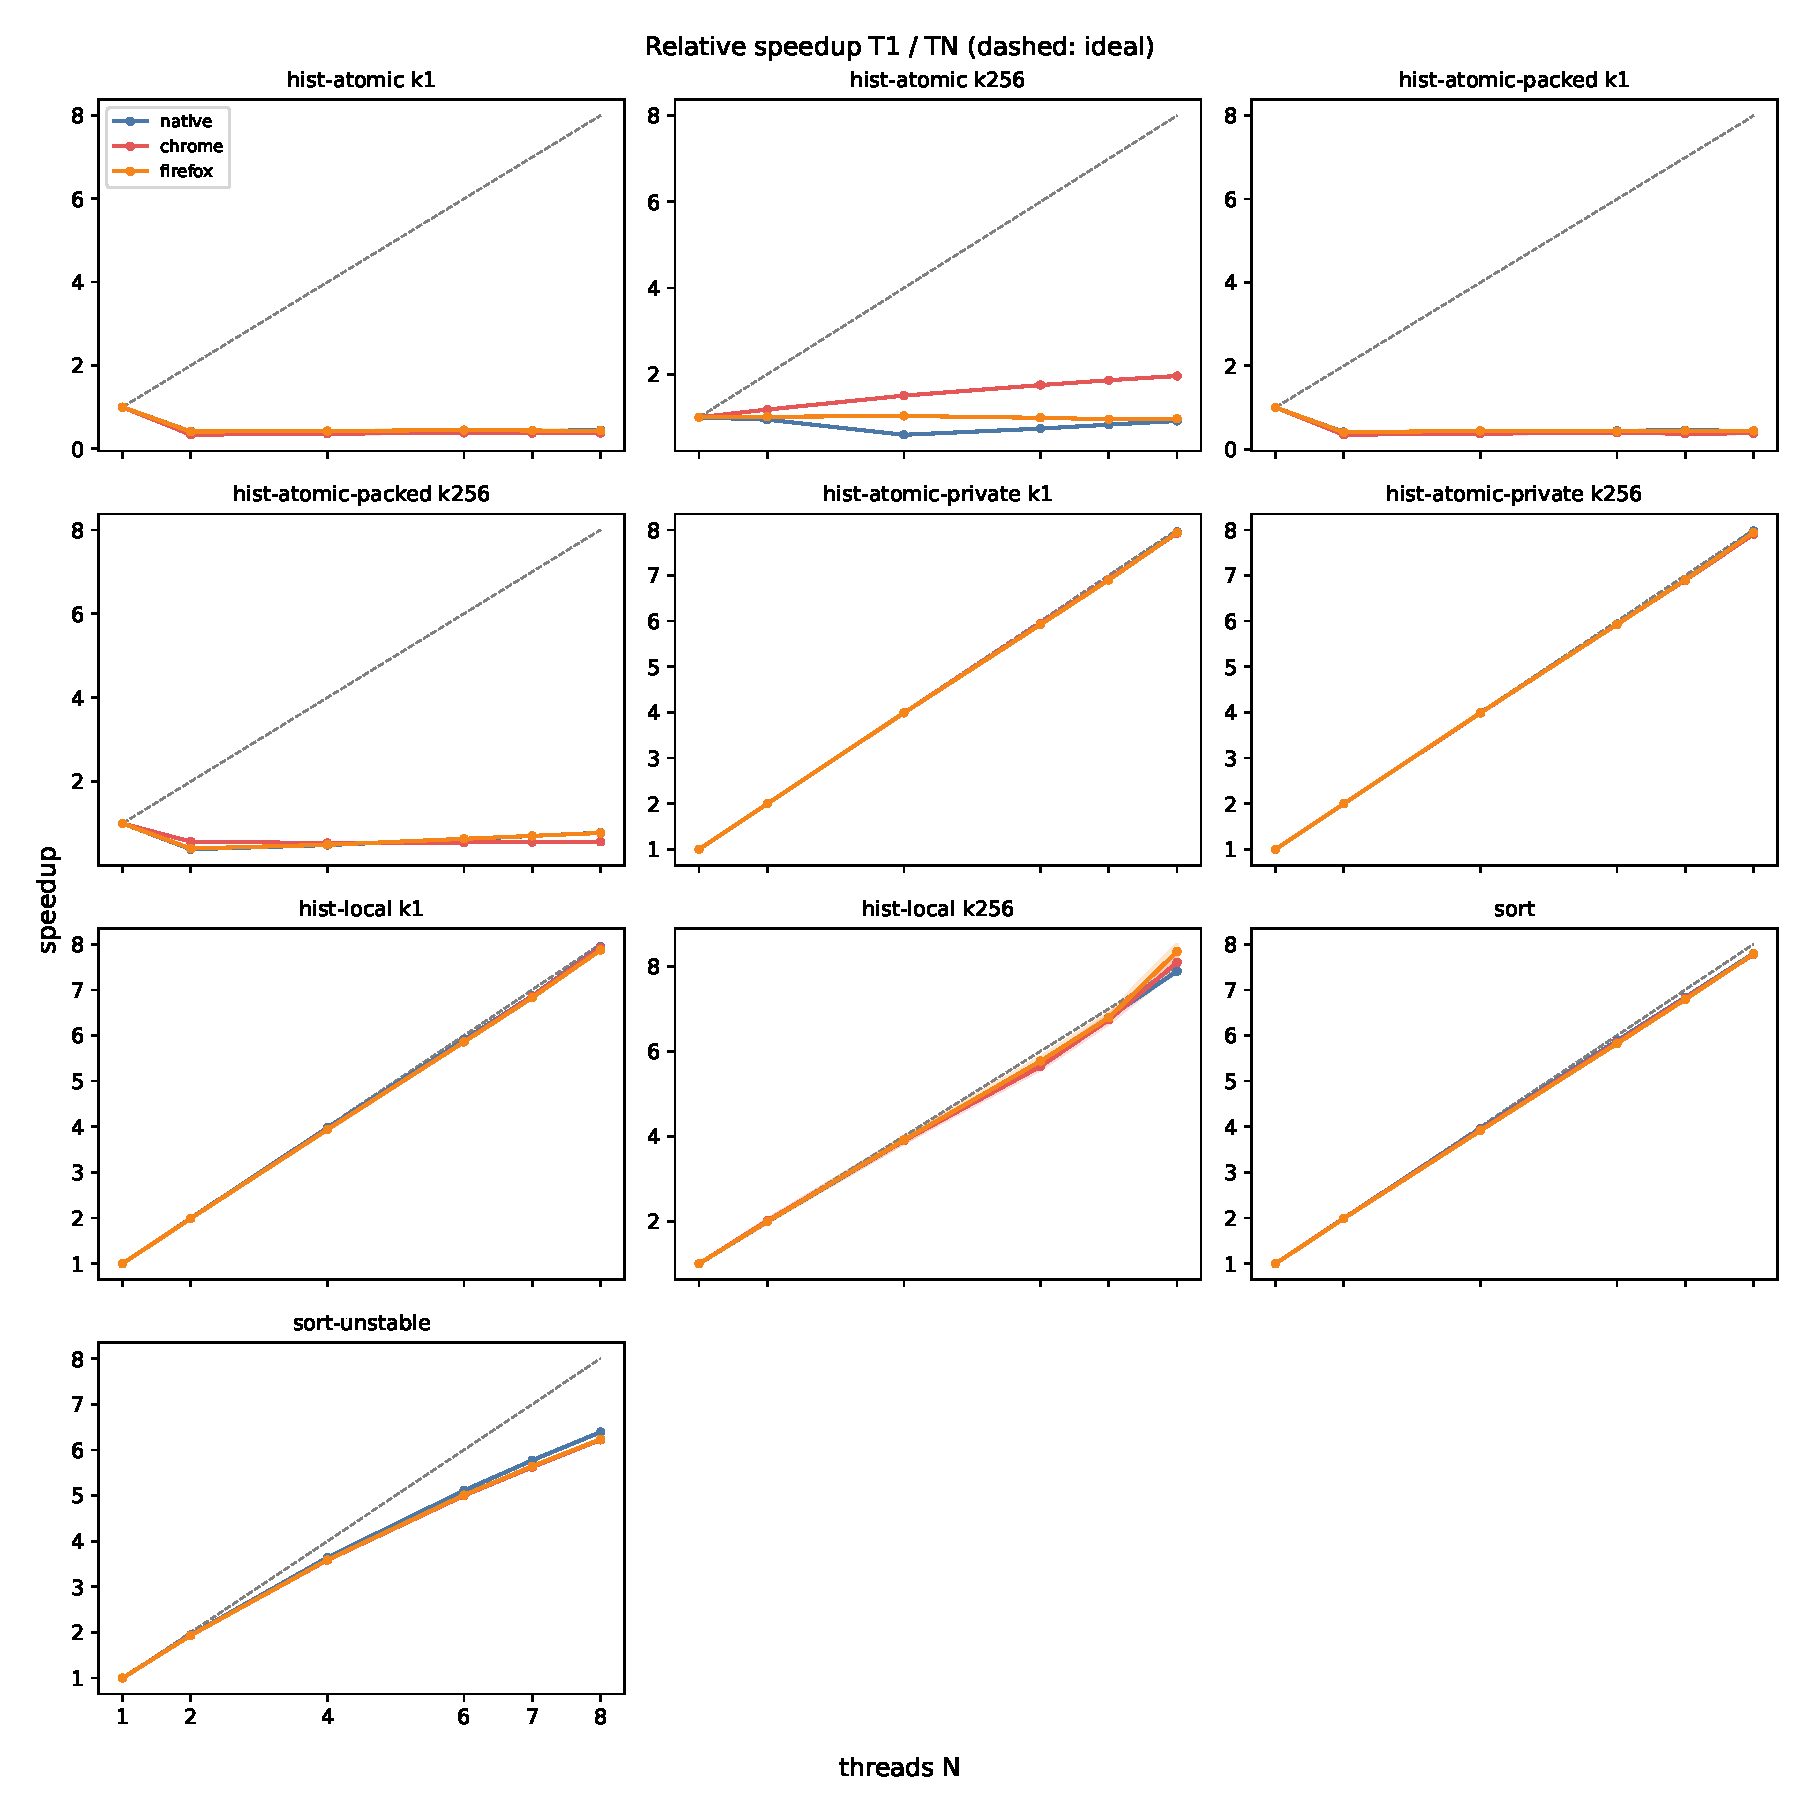
\includegraphics[width=0.8\linewidth]{../figures/extras-speedup.pdf}
\caption{Extras campaign: relative speedup per workload.}
\Description{Speedup against thread count for the extras workloads in the three environments.}
\label{fig:extras-speedup}
\end{figure}

\begin{figure}[tbp]
\centering
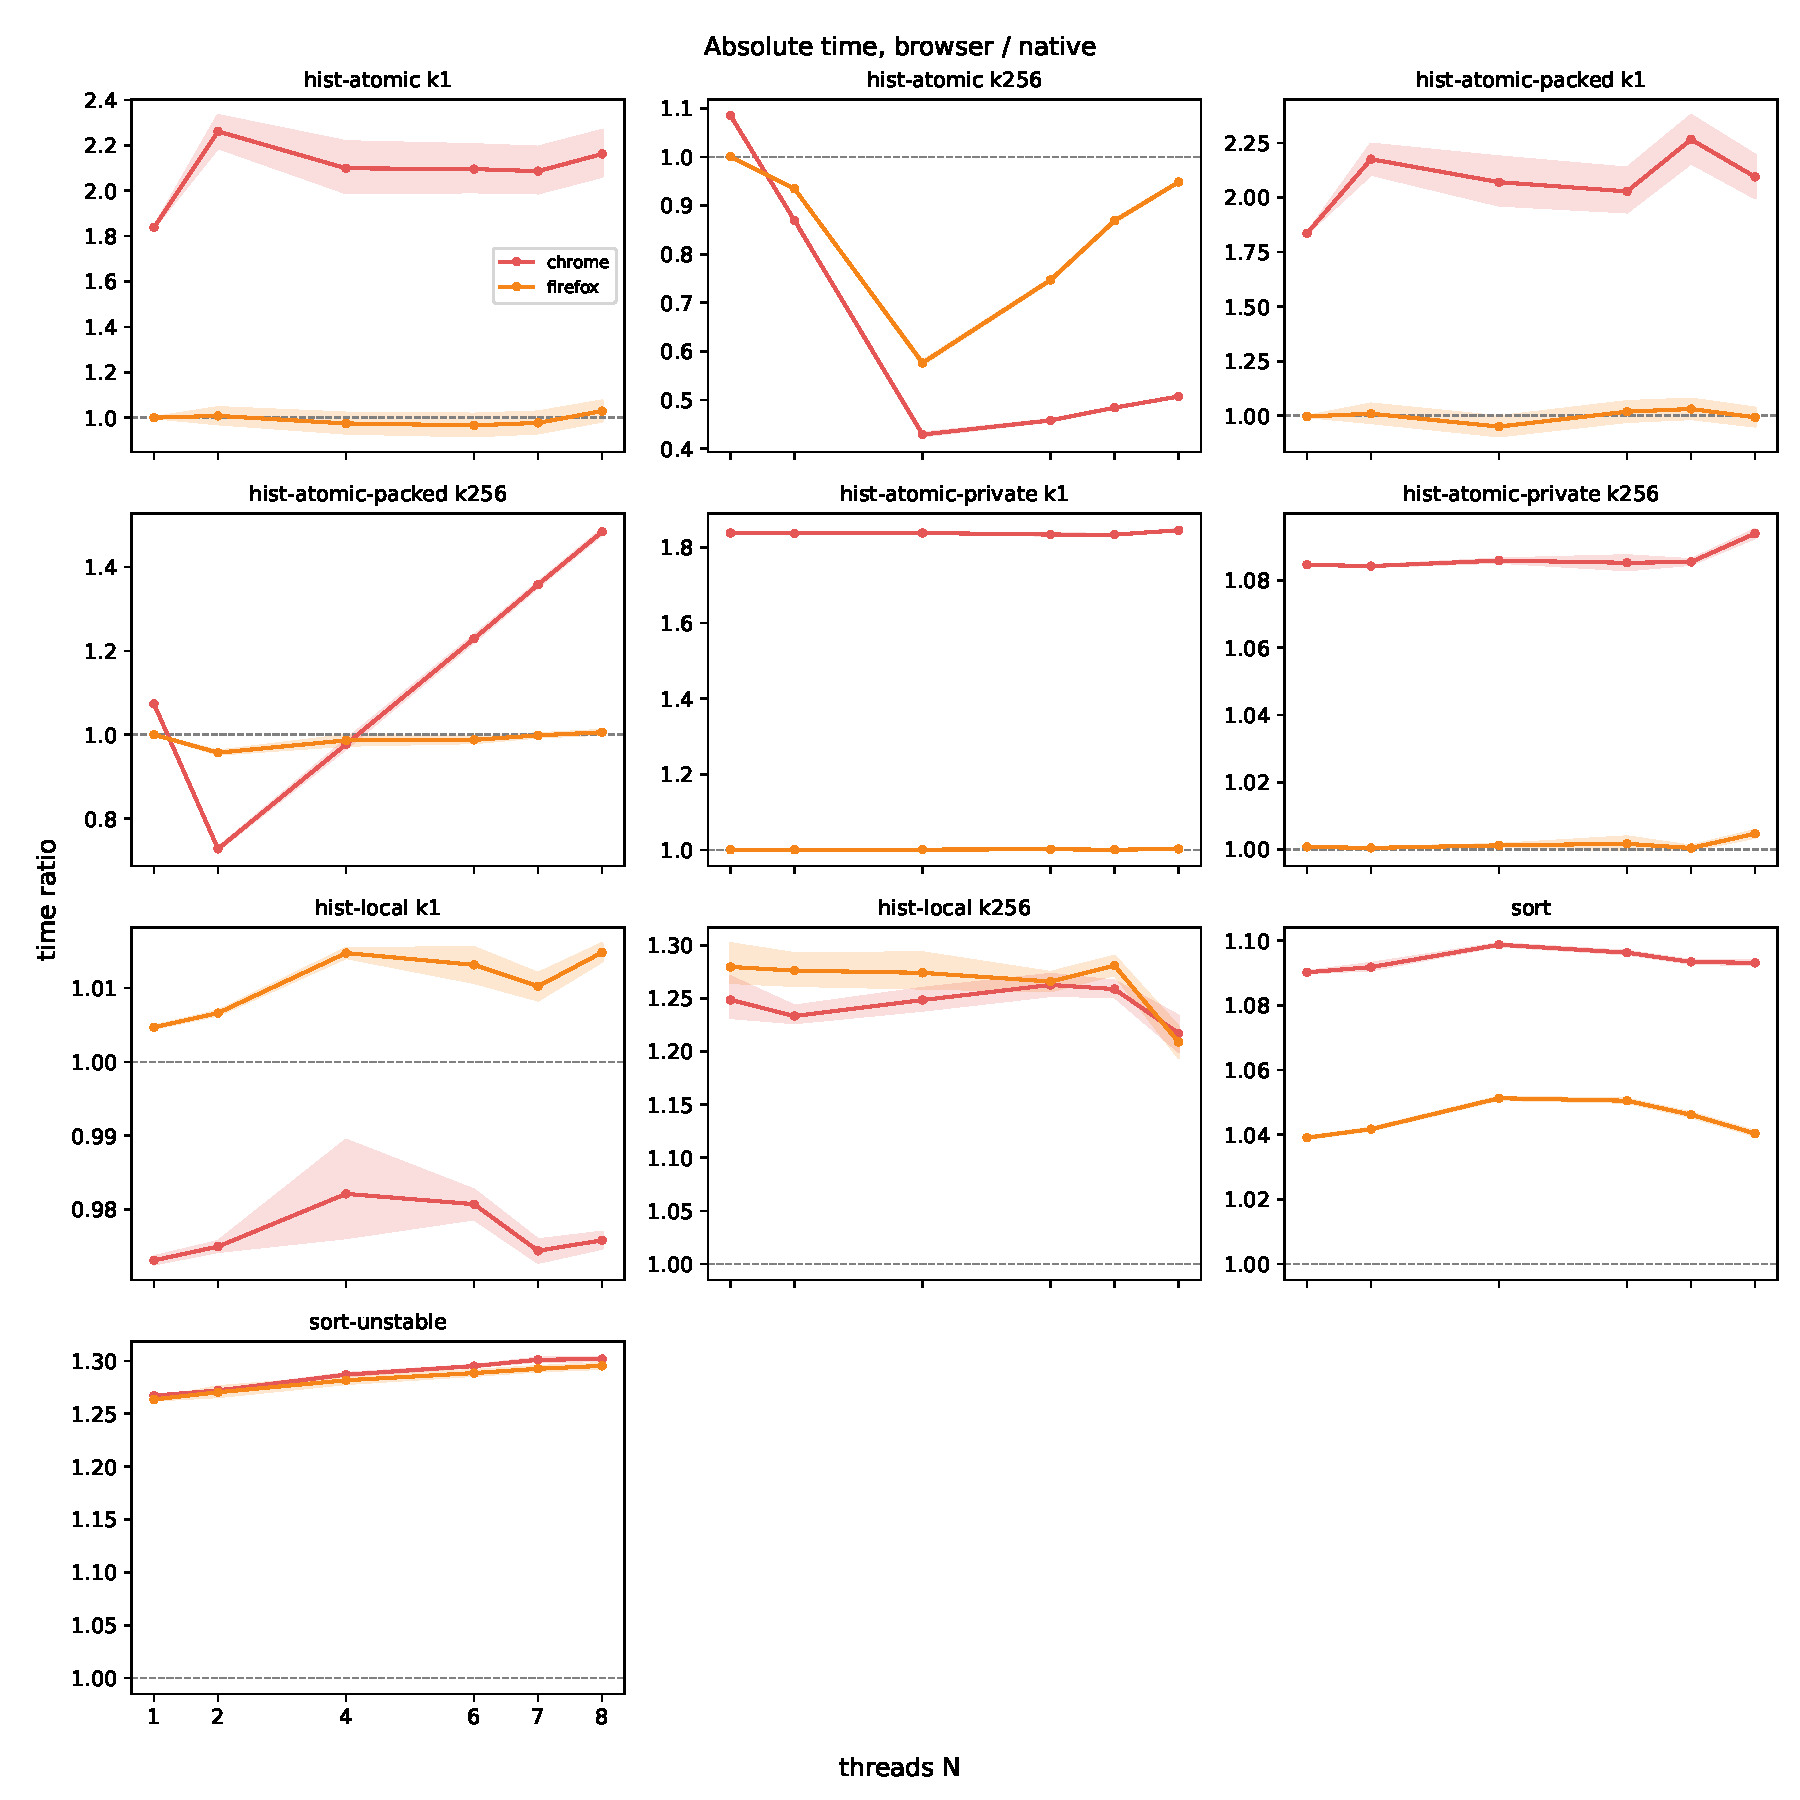
\includegraphics[width=0.8\linewidth]{../figures/extras-absolute.pdf}
\caption{Extras campaign: absolute time per workload and environment.}
\Description{Absolute time against thread count for the extras workloads.}
\label{fig:extras-absolute}
\end{figure}

\begin{figure}[tbp]
\centering
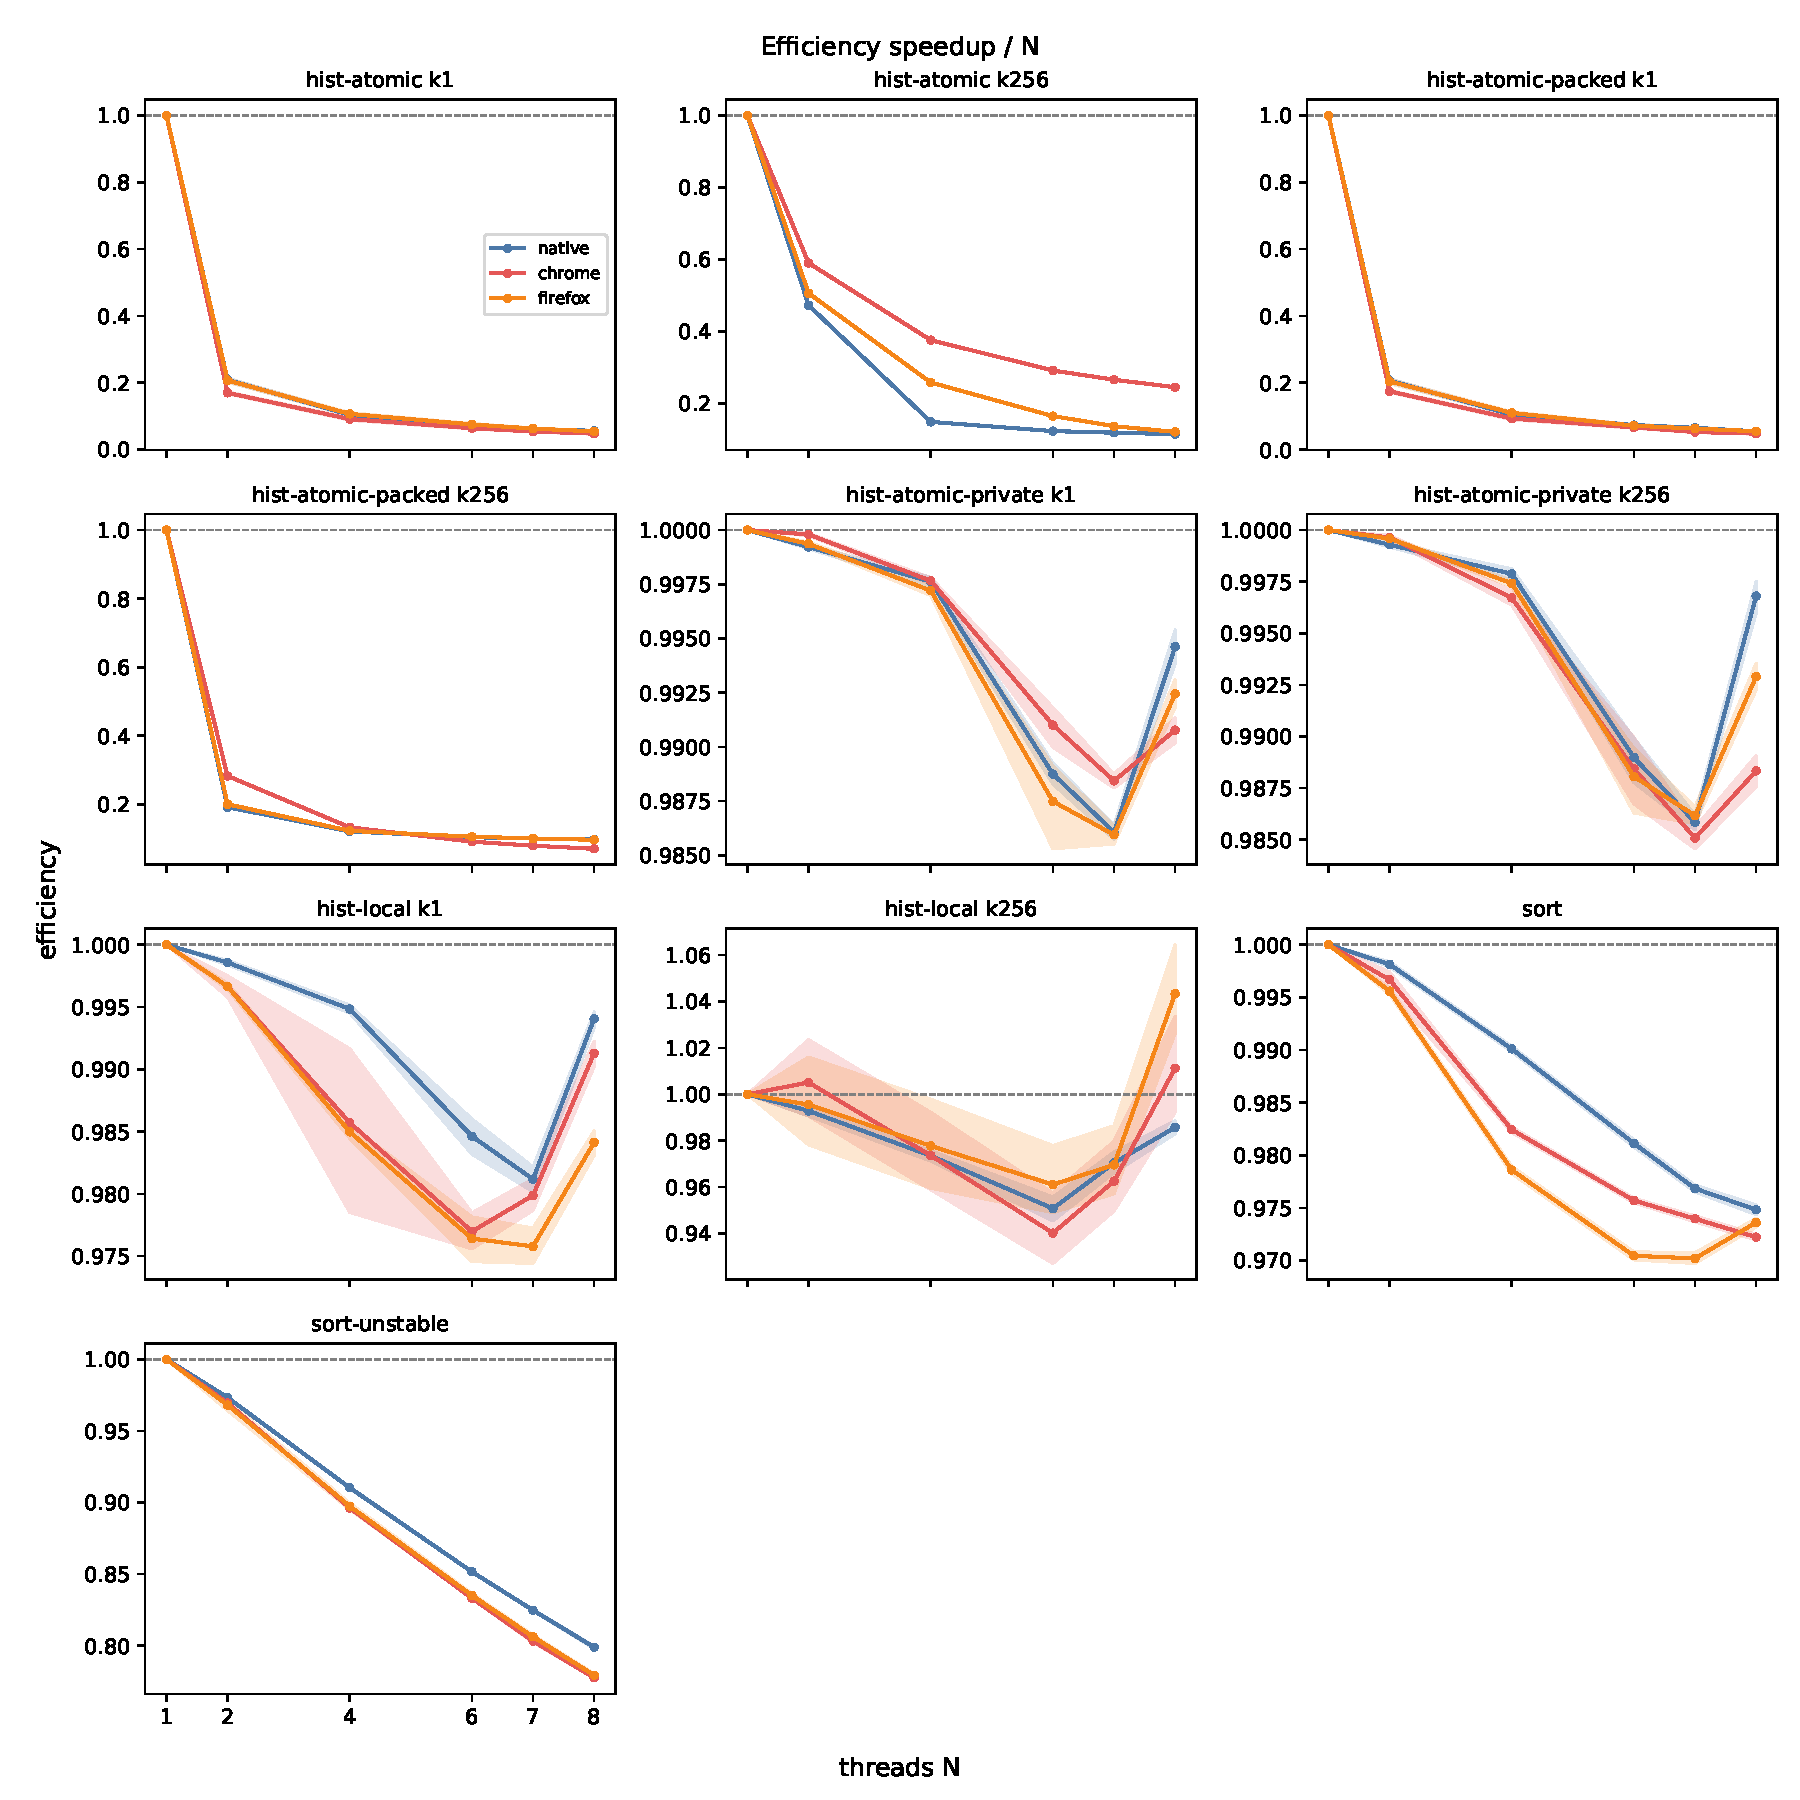
\includegraphics[width=0.8\linewidth]{../figures/extras-efficiency.pdf}
\caption{Extras campaign: efficiency per workload.}
\Description{Efficiency against thread count for the extras workloads.}
\label{fig:extras-efficiency}
\end{figure}

\begin{figure}[tbp]
\centering
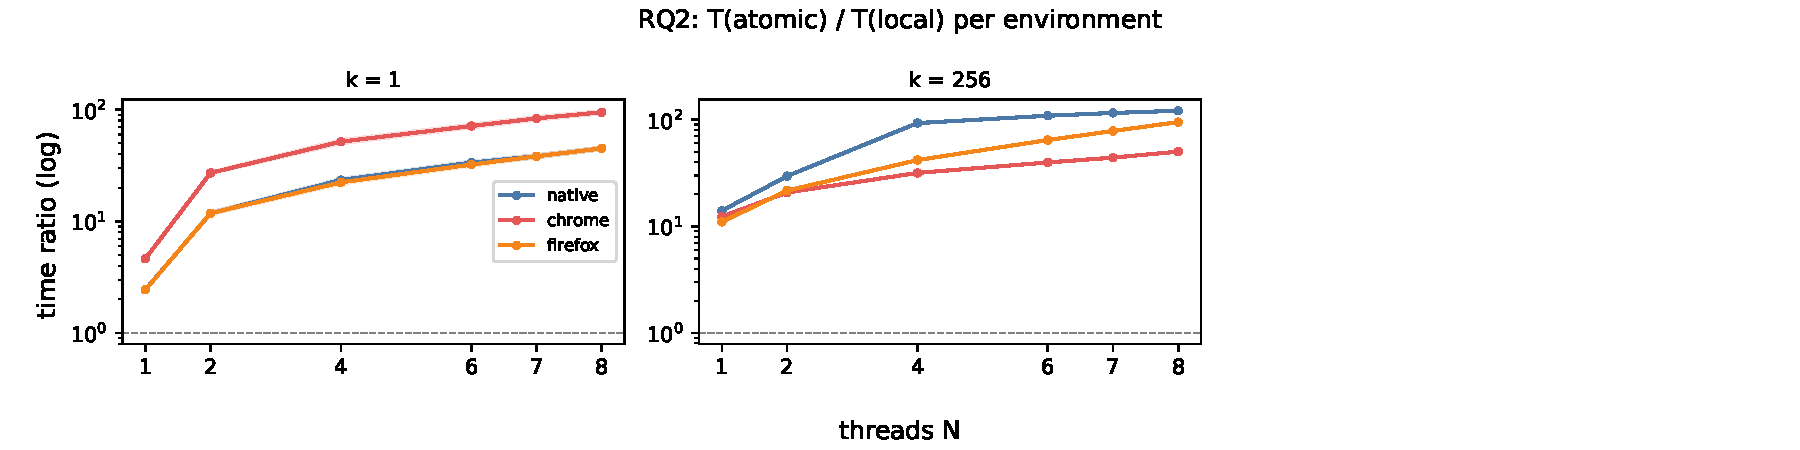
\includegraphics[width=\linewidth]{../figures/extras-rq2.pdf}
\caption{Extras campaign: $T_{\mathrm{atomic}}/T_{\mathrm{local}}$ against
$N$ for the shared padded atomics at $k=1$ and 256, measured again.}
\Description{Atomic over local time ratio against thread count in the extras campaign.}
\label{fig:extras-rq2}
\end{figure}

\begin{itemize}[leftmargin=1.5em]
\item \emph{The cells shared with the main campaign reproduce it.} The
local and shared histograms at $k=1$ and 256 were measured again,
interleaved, in this campaign: for example the shared atomics at $k=256$,
$N=8$ take 414.6, 210.3 and 392.8~ms here against 414.6, 210.4 and 393.0 in
the main campaign.
\item \emph{Private atomics scale like the local control} (speedup 7.90 to
7.96 in the three environments): the atomic instruction alone does not hurt
scaling. But it costs Chrome 88.0~ms at $k=1$, $N=8$ against 47.7~ms
natively and 47.8 in Firefox (1.85 times), and 52.1 against 47.7~ms at
$k=256$ (1.09 times). No line is shared here, so this is the cost of V8's
sequence without contention; it has the shape the native probe found for
the compare-and-swap with one thread (slower at $k=1$, close to the locked
add at $k=256$). Firefox matches native. Shared against private then gives
the part that contention adds: at $k=1$ Chrome's shared histogram takes
2.06 times the native one where its private one takes 1.85 times.
\item \emph{Packing the counters removes Chrome's advantage.} With eight
counters per line the atomic histogram at $k=256$, $N=8$ slows by 1.18
times natively (490 against 415~ms), 1.25 times in Firefox and 3.45 times
in Chrome (726 against 210~ms), which then takes 1.48 times the native
time. Chrome's advantage under spread contention depends on each counter
having its own line. At $k=1$ packing changes little (within 4\%): one counter is hit.
\item \emph{Sorts.} The stable parallel sort, which allocates, reaches
7.78 to 7.80 at $N=8$ in the three environments at 1.04 (Firefox) and 1.09
(Chrome) times the native time; the unstable in-place sort reaches 6.19 to
6.39 at 1.30 and 1.31 times. The sort that goes through WASM's allocator
does not show the larger gap, so the allocator's global lock is not visible
at this allocation rate.
\end{itemize}
One configuration trends with the execution order (Chrome, private, $k=1$,
$N=2$). Against the earlier build, every cell at eight threads is within
1\% of its v2 time except the two shared counters at $k=1$ (within 3.4\%),
the cells whose runs fall on levels; this is a consistency observation, not
a comparison of results.

\clearpage
\subsection{Weak scaling}

In strong scaling each thread gets $1/N$ of the work; in weak scaling the
input grows with $N$. The campaign (1080 runs) used an image 8192 pixels
wide and $1024N$ rows high, so that every thread gets the work it has in
the main campaign at $N=8$ (Table~\ref{tab:weak},
Figure~\ref{fig:weak}).

\begin{table}[htbp]
\caption{Weak scaling (1080 runs): the image is 8192 pixels wide and $1024N$ rows high. Time in ms and weak efficiency $T_1/T_N$ with its 95\,\% interval.}\label{tab:weak}
\centering\footnotesize
\begin{tabular}{llrcrcrc}
\toprule
 &  & \multicolumn{2}{c}{Native} & \multicolumn{2}{c}{Chrome} & \multicolumn{2}{c}{Firefox} \\
Workload & $N$ & $T_N$ & $T_1/T_N$ & $T_N$ & $T_1/T_N$ & $T_N$ & $T_1/T_N$ \\
\midrule
filter & 1 & 2.804 & 1.000 [1.000, 1.000] & 3.269 & 1.000 [1.000, 1.000] & 3.817 & 1.000 [1.000, 1.000] \\
filter & 2 & 3.007 & 0.932 [0.930, 0.935] & 3.492 & 0.936 [0.932, 0.941] & 4.011 & 0.951 [0.943, 0.960] \\
filter & 4 & 3.130 & 0.896 [0.893, 0.898] & 3.713 & 0.880 [0.875, 0.886] & 4.196 & 0.910 [0.902, 0.917] \\
filter & 6 & 3.164 & 0.886 [0.884, 0.888] & 3.807 & 0.859 [0.854, 0.863] & 4.222 & 0.904 [0.898, 0.910] \\
filter & 7 & 3.231 & 0.868 [0.866, 0.869] & 3.866 & 0.845 [0.841, 0.850] & 4.226 & 0.903 [0.898, 0.908] \\
filter & 8 & 3.259 & 0.860 [0.858, 0.863] & 3.843 & 0.851 [0.847, 0.855] & 4.172 & 0.915 [0.908, 0.922] \\
\midrule
local, $k$=1 & 1 & 19.427 & 1.000 [1.000, 1.000] & 18.867 & 1.000 [1.000, 1.000] & 19.672 & 1.000 [1.000, 1.000] \\
local, $k$=1 & 2 & 19.451 & 0.999 [0.998, 0.999] & 18.928 & 0.997 [0.995, 0.998] & 19.772 & 0.995 [0.994, 0.996] \\
local, $k$=1 & 4 & 19.519 & 0.995 [0.994, 0.996] & 18.996 & 0.993 [0.992, 0.994] & 19.803 & 0.993 [0.992, 0.994] \\
local, $k$=1 & 6 & 19.800 & 0.981 [0.979, 0.983] & 19.223 & 0.981 [0.978, 0.985] & 20.010 & 0.983 [0.981, 0.985] \\
local, $k$=1 & 7 & 19.718 & 0.985 [0.982, 0.988] & 19.216 & 0.982 [0.979, 0.985] & 19.947 & 0.986 [0.985, 0.988] \\
local, $k$=1 & 8 & 19.488 & 0.997 [0.996, 0.998] & 19.007 & 0.993 [0.992, 0.994] & 19.790 & 0.994 [0.993, 0.995] \\
\bottomrule
\end{tabular}
\end{table}


\begin{figure}[tbp]
\centering
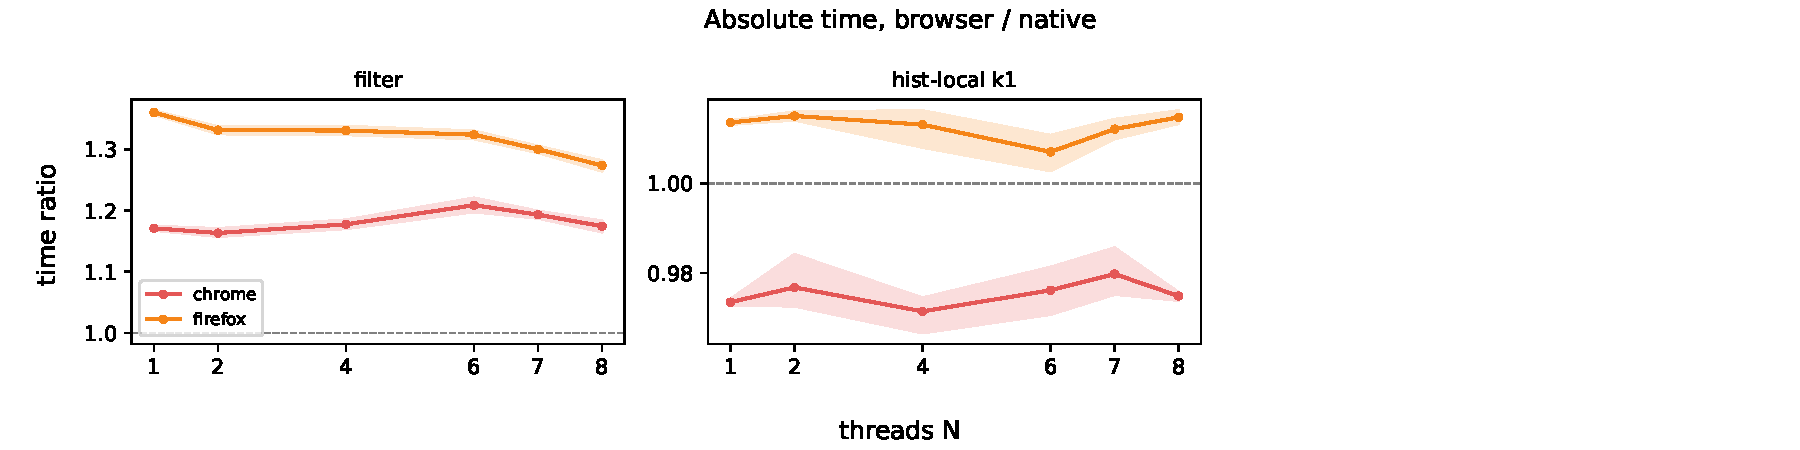
\includegraphics[width=0.75\linewidth]{../figures/weak-absolute.pdf}
\caption{Weak scaling: absolute time against $N$ (ideal: flat).}
\Description{Absolute time against thread count in weak scaling for the filter and the local histogram.}
\label{fig:weak}
\end{figure}

At eight threads the filter keeps 0.860 of its one-thread rate natively
[0.858, 0.863], 0.851 in Chrome and 0.915 in Firefox; the local histogram
0.993 to 0.997. These are the strong-scaling efficiencies (0.869, 0.865,
0.917) within one to two points: the filter's loss is the same whether the
work per thread shrinks or stays fixed, which fits a cost of sharing the
memory and not a serial part. The browser over native time ratio stays flat
in Chrome (1.16 to 1.20) and falls in Firefox from 1.36 at $N=1$ to 1.28 at
$N=8$.

\clearpage
\subsection{E-cores}

The hybrid campaign (900 runs) put the eight P-cores and twelve E-cores in
the mask and ran $N$ up to 20, to see how work stealing copes with cores of
two speeds (Table~\ref{tab:hybrid}, Figures~\ref{fig:hybrid-speedup}
and~\ref{fig:hybrid-absolute}).

\begin{table}[htbp]
\caption{Hybrid campaign (900 runs): 8 P-cores and 12 E-cores in the mask. Time in ms and speedup $T_1/T_N$ with its 95\,\% interval.}\label{tab:hybrid}
\centering\footnotesize
\begin{tabular}{llrcrcrc}
\toprule
 &  & \multicolumn{2}{c}{Native} & \multicolumn{2}{c}{Chrome} & \multicolumn{2}{c}{Firefox} \\
Workload & $N$ & $T_N$ & $S_N$ & $T_N$ & $S_N$ & $T_N$ & $S_N$ \\
\midrule
filter & 1 & 22.628 & 1.000 [1.000, 1.000] & 26.487 & 1.000 [1.000, 1.000] & 30.774 & 1.000 [1.000, 1.000] \\
filter & 8 & 3.503 & 6.460 [6.330, 6.569] & 4.046 & 6.547 [6.487, 6.601] & 4.385 & 7.018 [6.934, 7.096] \\
filter & 12 & 3.028 & 7.472 [7.303, 7.627] & 3.484 & 7.603 [7.544, 7.660] & 3.739 & 8.231 [8.135, 8.326] \\
filter & 16 & 2.879 & 7.861 [7.815, 7.904] & 3.463 & 7.648 [7.591, 7.706] & 3.551 & 8.666 [8.604, 8.726] \\
filter & 20 & 2.827 & 8.005 [7.978, 8.032] & 3.475 & 7.622 [7.584, 7.659] & 3.569 & 8.622 [8.556, 8.687] \\
\midrule
local, $k$=1 & 1 & 154.9 & 1.000 [1.000, 1.000] & 150.7 & 1.000 [1.000, 1.000] & 155.7 & 1.000 [1.000, 1.000] \\
local, $k$=1 & 8 & 19.631 & 7.893 [7.860, 7.935] & 18.655 & 8.078 [7.907, 8.280] & 19.830 & 7.850 [7.808, 7.907] \\
local, $k$=1 & 12 & 11.568 & 13.394 [13.209, 13.609] & 8.893 & 16.946 [16.578, 17.364] & 10.320 & 15.084 [14.805, 15.366] \\
local, $k$=1 & 16 & 7.973 & 19.433 [19.195, 19.683] & 5.979 & 25.207 [24.908, 25.509] & 7.432 & 20.945 [20.476, 21.421] \\
local, $k$=1 & 20 & 6.078 & 25.495 [25.046, 25.915] & 5.112 & 29.480 [28.850, 30.092] & 6.140 & 25.353 [25.039, 25.688] \\
\bottomrule
\end{tabular}
\end{table}


\begin{figure}[tbp]
\centering
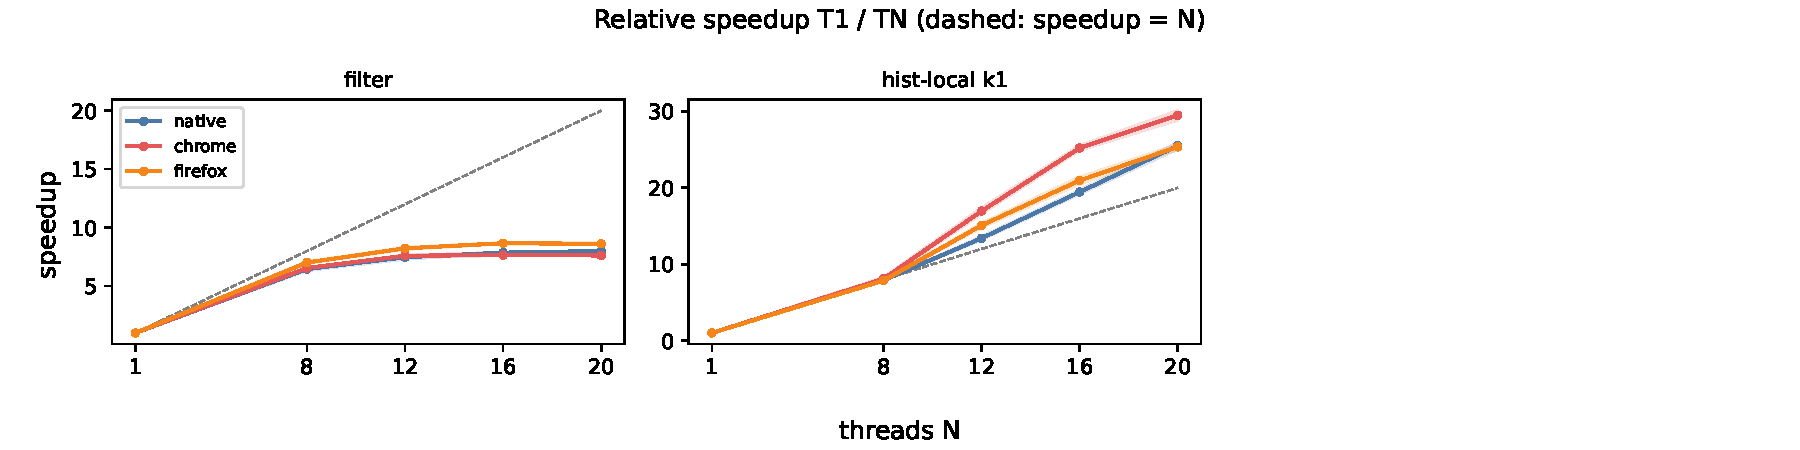
\includegraphics[width=0.75\linewidth]{../figures/hybrid-speedup.pdf}
\caption{Hybrid campaign: speedup against $N$ with P-cores and E-cores.}
\Description{Speedup against thread count up to twenty threads for the filter and the local histogram.}
\label{fig:hybrid-speedup}
\end{figure}

\begin{figure}[tbp]
\centering
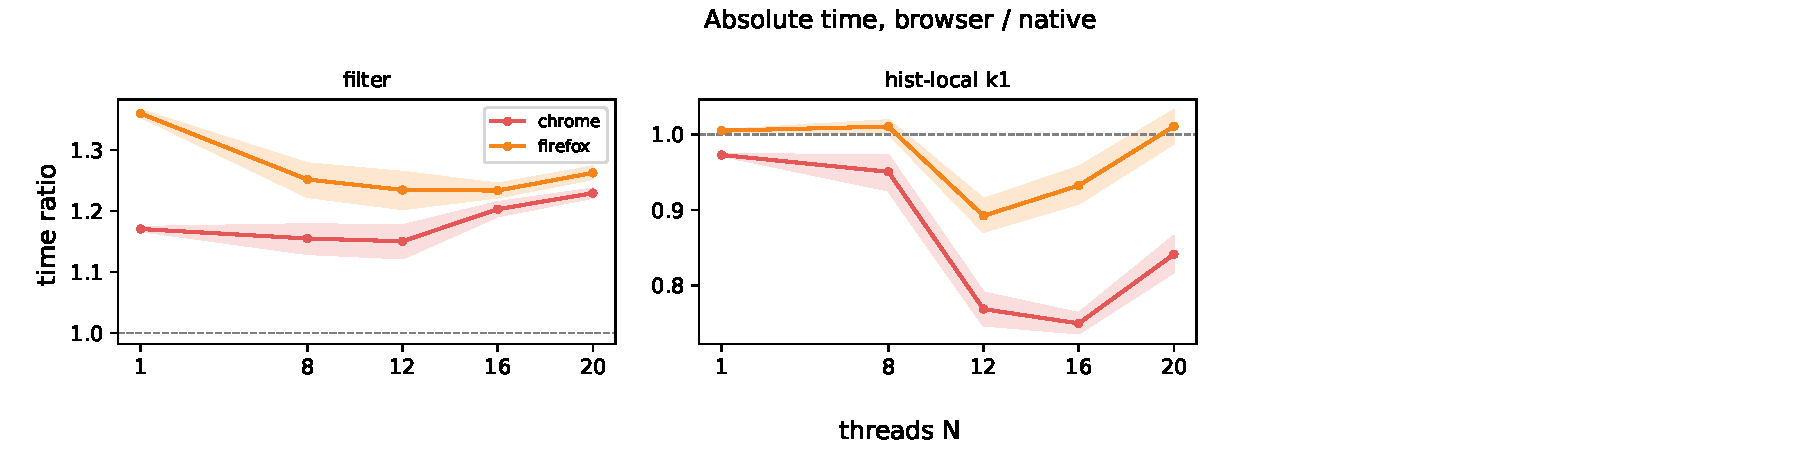
\includegraphics[width=0.75\linewidth]{../figures/hybrid-absolute.pdf}
\caption{Hybrid campaign: absolute time against $N$.}
\Description{Absolute time against thread count up to twenty threads.}
\label{fig:hybrid-absolute}
\end{figure}

The filter gains little from the E-cores: its speedup goes from 6.46 at
eight threads to 8.01 at twenty natively, 6.55 to 7.62 in Chrome and 7.02
to 8.62 in Firefox; in Chrome it is flat from twelve threads on. The three
environments use the extra cores about alike. The local histogram at $k=1$
goes far beyond the thread count (25.5 natively, 29.5 in Chrome and 25.4 in
Firefox at twenty threads): its one-thread time is a dependent chain on a
P-core, and the analysis of the earlier build traced the excess to the
E-cores running that chain faster than the P-cores do. Which threads the
kernel puts on which kind of core is not controlled and not recorded per
thread, and the cells with E-cores vary more than the others. With the
wider mask the eight-thread cells are slower than in the P-only campaign
(native filter 3.50 against 3.25~ms), as the mask pilot had found.

\clearpage
\subsection{Small regions: the cutoff}
\label{sec:cutoff}

RQ1 is answered at one size, where the work of a parallel region dominates
its fixed cost. The cutoff campaigns ask where that stops: five image sides
from 512 to 8192, $N \in \{1,2,4,8\}$, the filter and the local histogram
at $k=256$ (3600 runs, plus 480 native control runs). A 512$^2$ filter on
eight threads takes about 26~\textmu s natively, far under the 2~ms that
100 ticks of Firefox's clock need, so each timed sample repeats the work
$K = (8192/\mathrm{side})^2$ times and reports the time per pass. Sizes are
compared only through speedups within a size, where $K$ cancels
(Table~\ref{tab:cutoff}, Figure~\ref{fig:cutoff}).

\begin{figure}[tbp]
\centering
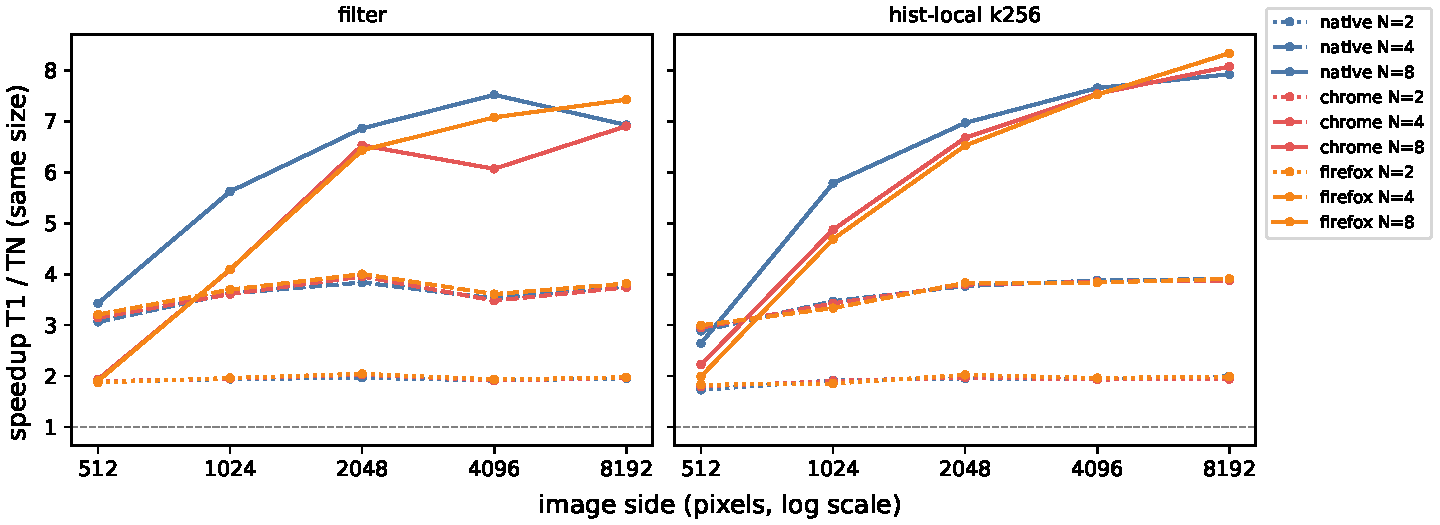
\includegraphics[width=\linewidth]{../figures/cutoff-speedup.pdf}
\caption{Cutoff campaigns: speedup against the image side, per environment
and $N$.}
\Description{Speedup against image side from 512 to 8192 for the filter and the local histogram in the three environments.}
\label{fig:cutoff}
\end{figure}

{\footnotesize
\begin{longtable}{lllccccc}
\caption{Cutoff campaigns: speedup (efficiency) by image side, with repeated passes per timed sample so that small images clear the clock.}\label{tab:cutoff} \\
\toprule
Workload & $N$ & Environment & 512$^2$ & 1024$^2$ & 2048$^2$ & 4096$^2$ & 8192$^2$ \\
\midrule
\endfirsthead
\toprule
Workload & $N$ & Environment & 512$^2$ & 1024$^2$ & 2048$^2$ & 4096$^2$ & 8192$^2$ \\
\midrule
\endhead
\bottomrule
\endfoot
filter & 2 & Native & 1.890 (0.945) & 1.944 (0.972) & 1.968 (0.984) & 1.913 (0.957) & 1.959 (0.979) \\
filter & 2 & Chrome & 1.900 (0.950) & 1.951 (0.975) & 2.029 (1.014) & 1.914 (0.957) & 1.970 (0.985) \\
filter & 2 & Firefox & 1.877 (0.939) & 1.964 (0.982) & 2.047 (1.023) & 1.935 (0.967) & 1.980 (0.990) \\
filter & 4 & Native & 3.063 (0.766) & 3.622 (0.906) & 3.837 (0.959) & 3.523 (0.881) & 3.775 (0.944) \\
filter & 4 & Chrome & 3.145 (0.786) & 3.610 (0.903) & 3.957 (0.989) & 3.481 (0.870) & 3.741 (0.935) \\
filter & 4 & Firefox & 3.207 (0.802) & 3.697 (0.924) & 4.001 (1.000) & 3.610 (0.902) & 3.817 (0.954) \\
filter & 8 & Native & 3.428 (0.429) & 5.622 (0.703) & 6.860 (0.857) & 7.519 (0.940) & 6.926 (0.866) \\
filter & 8 & Chrome & 1.936 (0.242) & 4.086 (0.511) & 6.528 (0.816) & 6.067 (0.758) & 6.905 (0.863) \\
filter & 8 & Firefox & 1.906 (0.238) & 4.095 (0.512) & 6.430 (0.804) & 7.077 (0.885) & 7.424 (0.928) \\
\midrule
local, $k$=256 & 2 & Native & 1.731 (0.866) & 1.918 (0.959) & 1.957 (0.979) & 1.940 (0.970) & 1.995 (0.998) \\
local, $k$=256 & 2 & Chrome & 1.798 (0.899) & 1.907 (0.953) & 1.974 (0.987) & 1.935 (0.967) & 1.943 (0.971) \\
local, $k$=256 & 2 & Firefox & 1.831 (0.916) & 1.855 (0.927) & 2.024 (1.012) & 1.964 (0.982) & 1.991 (0.996) \\
local, $k$=256 & 4 & Native & 2.887 (0.722) & 3.470 (0.868) & 3.768 (0.942) & 3.877 (0.969) & 3.906 (0.977) \\
local, $k$=256 & 4 & Chrome & 2.950 (0.738) & 3.428 (0.857) & 3.796 (0.949) & 3.850 (0.962) & 3.877 (0.969) \\
local, $k$=256 & 4 & Firefox & 2.998 (0.749) & 3.335 (0.834) & 3.830 (0.957) & 3.836 (0.959) & 3.909 (0.977) \\
local, $k$=256 & 8 & Native & 2.644 (0.330) & 5.786 (0.723) & 6.968 (0.871) & 7.651 (0.956) & 7.923 (0.990) \\
local, $k$=256 & 8 & Chrome & 2.227 (0.278) & 4.872 (0.609) & 6.674 (0.834) & 7.538 (0.942) & 8.074 (1.009) \\
local, $k$=256 & 8 & Firefox & 1.995 (0.249) & 4.688 (0.586) & 6.523 (0.815) & 7.523 (0.940) & 8.334 (1.042) \\
\end{longtable}
}

\begin{table}[htbp]
\caption{Cutoff at $N=8$: the image side at which the efficiency crosses 0.5 (interpolated, 95\,\% interval) and the sequential work of that image in \textmu s; then the fork-join model $T_N=W/N+F$ with this campaign's warm fork-join $F$ in \textmu s: the work it predicts for efficiency 0.5, and the side at which $F$ is 1\,\% and 5\,\% of $T_N$.}\label{tab:cutoff-estimates}
\centering\footnotesize
\begin{tabular}{llcrrrrr}
\toprule
Workload & Environment & Side at 0.5 & Work & $F$ & Model & Side 1\,\% & Side 5\,\% \\
\midrule
filter & Native & 613 [610, 616] & 124.9 & 10.8 & 86.1 & 5031 & 2204 \\
local, $k$=256 & Native & 691 [679, 701] & 183.4 & 10.8 & 86.1 & 4595 & 2013 \\
filter & Chrome & 996 [989, 1002] & 395.6 & 105.0 & 840.0 & 14518 & 6360 \\
local, $k$=256 & Chrome & 815 [797, 832] & 324.6 & 105.0 & 840.0 & 12938 & 5668 \\
filter & Firefox & 994 [976, 1009] & 459.4 & 60.0 & 480.0 & 10151 & 4447 \\
local, $k$=256 & Firefox & 858 [840, 873] & 361.9 & 60.0 & 480.0 & 9607 & 4209 \\
\bottomrule
\end{tabular}
\end{table}


\begin{figure}[tbp]
\centering
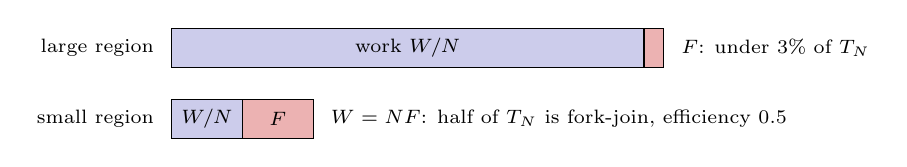
\begin{tikzpicture}[font=\scriptsize, x=1cm, y=1cm]
  \node[anchor=east] at (0,1.5) {large region};
  \draw[fill=native!20] (0.1,1.25) rectangle ++(6.0,0.5) node[midway] {work $W/N$};
  \draw[fill=chrome!30] (6.1,1.25) rectangle ++(0.25,0.5);
  \node[anchor=west] at (6.45,1.5) {$F$: under 3\% of $T_N$};
  \node[anchor=east] at (0,0.6) {small region};
  \draw[fill=native!20] (0.1,0.35) rectangle ++(0.9,0.5) node[midway] {$W/N$};
  \draw[fill=chrome!30] (1.0,0.35) rectangle ++(0.9,0.5) node[midway] {$F$};
  \node[anchor=west] at (2.0,0.6) {$W = NF$: half of $T_N$ is fork-join, efficiency 0.5};
\end{tikzpicture}
\caption{The fork-join model $T_N = W/N + F$. The work of a region divides
by $N$; its fixed cost $F$ does not, and $F$ is six to ten times larger in
the browsers.}
\Description{Two bars: a long bar of work with a small fork-join part, and a short bar where work and fork-join are equal.}
\label{fig:forkjoin-model}
\end{figure}

\begin{itemize}[leftmargin=1.5em]
\item \emph{No size measured reached break-even.} The speedup is above 1 at
every size and thread count, in every environment: even at 512$^2$ eight
threads give 3.4 natively and 1.9 in the browsers for the filter.
\item \emph{Worth it at half the ideal speedup.} At $N=8$ the efficiency
crosses 0.5 at a side of 613 natively and about 995 in both browsers for
the filter (Table~\ref{tab:cutoff-estimates}): 125~\textmu s of sequential
work natively, 396 in Chrome and 459 in Firefox. A region must hold about
three to four times more work in a browser than natively before eight
threads pay half of what they could.
\item \emph{The fork-join model} (Figure~\ref{fig:forkjoin-model}). $T_N = W/N + F$, with $W$ the work of a
region and $F$ the warm fork-join cost of these campaigns' calibration
(10.8, 105 and 60~\textmu s), predicts efficiency 0.5 at $W = NF$: 86, 840
and 480~\textmu s. The measured 125, 396 and 459 agree for Firefox, are 1.5
times the model natively and half of it in Chrome: the calibration's
broadcast is a barrier that every worker must run and overstates what an
ordinary region pays in Chrome. The model is a guide, not a fit.
\item \emph{The 100:1 rule.} A common rule asks that the fork overhead be
under 1\% of a region. At 8192$^2$ the warm fork-join is 0.33\% of $T_8$
natively, 1.4\% in Firefox and 2.7\% in Chrome; by that rule the browsers
would need images of about 10\,000$^2$ and 14\,500$^2$, larger than this
study measured.
\end{itemize}

\paragraph{The sizes are lower bounds for a single call.} With repeated
passes the workers are still awake between passes, which a single call does
not enjoy. Two native control campaigns ran one pass per sample: at 512$^2$
the filter on eight threads takes 33.0~\textmu s per call against
25.8~\textmu s per pass with 256 passes, and at 2048$^2$ 330 against
192~\textmu s, a speedup of 4.56 against 6.86 (the local histogram barely
changes there, 235 against 229~\textmu s). A program that calls a parallel
region once, cold, needs more work per region than the table says.

\clearpage
\subsection{Inside a region: the grain}
\label{sec:grain}

The other half of the question is the size of a task inside one region.
The grain sweeps (5400 runs at $N=8$) give every task a fixed size, in
powers of two, from one row or 1~KB up to one task per thread, with Rayon's
adaptive split as the reference (Table~\ref{tab:grain-best},
Figures~\ref{fig:grain} and~\ref{fig:grain-all}).

\begin{figure}[tbp]
\centering
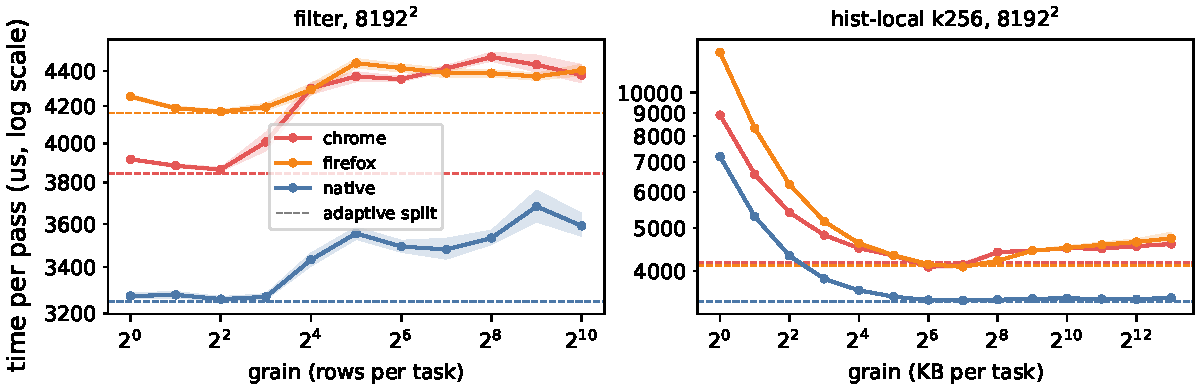
\includegraphics[width=0.8\linewidth]{../figures/grain-ucurve-8192.pdf}
\caption{Grain sweep at 8192$^2$, $N=8$: time per pass against the task
grain (log-log, 95\% CI); dashed: Rayon's adaptive split.}
\Description{Time per pass against task grain for the filter and the local histogram at 8192 squared, one line per environment.}
\label{fig:grain}
\end{figure}

\begin{figure}[tbp]
\centering
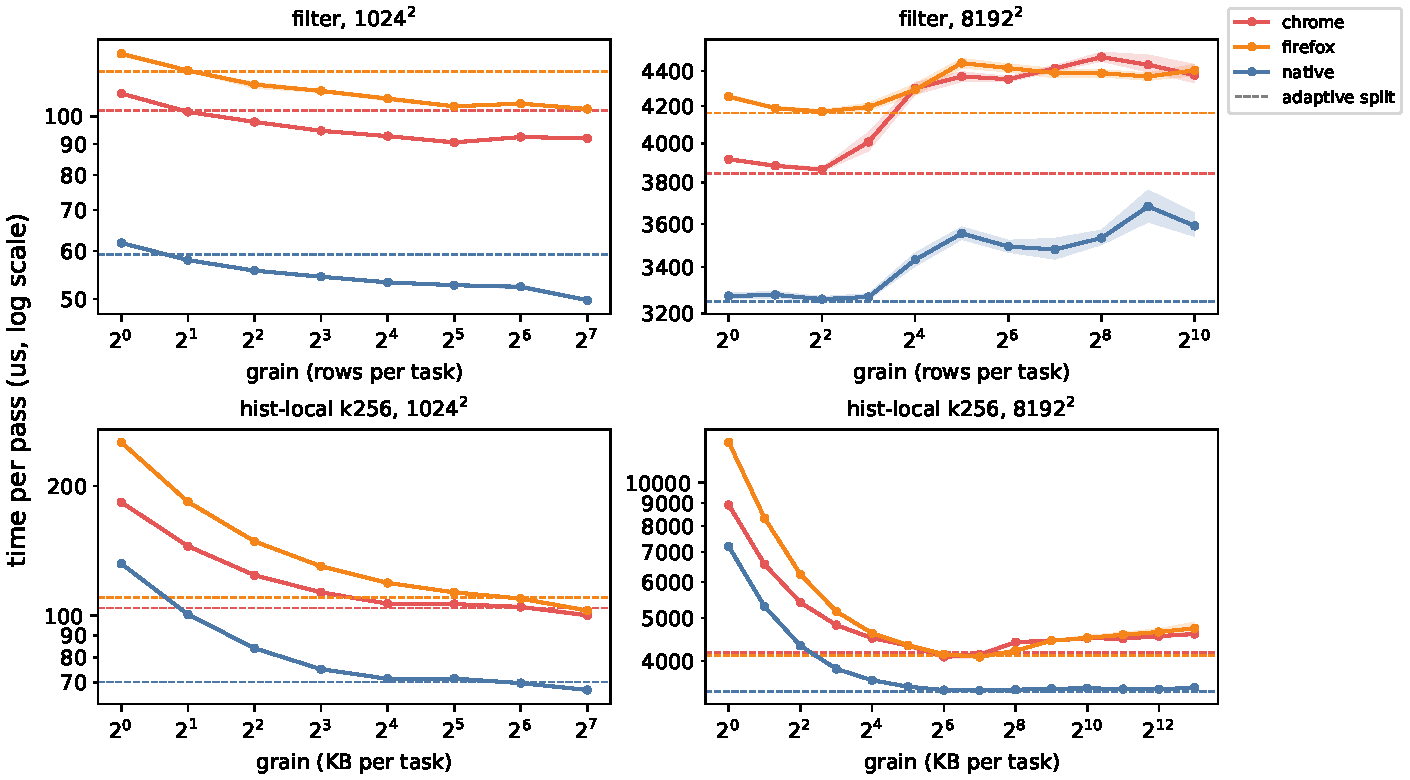
\includegraphics[width=\linewidth]{../figures/grain-ucurve.pdf}
\caption{Grain sweeps at both sizes and for every workload swept.}
\Description{Time per pass against task grain at 1024 squared and 8192 squared.}
\label{fig:grain-all}
\end{figure}

\begin{table}[htbp]
\caption{Grain sweeps at $N=8$: the best fixed grain (rows for the filter, KB for the histograms), its time per pass in \textmu s, the flat region (grains whose interval overlaps the best), Rayon's adaptive split over the best, and the cost of one task in ns with its 95\,\% interval.}\label{tab:grain-best}
\centering\footnotesize
\begin{tabular}{lllrrcrc}
\toprule
Side & Workload & Environment & Best & Time & Flat & Adaptive & Task cost \\
\midrule
1024$^2$ & filter & Chrome & 32 & 90.2 & 32 to 32 & 1.128 & 149 [143, 155] \\
1024$^2$ & filter & Firefox & 128 & 101.9 & 128 to 128 & 1.162 & 199 [191, 207] \\
1024$^2$ & filter & Native & 128 & 50.1 & 128 to 128 & 1.183 & 93 [89, 96] \\
1024$^2$ & local, $k$=256 & Chrome & 128 & 100.5 & 128 to 128 & 1.042 & 641 [631, 650] \\
1024$^2$ & local, $k$=256 & Firefox & 128 & 102.6 & 128 to 128 & 1.056 & 1197 [1189, 1205] \\
1024$^2$ & local, $k$=256 & Native & 128 & 67.5 & 128 to 128 & 1.029 & 504 [498, 510] \\
8192$^2$ & filter & Chrome & 4 & 3848.9 & 2 to 4 & 0.999 & 83 [48, 118] \\
8192$^2$ & filter & Firefox & 4 & 4190.8 & 2 to 8 & 0.996 & 85 [33, 137] \\
8192$^2$ & filter & Native & 4 & 3248.4 & 2 to 4 & 1.002 & 22 [6, 35] \\
8192$^2$ & atomic, $k$=256 & Chrome & 1 & 209470.4 & 1 to 8 & 1.004 & - \\
8192$^2$ & atomic, $k$=256 & Firefox & 4096 & 392514.2 & 512 to 8192 & 1.001 & 537 [481, 592] \\
8192$^2$ & atomic, $k$=256 & Native & 1 & 413763.2 & 1 to 128 & 1.002 & - \\
8192$^2$ & local, $k$=256 & Chrome & 64 & 4094.2 & 64 to 128 & 1.027 & 598 [589, 606] \\
8192$^2$ & local, $k$=256 & Firefox & 128 & 4071.2 & 64 to 128 & 1.010 & 1010 [1003, 1017] \\
8192$^2$ & local, $k$=256 & Native & 128 & 3434.5 & 128 to 256 & 0.995 & 461 [460, 462] \\
\bottomrule
\end{tabular}
\end{table}


\begin{itemize}[leftmargin=1.5em]
\item \emph{A U-curve, as expected.} For the local histogram at 8192$^2$,
tasks of 1~KB cost 2.1 times the best natively, 2.2 times in Chrome and 3.0
times in Firefox: each task builds and merges a 2~KB table. One task per
thread costs 1.01 times natively and 1.11 to 1.16 times in the browsers:
nothing is left to steal when a thread falls behind. For the filter the
curve is shallow: one row per task costs 0.5\% to 1.7\% more than the best,
and 1024 rows per task 7\% to 13\% more.
\item \emph{The best grain is the same in the three environments}: 4 rows
for the filter, 64 to 128~KB for the histogram. The browsers' fork-join is
six to ten times native's, yet their best grain is not coarser, because
what a task pays is not the region's fork-join but the cost of one task:
0.46~\textmu s natively, 0.60 in Chrome and 1.0 in Firefox for the
histogram. The 100:1 rule lands in the flat region when applied to that
cost (110, 117 and 201~KB).
\item \emph{Rayon's adaptive split is within 3\% of the best fixed grain at
8192$^2$} (0.995 to 1.027 times) and 3\% to 18\% slower at 1024$^2$. The
main campaign's use of the adaptive split costs it nothing at its size.
\item \emph{The atomic histogram hardly depends on the grain}: at $k=256$
its time over fifteen grains stays within 0.3\% of the best natively, 0.6\%
in Chrome and 1.3\% in Firefox. Its time is set by contention for the
counters. This also bounds what the v3 change to its task code could have
moved.
\end{itemize}
One feature is unexplained: between grains of 8 and 16 rows the filter
steps up by 4\% natively, 7\% in Chrome and 2\% in Firefox.

\section{Problems Found and Pitfalls of Browser Benchmarking}
\label{sec:problems}

A browser is not a process that waits to be measured: it moves itself,
starts work of its own and updates itself. This section lists every problem
the study met, how it was detected and how it is controlled. Several were
found on earlier builds and fixed before the reported one; they are part of
the method and of the contribution.

\begin{table}[htbp]
\caption{The problems found, in the order they appeared.}
\label{tab:problems}
\centering\scriptsize
\begin{tabular}{rp{0.25\linewidth}p{0.3\linewidth}p{0.32\linewidth}}
\toprule
\# & Problem & How it was detected & Control \\
\midrule
1 & A mask of eight CPUs that is four cores & Review of the CPU numbering before measuring & SMT off, one CPU per core, checked per run \\
2 & Background work on the measured cores & Design review & Shield, quiet mode, foreign CPU time per run \\
3 & Asymmetric background services between the browsers & Review of the launch settings & The same services off in both \\
4 & Chrome's browser process leaves the CPU mask & A sampler of every thread's allowed CPUs & No session bus for the browser; escaped processes counted per run and rejected \\
5 & Firefox still starting up during the measurement & Bursty iterations; a pilot with and without delay & A 3 s start delay in every browser run \\
6 & A slow first browser launch & Launch times on a new machine & One discarded launch per browser before the plan \\
7 & A command run during a campaign & One run over the foreign CPU threshold & Nothing else is started during a campaign \\
8 & Our own asymmetries in RQ2 & Review of the measured path against its machine code & A new build; everything measured again \\
9 & The pinned Firefox updated itself & Strict validation of the recorded version & An enterprise policy, the version read from the install, a check before every campaign \\
10 & A degraded core & Crashes pinned to one core & Measure only on the prepared machine; per-core check; the build made twice \\
11 & A wrong computation without a crash & A type error inside a library on valid data & Analysis pinned away from the core; tables regenerated on another machine \\
12 & A new workload changed another's machine code & The codegen comparison & The sequential filter has its own copy of the row code \\
13 & A gate criterion failed twice & The gate & A recorded decision before the campaign; the effect measured \\
14 & Whole-run counters are mostly not the loop & A sanity check against the listing & Counters by the difference of two pass counts \\
\bottomrule
\end{tabular}
\end{table}

\paragraph{4. Chrome escapes the mask.} During the mask pilot a sampler read
the allowed CPUs of every thread and showed Chrome's browser process on the
E-cores. Chrome asks the desktop session, through the D-Bus session bus, to
move it into its own systemd scope, which is outside the run's scope and
its mask. Firefox's processes all stayed inside, so the two browsers were
not confined alike. Without the session bus address every Chrome process
stays in the run scope. Each run now counts the processes of its browser
found outside its scope, and strict validation rejects a run with any. The
renderer, where the WASM and its workers run, had stayed on the P-cores
throughout, and the pilots taken before the fix were repeated where their
decision could depend on it. A process-level mask is a request that a
process can undo.

\paragraph{5. Firefox's start-up work.} With a fresh profile on every run,
the page starts measuring while the browser is still starting. For short
iterations at eight threads this made Firefox's local histogram 1.32 times
slower and bursty, and produced a ``knee'' at seven and eight threads that
looked like oversubscription and was first read as such. A 3~s delay before
the page creates its worker removes both. A scaling artefact at high $N$
that comes from start-up is the kind of effect that would be reported as a
result of the engine.

\paragraph{7. Activity during a campaign.} On the second build one run
exceeded the foreign-CPU threshold because a version-control command ran
during a campaign; the run was repeated. Since then campaigns start quiet
mode themselves. For the v3 campaigns the coding assistant used during
development was kept alive, confined to the E-cores, instead of being
stopped (stopping it also froze the terminals it ran in for the 14 hours of
the main campaign), under the rule that no command is started while a
campaign runs. A rule cannot be checked, but what each run records can: the
load average and the foreign CPU time of the v3 main campaign
(Section~\ref{sec:quality}) are those of the v2 main campaign, in which the
assistant was stopped (medians 3.00 and 3.19, maxima of foreign CPU time
0.205 and 0.222~s). That is evidence of the same quiet, not proof that
nothing ran.

\paragraph{8. Our own asymmetries.} The RQ2 numerator paid a bounds check
per pixel that the denominator did not; and the final step of a histogram
was timed in some variants only. Neither would show in any quality check,
since every checksum was right. They were found by reading the measured
path against its disassembly. The fix was not a correction of the numbers
but a new build and a second full measurement
(Section~\ref{sec:builds-history}).

\paragraph{9. Firefox updates itself.} The profile setting that turns
automatic updates off does not stop the download or the update on the next
start. During the exploratory campaigns of the second build the pinned
Firefox 158.0 replaced itself with 160.0. Because every run records the
version of the binary it launched, strict validation rejected all 2640
affected runs; they were set aside and repeated on 158.0. Only an
enterprise policy file stops the updater; the installer now writes it, reads
the version from the install itself, and a campaign refuses to start with
another version. In v3 no campaign was affected and every environment is
interleaved in every campaign. Chrome for Testing has no updater.

\paragraph{10 and 11. The degraded core.} Section~\ref{sec:core}. The lesson
beyond this machine: a crash is the easy failure. A core that computes
wrongly without crashing is caught only by checksums (in the measured
code), by reproducible builds (in the compiler) and by regenerating results
elsewhere (in the analysis).

\paragraph{12. Code that did not change, changed.} Adding a second caller
to a function that the compiler had inlined changed the machine code of the
parallel filter, whose source was untouched (Section~\ref{sec:codegen}). A
comparison of two builds is a comparison of two instruction streams;
without a tool that compares them, this would have been measured as noise
or, worse, as a result.

\paragraph{14. Counters of a whole run.} Section~\ref{sec:why-rq1}: per-pixel
counters of a browser run were three to eight times what the loop executes,
because a run is also a browser start, an input generation and checksums.
Only the difference between two campaigns that differ in the amount of loop
work isolates the loop.

\paragraph{For benchmarkers.} A CPU mask, a fresh profile and a pinned
version do not by themselves confine, quiet and freeze a browser. What made
these problems visible was recording the state with every run (the allowed
CPUs, the version, the foreign CPU time, the checksum) and rejecting runs
by rules fixed in advance.

\section{Threats to Validity}
\label{sec:threats}

Each item says how it is known: \emph{measured} (a number from the data),
\emph{recorded} (a fact of the setup) or \emph{not established} (a likely
cause that no data here isolates).

\subsection{Internal validity}

\begin{itemize}[leftmargin=1.5em]
\item \emph{One P-core is degraded.} Measured: on the prepared machine it
gives the right checksum and the time of the other cores, and it took 9 of
the 30 native one-thread filter runs with a median 1.0003 times the
configuration's. Not established: that it never slows down within a run;
ten pinned runs in one session do not rule out a core that is slow now and
then. At $N=8$ every run of every environment uses it.
\item \emph{Thread placement is left to the kernel}, because a browser
cannot pin threads. Measured: the shared-atomic cells at $k=1$ land on
several time levels from run to run, which makes them the widest cells
(Section~\ref{sec:levels}). Not established: what sets the level of a run.
\item \emph{The layers below the crate differ} (Section~\ref{sec:builds}):
WASM-only flags, a rebuilt standard library, other locks inside Rayon, idle
workers that spin instead of yielding, and the engines' compilers. They are
the environment under study; ``the same code'' is claimed for the crate
only.
\item \emph{The compiler tier.} Measured: in every cell of the tier
campaign the browser as shipped equals its optimizing-only arm after the
warm-up, so the campaigns measure optimized code. Recorded: the listings of
V8's code come from diagnostic runs with other flags.
\item \emph{Slow early iterations in one Firefox cell.} Measured: one or
two of the first three measured iterations of the local histogram at $k=1$,
$N=8$ are about 10\% slower, after 71 warm-up iterations, in 27 of 30 runs;
the run value moves by about 0.1\%. This cell is the control of one primary
contrast. Not established: what they are; they come with the optimizing
compiler's code.
\item \emph{The fork-join calibration has 20 samples and a coarse clock.}
Recorded: with a 20~\textmu s clock Firefox's warm fork-join reads 0 at
$N \leq 4$.
\item \emph{Browser threads share the measured cores.} Recorded: Firefox
reports a hardware concurrency of 32 and Chrome of 8, so Firefox sizes its
helper threads for the whole machine while confined to eight cores. Not
established: how much CPU, cache or memory bandwidth they take during a
timed iteration. With the start delay no browser shows a knee at eight
threads.
\item \emph{A coding assistant was alive during the campaigns}, confined to
the E-cores under a no-command rule. Measured: load and foreign CPU time
equal those of a campaign without it. Not established: that nothing ran on
the other cores that shares the cache.
\item \emph{Frequency is not known during a run.} Recorded: turbo off and
the governor fixed. Measured: the kernel's frequency sample read 1154 to
3201~MHz on cores that had just run at full speed, so it cannot tell a slow
core from one read while going idle; it is recorded and not used.
\item \emph{Memory growth.} Measured: the native filter's memory grows by
exactly 65\,536~KiB in the warm-up and by nothing in the measured phase at
one and two threads, and by a few KiB (stack pages) with more.
\item \emph{The native runs have no start delay} and the browsers wait 3~s
idle. It affects $T_1$ and $T_N$ of an environment alike.
\item \emph{The counters of the loop} come from two campaigns run one after
the other, so the pass count is confounded with the block.
\end{itemize}

\subsection{Construct validity}

\begin{itemize}[leftmargin=1.5em]
\item \emph{RQ2 is a ratio of ratios.} Measured: the environment gap of the
local control moves it as much as the atomics do
(Section~\ref{sec:decomposition}); it is reported with both factors and
with the ratio of the excesses.
\item \emph{The control is not neutral in $k$.} At small $k$ the local
histogram is itself a dependent chain. The contrast compares within one
$k$, never across.
\item \emph{Speedup is relative to a pool of one thread.} Measured: that
pool is within $-7$\% to $+5$\% of sequential code in every environment
(Section~\ref{sec:sequential}); the time over native and the absolute
speedup are reported next to it.
\item \emph{The efficiency dip at $N=6$ and 7 is not explained.} Measured:
it appears in every environment, and fixed grains do not remove it
(Section~\ref{sec:dip}).
\item \emph{The atomic code differs between engines}, which is the finding
of RQ2 and also a limit of its name: what is compared is ``shared atomic
counters as each compiler emits them'', not one instruction in three places.
\item \emph{The cutoff sizes are lower bounds for a single call}
(Section~\ref{sec:cutoff}).
\end{itemize}

\subsection{Statistical conclusion validity}

\begin{itemize}[leftmargin=1.5em]
\item \emph{Precision.} With 30 runs the primary 99.5\% intervals are
within $\pm$2\% for RQ1 and $\pm$7\% for RQ2 (the widest, Chrome at $k=1$).
The two non-rejections are bounded by their intervals, about 1\% and 6\%,
and are not equalities.
\item \emph{Percentile bootstrap intervals over 30 runs} run slightly
narrow at the 99.5\% level; the plan fixed them before the data.
\item \emph{The points of one speedup curve share their $T_1$}, so an error
in $T_1$ shifts the whole curve.
\item \emph{The smallest rejected effect is 3\%} (Firefox at $k=4$). On the
earlier build the Firefox values at $k=4$ and 256 moved between two builds
by more than that, so this rejection is not read as an effect of the
environment; the reading of Firefox rests on the two factors.
\item \emph{This is a replication whose first results were known.} The
rule for adopting the build read only counts of runs, and the analysis
plan did not change.
\item \emph{Exploratory results} use uncorrected 95\% intervals and decide
nothing. The robustness check was added after the first primary results
existed.
\end{itemize}

\subsection{External validity}

\begin{itemize}[leftmargin=1.5em]
\item \emph{One machine, one compiler version, one version of each
browser.} The RQ2 finding is about the code V8 155 emits for an atomic add;
another version may emit another sequence, and the same engine with its
other compiler already does.
\item \emph{P-cores only, turbo off.} The hybrid campaign shows what
E-cores add; nothing here describes turbo.
\item \emph{Every primary cell lives in memory, not in cache}: 128~MiB for
the filter's two images and 64~MiB for the histograms, against a 36~MB
last-level cache. The explanation of RQ1 is about this regime. The in-cache
regime appears only in the cutoff campaigns.
\item \emph{Inputs are uniform random values} with no spatial structure,
one seed, one size.
\item \emph{Two workloads}, both data-parallel loops over an image. Nothing
here covers locks, channels, allocation-heavy code (beyond one sort) or
irregular parallelism.
\item \emph{Headless browsers} on an idle machine; a pilot bounds the
difference to headful at 0.3\%.
\end{itemize}

\section{Reproducibility}
\label{sec:reproducibility}

\paragraph{Provenance.} Every number of this report comes from one build,
the tag \code{measured/v3} (commit \code{ac65af6a}), built twice from
scratch with equal digests. The repository holds that build's code, the raw
runs of every campaign (one CSV and one context file per run, the campaign's
specification and its journal in execution order, the discarded first
launches and the state of the machine at the start), the derived tables,
the probes with their code and data, the checks that are not results (the
per-core check, the two gates), the progress logs of the measuring session,
and one decision record per design decision. The data of the earlier build
are kept at a tag, and the evidence older than that (pilot runs, one-off
probes) in a folder of its own.

\paragraph{From runs to tables.} One command regenerates every table and
figure from the raw runs. A second regenerates them and fails if any line
of any table differs from the committed one (only the commit and the
creation time of a table's side file may change); the continuous
integration runs it on another machine whenever the analysis, the harness
or the data change. The bootstrap is seeded, so the intervals are
reproducible to the digit. The tables of this report are written from the
committed tables by a script, so no number of a table is typed by hand.

\paragraph{From source to runs.} Development and tests run anywhere; a
campaign of the study needs more:
\begin{itemize}[leftmargin=1.5em]
\item Linux with systemd and a graphical session (the browsers start
headless but need the session's display variables), and administrator
rights for the environment setup and for the run scopes.
\item The CPU layout of this study is written in two places that must
change together, the masks of the make targets and of every campaign
specification; they describe an i9-14900KF.
\item Time: the main campaign is 5310 runs and 14 hours, and it resumes if
stopped; all campaigns together took about 56 hours of machine time.
\item The pinned toolchain, crates and browser builds, which the setup
target installs without administrator rights, with the browsers' archives
checked against pinned digests.
\end{itemize}

\paragraph{Checks that run on every change.} Formatting, lints and tests of
the crate for both targets; the WASM package built from a clean checkout;
SIMD parity on the final native binary and the final WASM module; every
workload run in both browsers with checksums and input fingerprints
compared with native; the tests of the harness, the analysis and the
scripts under strict typing; the structure of the decision records; and
the regeneration of the tables.

\paragraph{What cannot be reproduced exactly.} The times depend on this
machine, including its degraded core. Another machine should reproduce the
decisions and the shapes, not the milliseconds. The effect of RQ2 depends
on the engine versions; the native probe (one C file) reproduces its
mechanism on any x86 machine without a browser.

\section{Discussion and Conclusions}
\label{sec:discussion}

\subsection{RQ1}

\emph{How do relative speedup and efficiency of the same parallel code
evolve with the number of threads, natively and in WASM in the browser?}

With enough work per parallel region, the same way. On a loop with no
synchronization the efficiency falls slowly with $N$, to 0.87 at eight
threads natively and in Chrome and 0.92 in Firefox; Chrome's speedup is
within about 1\% of native's, and the browser over native time ratio does
not grow with $N$, in strong and in weak scaling. A loop that does not
touch shared memory scales almost ideally in the three environments (the
local histogram, 0.98 to 1.06).

WASM costs a constant factor per thread, 1.17 in Chrome and 1.36 in Firefox
on the filter, measured here as a third more instructions per pixel run at
different rates. That factor divides with the work. What does not divide is
the fixed cost of a parallel region, six to ten times larger in the
browsers: negligible for regions of milliseconds, half of the time for
regions of about 0.4~ms at eight threads.

The one significant RQ1 difference, Firefox's higher speedup, is not
evidence that a browser runs threads better. The sub-linear speedup of the
filter is not a serial fraction (the timed region has none) but a cost of
eight threads sharing memory, and a slower loop asks less of the memory:
across three builds and three environments, the faster one thread reads
memory the less eight threads gain. Firefox is the slowest environment at
every thread count. This explanation is supported by counters, by the SIMD
builds, natively by the image size, and by one intervention inside each
engine; none of them intervenes on the memory itself, and about half of the
native loss is time outside the loop that was not measured.

\subsection{RQ2}

\emph{To what extent does synchronization between threads affect the
scalability gap between WASM and native?}

It depends on the engine, and on how the contention is spread. In Chrome,
relative to the lock-free control, shared atomic counters cost 1.4 to 2.3
times what they cost natively when contention is concentrated, and 0.42
times when it is spread over 256 counters. In Firefox they cost what they
cost natively in absolute time; its ratios below 1 come from a slower
control, not from cheaper synchronization.

The difference is a compiler's choice, not a property of WASM threads.
Memory ordering is not the reason: WASM atomics are sequentially
consistent~\cite{watt2019}, but on x86 an atomic add costs the same
whatever ordering is asked~\cite{schweizer2015}. V8's optimizing compiler
turns an atomic add whose result is unused into a compare-and-swap loop.
That sequence is slower uncontended, is retried once in four adds under
concentrated contention, and is faster when eight cores spread over 256
lines. A native program with the same sequence reproduces Chrome's times in
both directions; the same engine with its baseline compiler, and the other
engine, show no penalty at $k=1$. One source and one set of flags do not
give one instruction stream, so a statement about ``WASM atomics'' is a
statement about an engine version.

\subsection{For developers}

\begin{itemize}[leftmargin=1.5em]
\item Porting a data-parallel loop to WASM threads keeps its scaling and
costs a constant factor; expect 1.2 to 1.4 times the native time on loops
like these.
\item Keep parallel regions coarse. At eight threads a region needs about
0.4 to 0.5~ms of sequential work in a browser to get half the ideal
speedup, three to four times what native code needs, and more if it is
called once and cold.
\item Inside a region (Section~\ref{sec:grain}), Rayon's adaptive split is within 3\% of the best
fixed grain at these sizes in the three environments; there is no reason
to tune the grain per environment.
\item Avoid shared counters, as natively: they do not scale anywhere.
Privatize and merge. Where atomics are unavoidable, give each its own cache
line, and do not assume that their cost in one engine predicts another.
\end{itemize}

\subsection{For benchmarkers}

\begin{itemize}[leftmargin=1.5em]
\item A CPU mask, a fresh profile and a pinned version do not by
themselves confine, quiet and freeze a browser. Record the state with every
run and reject runs by rules fixed in advance.
\item Read the machine code. Both findings of this study, and two of our
own mistakes, were visible only there.
\item A relative speedup needs its baseline: a slower environment can
scale better because it is slower.
\item Whole-run hardware counters of a browser are mostly not the code
under test.
\item Write the prediction before the test. One of ours failed in part,
and it is the most informative line of Section~\ref{sec:why-rq2}.
\end{itemize}

\subsection{What stays open}

The mechanism that makes a compare-and-swap loop faster than a locked add
when eight cores spread over 256 padded counters. Why SpiderMonkey's filter
loop, as long as V8's, runs fewer instructions per cycle, and why its local
histogram misses more caches with one thread. What Chrome loses outside the
loop at eight threads, and whether the idle and wake path of the WASM
thread pool is what makes the browsers' fork-join slower. The efficiency
dip at six and seven threads. What sets the state of contention of a run
at $k=1$. The slow early iterations of one Firefox cell. And everything
outside this design: other machines, turbo, other engine versions, locks
and irregular parallelism.

\subsection{Conclusion}

The same Rust/Rayon code scales in the browser as natively when each
parallel region has enough work: WASM threads cost a roughly constant
factor and a slower fork-join, and where a browser scales better it is
because its code is slower on a memory-bound loop. Shared atomics widen the
gap in Chrome under concentrated contention and narrow it under spread
contention; Firefox is never worse than native. The cause is V8's
compare-and-swap loop for an atomic add, reproduced natively and absent
from V8's other compiler. The study was measured twice in full; the second
measurement, with its corrections and a rule for adopting it fixed in
advance, gives the same ten decisions as the first.


\paragraph{Use of AI} Written with Claude (Anthropic) from the project's
data and decision records.

\bibliographystyle{ACM-Reference-Format}
\bibliography{../bib/referencias}

\appendix
\section{Tables test}
{\small
\begin{longtable}{llcc}
\caption{Main campaign: time in the browser over the native time at the same $N$, with its 95\,\% bootstrap interval (exploratory).}\label{tab:absolute} \\
\toprule
Workload & $N$ & Chrome & Firefox \\
\midrule
\endfirsthead
\toprule
Workload & $N$ & Chrome & Firefox \\
\midrule
\endhead
\bottomrule
\endfoot
filter & 1 & 1.172 [1.167, 1.177] & 1.363 [1.356, 1.372] \\
filter & 2 & 1.174 [1.166, 1.184] & 1.36 [1.348, 1.373] \\
filter & 4 & 1.189 [1.184, 1.195] & 1.362 [1.347, 1.381] \\
filter & 6 & 1.186 [1.18, 1.191] & 1.337 [1.326, 1.348] \\
filter & 7 & 1.189 [1.184, 1.194] & 1.316 [1.307, 1.326] \\
filter & 8 & 1.177 [1.172, 1.183] & 1.292 [1.28, 1.309] \\
\midrule
atomic, $k$=1 & 1 & 1.839 [1.839, 1.839] & 1 [1, 1] \\
atomic, $k$=1 & 2 & 2.251 [2.187, 2.316] & 1.035 [0.9963, 1.076] \\
atomic, $k$=1 & 4 & 2.264 [2.137, 2.396] & 1.009 [0.9607, 1.058] \\
atomic, $k$=1 & 6 & 2.23 [2.119, 2.345] & 1.037 [0.988, 1.086] \\
atomic, $k$=1 & 7 & 2.12 [2.022, 2.225] & 1.017 [0.9744, 1.062] \\
atomic, $k$=1 & 8 & 2.206 [2.107, 2.308] & 1.026 [0.9866, 1.065] \\
\midrule
atomic, $k$=4 & 1 & 1.551 [1.549, 1.554] & 1 [1, 1] \\
atomic, $k$=4 & 2 & 1.349 [1.329, 1.37] & 1.015 [1, 1.031] \\
atomic, $k$=4 & 4 & 1.583 [1.567, 1.6] & 0.9939 [0.9821, 1.006] \\
atomic, $k$=4 & 6 & 1.791 [1.775, 1.808] & 0.9823 [0.9727, 0.9925] \\
atomic, $k$=4 & 7 & 1.874 [1.858, 1.89] & 0.9949 [0.9855, 1.004] \\
atomic, $k$=4 & 8 & 1.909 [1.892, 1.925] & 0.9837 [0.9751, 0.9928] \\
\midrule
atomic, $k$=16 & 1 & 1.287 [1.286, 1.288] & 1.001 [1.001, 1.001] \\
atomic, $k$=16 & 2 & 1.149 [1.137, 1.161] & 1.034 [1.023, 1.045] \\
atomic, $k$=16 & 4 & 1.395 [1.379, 1.412] & 1.017 [1.003, 1.032] \\
atomic, $k$=16 & 6 & 1.593 [1.585, 1.602] & 1.008 [1.001, 1.015] \\
atomic, $k$=16 & 7 & 1.687 [1.678, 1.695] & 1.008 [1.002, 1.014] \\
atomic, $k$=16 & 8 & 1.78 [1.772, 1.789] & 1.007 [1.002, 1.013] \\
\midrule
atomic, $k$=256 & 1 & 1.085 [1.085, 1.085] & 1.001 [1.001, 1.001] \\
atomic, $k$=256 & 2 & 0.8694 [0.869, 0.8699] & 0.9345 [0.9343, 0.9348] \\
atomic, $k$=256 & 4 & 0.4282 [0.4251, 0.4314] & 0.5756 [0.5718, 0.5796] \\
atomic, $k$=256 & 6 & 0.456 [0.4546, 0.4575] & 0.7443 [0.7423, 0.7464] \\
atomic, $k$=256 & 7 & 0.4831 [0.4818, 0.4845] & 0.866 [0.8635, 0.8686] \\
atomic, $k$=256 & 8 & 0.5074 [0.5068, 0.508] & 0.9479 [0.9468, 0.949] \\
\midrule
local, $k$=1 & 1 & 0.973 [0.9724, 0.9736] & 1.005 [1.004, 1.005] \\
local, $k$=1 & 2 & 0.9733 [0.9727, 0.9739] & 1.006 [1.006, 1.006] \\
local, $k$=1 & 4 & 0.9759 [0.9753, 0.9766] & 1.014 [1.014, 1.015] \\
local, $k$=1 & 6 & 0.9813 [0.9783, 0.9842] & 1.01 [1.007, 1.013] \\
local, $k$=1 & 7 & 0.9743 [0.9723, 0.9763] & 1.008 [1.007, 1.01] \\
local, $k$=1 & 8 & 0.9762 [0.9755, 0.977] & 1.015 [1.014, 1.017] \\
\midrule
local, $k$=4 & 1 & 1.07 [1.069, 1.071] & 1.024 [1.023, 1.025] \\
local, $k$=4 & 2 & 1.068 [1.067, 1.069] & 1.022 [1.021, 1.023] \\
local, $k$=4 & 4 & 1.075 [1.072, 1.078] & 1.016 [1.014, 1.018] \\
local, $k$=4 & 6 & 1.084 [1.079, 1.089] & 1.023 [1.018, 1.029] \\
local, $k$=4 & 7 & 1.088 [1.083, 1.093] & 1.018 [1.013, 1.022] \\
local, $k$=4 & 8 & 1.078 [1.074, 1.082] & 1.015 [1.011, 1.019] \\
\midrule
local, $k$=16 & 1 & 1.244 [1.24, 1.248] & 1.273 [1.27, 1.276] \\
local, $k$=16 & 2 & 1.211 [1.207, 1.215] & 1.224 [1.221, 1.228] \\
local, $k$=16 & 4 & 1.224 [1.22, 1.228] & 1.242 [1.239, 1.246] \\
local, $k$=16 & 6 & 1.258 [1.25, 1.266] & 1.261 [1.255, 1.268] \\
local, $k$=16 & 7 & 1.255 [1.242, 1.266] & 1.26 [1.253, 1.267] \\
local, $k$=16 & 8 & 1.249 [1.235, 1.264] & 1.212 [1.203, 1.221] \\
\midrule
local, $k$=256 & 1 & 1.232 [1.225, 1.243] & 1.273 [1.256, 1.298] \\
local, $k$=256 & 2 & 1.231 [1.224, 1.243] & 1.27 [1.256, 1.286] \\
local, $k$=256 & 4 & 1.244 [1.238, 1.251] & 1.279 [1.267, 1.29] \\
local, $k$=256 & 6 & 1.248 [1.233, 1.262] & 1.258 [1.245, 1.269] \\
local, $k$=256 & 7 & 1.254 [1.246, 1.263] & 1.272 [1.262, 1.281] \\
local, $k$=256 & 8 & 1.22 [1.202, 1.238] & 1.19 [1.177, 1.205] \\
\end{longtable}
}

\begin{table}[htbp]
\caption{One-thread filter runs of the main campaign split by the CPU with the most busy time: runs, their median and slowest run over the configuration's median, and that CPU's share of the run's busy time. CPU 12 is the degraded core.}\label{tab:core-split}
\centering\small
\begin{tabular}{llrrrrr}
\toprule
Environment & Workload & CPU & Runs & Median & Max & Busy share \\
\midrule
Chrome & filter & 12 & 12 & 1.0026 & 1.0144 & 0.643 \\
Chrome & filter & 14 & 18 & 0.9986 & 1.0189 & 0.595 \\
Chrome & filter-seq & 12 & 16 & 1.0043 & 1.0190 & 0.811 \\
Chrome & filter-seq & 14 & 14 & 0.9938 & 1.0216 & 0.807 \\
Firefox & filter & 12 & 11 & 1.0020 & 1.0426 & 0.471 \\
Firefox & filter & 14 & 19 & 0.9997 & 1.0622 & 0.485 \\
Firefox & filter-seq & 12 & 12 & 1.0052 & 1.0525 & 0.562 \\
Firefox & filter-seq & 14 & 18 & 0.9997 & 1.0352 & 0.559 \\
Native & filter & 12 & 9 & 1.0003 & 1.0029 & 0.801 \\
Native & filter & 14 & 21 & 0.9997 & 1.0049 & 0.706 \\
Native & filter-seq & 12 & 22 & 1.0000 & 1.0017 & 0.990 \\
Native & filter-seq & 14 & 8 & 1.0001 & 1.0016 & 0.990 \\
\bottomrule
\end{tabular}
\end{table}

\begin{table}[htbp]
\caption{Hardware counters of the atomic histogram per atomic add (means of 30 runs, counted system-wide on the P-cores for the whole run): cycles, instructions, locked loads, lines taken for writing from another core (RFO HITM), lines read from another core (read HITM) and L2 misses.}\label{tab:counters-atomic}
\centering\small
\begin{tabular}{lllrrrrrr}
\toprule
$k$ & $N$ & Environment & Cycles & Instr. & Lock loads & RFO HITM & Read HITM & L2 miss. \\
\midrule
1 & 1 & Native & 19.1533 & 5.0767 & 0.9992 & 0.0000 & 0.0000 & 0.0008 \\
1 & 1 & Chrome & 37.7201 & 24.1086 & 1.0160 & 0.0006 & 0.0016 & 0.0069 \\
1 & 1 & Firefox & 31.4093 & 33.1235 & 1.0370 & 0.0018 & 0.0053 & 0.0195 \\
\midrule
1 & 8 & Native & 336.0000 & 5.5722 & 1.0003 & 0.2425 & 0.0002 & 0.2177 \\
1 & 8 & Chrome & 680.9191 & 26.7122 & 1.2582 & 0.1956 & 0.2992 & 0.3872 \\
1 & 8 & Firefox & 365.1023 & 34.1941 & 1.0391 & 0.2500 & 0.0058 & 0.2209 \\
\midrule
256 & 1 & Native & 19.1209 & 5.0697 & 0.9986 & 0.0000 & 0.0000 & 0.0006 \\
256 & 1 & Chrome & 25.9478 & 24.0954 & 1.0159 & 0.0006 & 0.0015 & 0.0065 \\
256 & 1 & Firefox & 32.4503 & 33.3375 & 1.0379 & 0.0018 & 0.0052 & 0.0196 \\
\midrule
256 & 8 & Native & 158.3065 & 5.3206 & 0.9990 & 1.0406 & 0.0001 & 0.8015 \\
256 & 8 & Chrome & 85.5763 & 24.5930 & 1.0305 & 0.5171 & 0.7117 & 0.2134 \\
256 & 8 & Firefox & 164.0309 & 33.8173 & 1.0388 & 0.8898 & 0.0057 & 0.7718 \\
\bottomrule
\end{tabular}
\end{table}

\begin{table}[htbp]
\caption{Counters of the loop alone at one thread, per pixel, by the difference of two pass counts (10 runs with one pass and 10 with eight), with 95\,\% bootstrap intervals. LLC and L2 are cache misses.}\label{tab:counters-loop}
\centering\scriptsize
\resizebox{\linewidth}{!}{%
\begin{tabular}{llcccc}
\toprule
Workload & Environment & Instructions & Cycles & LLC misses & L2 misses \\
\midrule
filter & Native & 4.103 [4.098, 4.108] & 1.067 [1.062, 1.072] & 0.01378 [0.01374, 0.01383] & 0.000329 [0.0003247, 0.0003335] \\
filter & Chrome & 5.517 [5.478, 5.539] & 1.243 [1.221, 1.26] & 0.01285 [0.01277, 0.01292] & 0.0003967 [0.0003883, 0.0004042] \\
filter & Firefox & 5.408 [5.371, 5.431] & 1.451 [1.428, 1.473] & 0.01049 [0.01034, 0.01064] & 0.000424 [0.0004113, 0.0004354] \\
\midrule
local, $k$=16 & Native & 2.761 [2.755, 2.767] & 1.359 [1.356, 1.363] & 0.003641 [0.003621, 0.003661] & 0.0004206 [0.0004167, 0.0004239] \\
local, $k$=16 & Chrome & 7.025 [7.02, 7.03] & 1.708 [1.699, 1.718] & 0.003774 [0.003697, 0.003856] & 0.0004188 [0.0004122, 0.0004257] \\
local, $k$=16 & Firefox & 6.819 [6.814, 6.825] & 1.751 [1.745, 1.755] & 0.003558 [0.003474, 0.003644] & 0.0004669 [0.0004556, 0.0004786] \\
\midrule
local, $k$=256 & Native & 2.772 [2.761, 2.785] & 1.294 [1.288, 1.3] & 0.004266 [0.004236, 0.004299] & 0.0004456 [0.00044, 0.0004517] \\
local, $k$=256 & Chrome & 7.004 [6.978, 7.025] & 1.593 [1.564, 1.637] & 0.00307 [0.002981, 0.00317] & 0.0004338 [0.0004246, 0.0004416] \\
local, $k$=256 & Firefox & 6.817 [6.811, 6.822] & 1.701 [1.638, 1.819] & 0.003646 [0.003578, 0.003714] & 0.0004924 [0.0004735, 0.0005083] \\
\bottomrule
\end{tabular}
}
\end{table}

\begin{table}[htbp]
\caption{Cutoff at $N=8$: the image side at which the efficiency crosses 0.5 (interpolated, 95\,\% interval) and the sequential work of that image in \textmu s; then the fork-join model $T_N=W/N+F$ with this campaign's warm fork-join $F$ in \textmu s: the work it predicts for efficiency 0.5, and the side at which $F$ is 1\,\% and 5\,\% of $T_N$.}\label{tab:cutoff-estimates}
\centering\footnotesize
\begin{tabular}{llcrrrrr}
\toprule
Workload & Environment & Side at 0.5 & Work & $F$ & Model & Side 1\,\% & Side 5\,\% \\
\midrule
filter & Native & 613 [610, 616] & 124.9 & 10.8 & 86.1 & 5031 & 2204 \\
local, $k$=256 & Native & 691 [679, 701] & 183.4 & 10.8 & 86.1 & 4595 & 2013 \\
filter & Chrome & 996 [989, 1002] & 395.6 & 105.0 & 840.0 & 14518 & 6360 \\
local, $k$=256 & Chrome & 815 [797, 832] & 324.6 & 105.0 & 840.0 & 12938 & 5668 \\
filter & Firefox & 994 [976, 1009] & 459.4 & 60.0 & 480.0 & 10151 & 4447 \\
local, $k$=256 & Firefox & 858 [840, 873] & 361.9 & 60.0 & 480.0 & 9607 & 4209 \\
\bottomrule
\end{tabular}
\end{table}

{\footnotesize
\begin{longtable}{lllccccc}
\caption{Cutoff campaigns: speedup (efficiency) by image side, with repeated passes per timed sample so that small images clear the clock.}\label{tab:cutoff} \\
\toprule
Workload & $N$ & Environment & 512$^2$ & 1024$^2$ & 2048$^2$ & 4096$^2$ & 8192$^2$ \\
\midrule
\endfirsthead
\toprule
Workload & $N$ & Environment & 512$^2$ & 1024$^2$ & 2048$^2$ & 4096$^2$ & 8192$^2$ \\
\midrule
\endhead
\bottomrule
\endfoot
filter & 2 & Native & 1.890 (0.945) & 1.944 (0.972) & 1.968 (0.984) & 1.913 (0.957) & 1.959 (0.979) \\
filter & 2 & Chrome & 1.900 (0.950) & 1.951 (0.975) & 2.029 (1.014) & 1.914 (0.957) & 1.970 (0.985) \\
filter & 2 & Firefox & 1.877 (0.939) & 1.964 (0.982) & 2.047 (1.023) & 1.935 (0.967) & 1.980 (0.990) \\
filter & 4 & Native & 3.063 (0.766) & 3.622 (0.906) & 3.837 (0.959) & 3.523 (0.881) & 3.775 (0.944) \\
filter & 4 & Chrome & 3.145 (0.786) & 3.610 (0.903) & 3.957 (0.989) & 3.481 (0.870) & 3.741 (0.935) \\
filter & 4 & Firefox & 3.207 (0.802) & 3.697 (0.924) & 4.001 (1.000) & 3.610 (0.902) & 3.817 (0.954) \\
filter & 8 & Native & 3.428 (0.429) & 5.622 (0.703) & 6.860 (0.857) & 7.519 (0.940) & 6.926 (0.866) \\
filter & 8 & Chrome & 1.936 (0.242) & 4.086 (0.511) & 6.528 (0.816) & 6.067 (0.758) & 6.905 (0.863) \\
filter & 8 & Firefox & 1.906 (0.238) & 4.095 (0.512) & 6.430 (0.804) & 7.077 (0.885) & 7.424 (0.928) \\
\midrule
local, $k$=256 & 2 & Native & 1.731 (0.866) & 1.918 (0.959) & 1.957 (0.979) & 1.940 (0.970) & 1.995 (0.998) \\
local, $k$=256 & 2 & Chrome & 1.798 (0.899) & 1.907 (0.953) & 1.974 (0.987) & 1.935 (0.967) & 1.943 (0.971) \\
local, $k$=256 & 2 & Firefox & 1.831 (0.916) & 1.855 (0.927) & 2.024 (1.012) & 1.964 (0.982) & 1.991 (0.996) \\
local, $k$=256 & 4 & Native & 2.887 (0.722) & 3.470 (0.868) & 3.768 (0.942) & 3.877 (0.969) & 3.906 (0.977) \\
local, $k$=256 & 4 & Chrome & 2.950 (0.738) & 3.428 (0.857) & 3.796 (0.949) & 3.850 (0.962) & 3.877 (0.969) \\
local, $k$=256 & 4 & Firefox & 2.998 (0.749) & 3.335 (0.834) & 3.830 (0.957) & 3.836 (0.959) & 3.909 (0.977) \\
local, $k$=256 & 8 & Native & 2.644 (0.330) & 5.786 (0.723) & 6.968 (0.871) & 7.651 (0.956) & 7.923 (0.990) \\
local, $k$=256 & 8 & Chrome & 2.227 (0.278) & 4.872 (0.609) & 6.674 (0.834) & 7.538 (0.942) & 8.074 (1.009) \\
local, $k$=256 & 8 & Firefox & 1.995 (0.249) & 4.688 (0.586) & 6.523 (0.815) & 7.523 (0.940) & 8.334 (1.042) \\
\end{longtable}
}

\begin{table}[htbp]
\caption{The two factors of each primary RQ2 ratio at $N=8$ (post hoc, 95\,\% intervals): the atomic time and the local time in the browser over native, and the ratio of the excesses $(A_b-L_b)/(A_n-L_n)$.}\label{tab:decomposition}
\centering\footnotesize
\begin{tabular}{llcccc}
\toprule
Browser & $k$ & $\exp(\Delta r)$ & Atomic $A_b/A_n$ & Local $L_b/L_n$ & Excess \\
\midrule
Chrome & 1 & 2.259 [2.157, 2.365] & 2.206 [2.105, 2.308] & 0.9762 [0.9755, 0.977] & 2.234 [2.131, 2.34] \\
Chrome & 4 & 1.771 [1.754, 1.787] & 1.909 [1.892, 1.925] & 1.078 [1.074, 1.082] & 1.914 [1.897, 1.93] \\
Chrome & 16 & 1.425 [1.408, 1.442] & 1.78 [1.772, 1.788] & 1.249 [1.235, 1.264] & 1.784 [1.775, 1.792] \\
Chrome & 256 & 0.4159 [0.4096, 0.4222] & 0.5074 [0.5068, 0.508] & 1.22 [1.202, 1.239] & 0.5015 [0.5009, 0.5021] \\
Firefox & 1 & 1.01 [0.9724, 1.049] & 1.026 [0.9875, 1.066] & 1.015 [1.014, 1.017] & 1.026 [0.9868, 1.067] \\
Firefox & 4 & 0.9691 [0.9597, 0.9788] & 0.9837 [0.9751, 0.9926] & 1.015 [1.011, 1.019] & 0.9835 [0.9748, 0.9925] \\
Firefox & 16 & 0.8311 [0.824, 0.8385] & 1.007 [1.002, 1.013] & 1.212 [1.204, 1.22] & 1.006 [1.001, 1.011] \\
Firefox & 256 & 0.7965 [0.7864, 0.8058] & 0.9479 [0.9468, 0.949] & 1.19 [1.176, 1.205] & 0.9459 [0.9448, 0.947] \\
\bottomrule
\end{tabular}
\end{table}

\begin{table}[htbp]
\caption{Spread of the 30 per-run values of the cells behind the primary contrasts' ends: quartiles in ms, interquartile range over the median, and the slowest run over the median.}\label{tab:distributions}
\centering\footnotesize
\resizebox{\linewidth}{!}{%
\begin{tabular}{lllrrrrrrr}
\toprule
Environment & Workload & $N$ & min & Q1 & median & Q3 & max & IQR/med. & max/med. \\
\midrule
Native & filter & 1 & 22.535 & 22.584 & 22.598 & 22.609 & 22.709 & 0.0011 & 1.0049 \\
Chrome & filter & 1 & 26.105 & 26.184 & 26.512 & 26.741 & 27.012 & 0.0210 & 1.0189 \\
Firefox & filter & 1 & 30.420 & 30.480 & 30.540 & 30.905 & 32.440 & 0.0139 & 1.0622 \\
Native & filter & 8 & 3.224 & 3.236 & 3.249 & 3.258 & 3.283 & 0.0070 & 1.0104 \\
Chrome & filter & 8 & 3.730 & 3.797 & 3.830 & 3.847 & 3.943 & 0.0129 & 1.0294 \\
Firefox & filter & 8 & 4.070 & 4.113 & 4.180 & 4.228 & 4.840 & 0.0275 & 1.1579 \\
Native & atomic, $k$=1 & 8 & 771.364 & 807.172 & 832.470 & 908.784 & 976.884 & 0.1221 & 1.1735 \\
Chrome & atomic, $k$=1 & 8 & 1622.053 & 1689.121 & 1948.769 & 2071.488 & 2133.047 & 0.1962 & 1.0946 \\
Firefox & atomic, $k$=1 & 8 & 773.570 & 816.480 & 889.960 & 931.862 & 980.980 & 0.1296 & 1.1023 \\
Native & atomic, $k$=256 & 8 & 412.209 & 414.000 & 414.755 & 415.351 & 416.997 & 0.0033 & 1.0054 \\
Chrome & atomic, $k$=256 & 8 & 209.708 & 210.226 & 210.445 & 210.572 & 210.825 & 0.0016 & 1.0018 \\
Firefox & atomic, $k$=256 & 8 & 392.060 & 392.650 & 392.995 & 393.277 & 394.280 & 0.0016 & 1.0033 \\
\bottomrule
\end{tabular}
}
\end{table}

{\small
\begin{longtable}{llccc}
\caption{Main campaign: efficiency $S_N/N$ with its 95\,\% bootstrap interval.}\label{tab:efficiency} \\
\toprule
Workload & $N$ & Native & Chrome & Firefox \\
\midrule
\endfirsthead
\toprule
Workload & $N$ & Native & Chrome & Firefox \\
\midrule
\endhead
\bottomrule
\endfoot
filter & 1 & 1.000 [1.000, 1.000] & 1.000 [1.000, 1.000] & 1.000 [1.000, 1.000] \\
filter & 2 & 0.982 [0.982, 0.983] & 0.981 [0.972, 0.989] & 0.985 [0.974, 0.995] \\
filter & 4 & 0.945 [0.943, 0.946] & 0.931 [0.926, 0.937] & 0.945 [0.932, 0.958] \\
filter & 6 & 0.910 [0.907, 0.913] & 0.899 [0.895, 0.904] & 0.928 [0.919, 0.937] \\
filter & 7 & 0.883 [0.881, 0.884] & 0.870 [0.865, 0.874] & 0.914 [0.906, 0.922] \\
filter & 8 & 0.869 [0.868, 0.871] & 0.865 [0.861, 0.870] & 0.917 [0.904, 0.928] \\
\midrule
atomic, $k$=1 & 1 & 1.000 [1.000, 1.000] & 1.000 [1.000, 1.000] & 1.000 [1.000, 1.000] \\
atomic, $k$=1 & 2 & 0.211 [0.206, 0.215] & 0.172 [0.169, 0.175] & 0.204 [0.197, 0.210] \\
atomic, $k$=1 & 4 & 0.113 [0.108, 0.117] & 0.092 [0.088, 0.096] & 0.112 [0.109, 0.115] \\
atomic, $k$=1 & 6 & 0.076 [0.073, 0.078] & 0.062 [0.060, 0.065] & 0.073 [0.070, 0.075] \\
atomic, $k$=1 & 7 & 0.061 [0.059, 0.063] & 0.053 [0.051, 0.055] & 0.060 [0.059, 0.062] \\
atomic, $k$=1 & 8 & 0.055 [0.054, 0.057] & 0.046 [0.045, 0.048] & 0.054 [0.053, 0.056] \\
\midrule
atomic, $k$=4 & 1 & 1.000 [1.000, 1.000] & 1.000 [1.000, 1.000] & 1.000 [1.000, 1.000] \\
atomic, $k$=4 & 2 & 0.188 [0.186, 0.190] & 0.216 [0.214, 0.218] & 0.185 [0.184, 0.187] \\
atomic, $k$=4 & 4 & 0.097 [0.096, 0.098] & 0.095 [0.094, 0.096] & 0.098 [0.097, 0.099] \\
atomic, $k$=4 & 6 & 0.070 [0.070, 0.071] & 0.061 [0.060, 0.061] & 0.072 [0.071, 0.072] \\
atomic, $k$=4 & 7 & 0.062 [0.062, 0.063] & 0.052 [0.051, 0.052] & 0.063 [0.062, 0.063] \\
atomic, $k$=4 & 8 & 0.055 [0.055, 0.055] & 0.045 [0.044, 0.045] & 0.056 [0.056, 0.056] \\
\midrule
atomic, $k$=16 & 1 & 1.000 [1.000, 1.000] & 1.000 [1.000, 1.000] & 1.000 [1.000, 1.000] \\
atomic, $k$=16 & 2 & 0.198 [0.197, 0.200] & 0.222 [0.221, 0.224] & 0.192 [0.191, 0.193] \\
atomic, $k$=16 & 4 & 0.118 [0.117, 0.119] & 0.109 [0.108, 0.109] & 0.116 [0.115, 0.117] \\
atomic, $k$=16 & 6 & 0.098 [0.097, 0.098] & 0.079 [0.079, 0.079] & 0.097 [0.097, 0.098] \\
atomic, $k$=16 & 7 & 0.092 [0.092, 0.092] & 0.070 [0.070, 0.071] & 0.091 [0.091, 0.092] \\
atomic, $k$=16 & 8 & 0.087 [0.087, 0.088] & 0.063 [0.063, 0.063] & 0.087 [0.086, 0.087] \\
\midrule
atomic, $k$=256 & 1 & 1.000 [1.000, 1.000] & 1.000 [1.000, 1.000] & 1.000 [1.000, 1.000] \\
atomic, $k$=256 & 2 & 0.473 [0.473, 0.473] & 0.590 [0.590, 0.590] & 0.506 [0.506, 0.506] \\
atomic, $k$=256 & 4 & 0.148 [0.147, 0.149] & 0.376 [0.375, 0.377] & 0.258 [0.257, 0.258] \\
atomic, $k$=256 & 6 & 0.123 [0.122, 0.123] & 0.292 [0.291, 0.292] & 0.165 [0.165, 0.165] \\
atomic, $k$=256 & 7 & 0.118 [0.118, 0.119] & 0.266 [0.266, 0.266] & 0.137 [0.137, 0.137] \\
atomic, $k$=256 & 8 & 0.114 [0.114, 0.115] & 0.245 [0.245, 0.245] & 0.121 [0.121, 0.121] \\
\midrule
local, $k$=1 & 1 & 1.000 [1.000, 1.000] & 1.000 [1.000, 1.000] & 1.000 [1.000, 1.000] \\
local, $k$=1 & 2 & 0.998 [0.998, 0.999] & 0.998 [0.997, 0.999] & 0.997 [0.997, 0.997] \\
local, $k$=1 & 4 & 0.995 [0.994, 0.995] & 0.992 [0.991, 0.993] & 0.985 [0.985, 0.986] \\
local, $k$=1 & 6 & 0.984 [0.981, 0.986] & 0.975 [0.974, 0.977] & 0.978 [0.976, 0.980] \\
local, $k$=1 & 7 & 0.981 [0.980, 0.982] & 0.980 [0.978, 0.982] & 0.977 [0.976, 0.979] \\
local, $k$=1 & 8 & 0.994 [0.994, 0.995] & 0.991 [0.990, 0.992] & 0.984 [0.983, 0.985] \\
\midrule
local, $k$=4 & 1 & 1.000 [1.000, 1.000] & 1.000 [1.000, 1.000] & 1.000 [1.000, 1.000] \\
local, $k$=4 & 2 & 0.999 [0.999, 1.000] & 1.001 [1.000, 1.002] & 1.001 [1.000, 1.002] \\
local, $k$=4 & 4 & 0.988 [0.986, 0.989] & 0.983 [0.981, 0.985] & 0.995 [0.994, 0.996] \\
local, $k$=4 & 6 & 0.970 [0.966, 0.973] & 0.956 [0.953, 0.959] & 0.970 [0.966, 0.974] \\
local, $k$=4 & 7 & 0.968 [0.965, 0.970] & 0.951 [0.947, 0.955] & 0.974 [0.970, 0.977] \\
local, $k$=4 & 8 & 0.994 [0.992, 0.995] & 0.986 [0.982, 0.990] & 1.002 [0.999, 1.006] \\
\midrule
local, $k$=16 & 1 & 1.000 [1.000, 1.000] & 1.000 [1.000, 1.000] & 1.000 [1.000, 1.000] \\
local, $k$=16 & 2 & 0.969 [0.967, 0.972] & 0.996 [0.992, 0.999] & 1.008 [1.006, 1.011] \\
local, $k$=16 & 4 & 0.968 [0.965, 0.970] & 0.984 [0.980, 0.988] & 0.992 [0.989, 0.994] \\
local, $k$=16 & 6 & 0.956 [0.952, 0.961] & 0.946 [0.941, 0.951] & 0.965 [0.962, 0.969] \\
local, $k$=16 & 7 & 0.952 [0.947, 0.957] & 0.944 [0.936, 0.952] & 0.962 [0.959, 0.965] \\
local, $k$=16 & 8 & 0.983 [0.979, 0.986] & 0.979 [0.968, 0.990] & 1.032 [1.026, 1.039] \\
\midrule
local, $k$=256 & 1 & 1.000 [1.000, 1.000] & 1.000 [1.000, 1.000] & 1.000 [1.000, 1.000] \\
local, $k$=256 & 2 & 0.996 [0.994, 0.999] & 0.996 [0.985, 1.008] & 0.999 [0.980, 1.021] \\
local, $k$=256 & 4 & 0.977 [0.974, 0.979] & 0.967 [0.959, 0.977] & 0.973 [0.956, 0.994] \\
local, $k$=256 & 6 & 0.950 [0.942, 0.957] & 0.938 [0.928, 0.950] & 0.962 [0.947, 0.982] \\
local, $k$=256 & 7 & 0.971 [0.967, 0.975] & 0.954 [0.946, 0.964] & 0.973 [0.958, 0.993] \\
local, $k$=256 & 8 & 0.991 [0.989, 0.994] & 1.001 [0.984, 1.018] & 1.061 [1.041, 1.085] \\
\end{longtable}
}

\begin{table}[htbp]
\caption{Extras campaign (5400 runs): time in ms at $N=1$ and 8, speedup at $N=8$ with its 95\,\% interval, and the time at $N=8$ over the native one.}\label{tab:extras}
\centering\scriptsize
\resizebox{\linewidth}{!}{%
\begin{tabular}{lrrcrrcrrrcr}
\toprule
 & \multicolumn{3}{c}{Native} & \multicolumn{4}{c}{Chrome} & \multicolumn{4}{c}{Firefox} \\
Workload & $T_1$ & $T_8$ & $S_8$ & $T_1$ & $T_8$ & $S_8$ & /nat. & $T_1$ & $T_8$ & $S_8$ & /nat. \\
\midrule
atomic, $k$=1 & 379.6 & 878.0 & 0.432 [0.421, 0.444] & 698.0 & 1805.4 & 0.387 [0.374, 0.400] & 2.06 & 379.7 & 891.5 & 0.426 [0.414, 0.439] & 1.02 \\
packed, $k$=1 & 381.2 & 878.8 & 0.434 [0.422, 0.446] & 699.9 & 1871.1 & 0.374 [0.360, 0.389] & 2.13 & 380.1 & 886.0 & 0.429 [0.418, 0.440] & 1.01 \\
private, $k$=1 & 379.6 & 47.674 & 7.963 [7.957, 7.968] & 697.9 & 88.031 & 7.928 [7.923, 7.933] & 1.85 & 379.7 & 47.800 & 7.944 [7.937, 7.950] & 1.00 \\
local, $k$=1 & 154.9 & 19.475 & 7.955 [7.952, 7.958] & 150.7 & 19.008 & 7.927 [7.917, 7.937] & 0.98 & 155.6 & 19.775 & 7.871 [7.861, 7.879] & 1.02 \\
\midrule
atomic, $k$=256 & 379.6 & 414.6 & 0.915 [0.914, 0.917] & 411.9 & 210.3 & 1.959 [1.958, 1.960] & 0.51 & 379.8 & 392.8 & 0.967 [0.966, 0.968] & 0.95 \\
packed, $k$=256 & 379.8 & 490.3 & 0.775 [0.772, 0.777] & 407.7 & 725.7 & 0.562 [0.560, 0.563] & 1.48 & 379.8 & 492.0 & 0.772 [0.769, 0.775] & 1.00 \\
private, $k$=256 & 379.6 & 47.677 & 7.961 [7.952, 7.970] & 411.6 & 52.110 & 7.900 [7.892, 7.907] & 1.09 & 379.9 & 47.835 & 7.941 [7.934, 7.948] & 1.00 \\
local, $k$=256 & 27.104 & 3.422 & 7.921 [7.898, 7.943] & 33.391 & 4.195 & 7.960 [7.861, 8.068] & 1.23 & 34.528 & 4.139 & 8.341 [8.189, 8.530] & 1.21 \\
\midrule
sort & 1468.0 & 188.5 & 7.789 [7.786, 7.793] & 1600.0 & 205.8 & 7.775 [7.773, 7.778] & 1.09 & 1531.7 & 196.3 & 7.802 [7.799, 7.804] & 1.04 \\
sort-unstable & 539.2 & 84.358 & 6.392 [6.389, 6.396] & 683.6 & 109.9 & 6.221 [6.217, 6.224] & 1.30 & 682.1 & 110.2 & 6.187 [6.182, 6.191] & 1.31 \\
\bottomrule
\end{tabular}
}
\end{table}

{\small
\begin{longtable}{lllrrrrrr}
\caption{Fork-join calibration of the main campaign in \textmu s, over the 270 runs of each environment and $N$: the median over runs of the per-run median, and the mean of the per-run means, of 20 empty regions. Warm: back to back; cold: after a pause that lets the workers sleep.}\label{tab:fork-join} \\
\toprule
 &  &  & \multicolumn{2}{c}{Native} & \multicolumn{2}{c}{Chrome} & \multicolumn{2}{c}{Firefox} \\
Probe & Phase & $N$ & median & mean & median & mean & median & mean \\
\midrule
\endfirsthead
\toprule
 &  &  & \multicolumn{2}{c}{Native} & \multicolumn{2}{c}{Chrome} & \multicolumn{2}{c}{Firefox} \\
Probe & Phase & $N$ & median & mean & median & mean & median & mean \\
\midrule
\endhead
\bottomrule
\endfoot
broadcast & warm & 1 & 2.6 & 24.2 & 5.0 & 23.8 & 0.0 & 23.5 \\
broadcast & warm & 2 & 2.8 & 28.7 & 5.0 & 31.6 & 0.0 & 29.8 \\
broadcast & warm & 4 & 3.1 & 33.4 & 7.5 & 58.4 & 0.0 & 33.8 \\
broadcast & warm & 6 & 1.9 & 35.0 & 10.0 & 70.1 & 0.0 & 44.3 \\
broadcast & warm & 7 & 1.8 & 38.2 & 10.0 & 76.4 & 10.0 & 49.9 \\
broadcast & warm & 8 & 7.9 & 46.2 & 110.0 & 164.3 & 60.0 & 90.9 \\
\midrule
broadcast & cold & 1 & 14.4 & 55.0 & 25.0 & 62.7 & 45.0 & 64.8 \\
broadcast & cold & 2 & 12.4 & 52.7 & 20.0 & 62.3 & 20.0 & 64.2 \\
broadcast & cold & 4 & 19.2 & 55.7 & 37.5 & 88.1 & 40.0 & 81.9 \\
broadcast & cold & 6 & 28.7 & 68.4 & 60.0 & 117.4 & 55.0 & 90.9 \\
broadcast & cold & 7 & 27.7 & 65.4 & 60.0 & 131.5 & 60.0 & 91.6 \\
broadcast & cold & 8 & 34.2 & 64.5 & 65.0 & 111.3 & 90.0 & 105.9 \\
\midrule
par-iter & warm & 1 & 0.0 & 0.0 & 0.0 & 0.2 & 0.0 & 0.1 \\
par-iter & warm & 2 & 2.6 & 3.6 & 5.0 & 9.1 & 0.0 & 4.6 \\
par-iter & warm & 4 & 3.1 & 4.2 & 5.0 & 14.3 & 0.0 & 5.7 \\
par-iter & warm & 6 & 4.2 & 5.1 & 5.0 & 14.9 & 0.0 & 7.4 \\
par-iter & warm & 7 & 4.9 & 6.6 & 5.0 & 15.9 & 0.0 & 8.6 \\
par-iter & warm & 8 & 5.4 & 6.5 & 25.0 & 31.7 & 20.0 & 25.3 \\
\midrule
par-iter & cold & 1 & 0.0 & 0.2 & 0.0 & 0.7 & 0.0 & 0.9 \\
par-iter & cold & 2 & 11.1 & 29.0 & 15.0 & 39.9 & 20.0 & 34.7 \\
par-iter & cold & 4 & 17.2 & 37.3 & 40.0 & 74.1 & 30.0 & 48.8 \\
par-iter & cold & 6 & 22.2 & 41.6 & 50.0 & 82.8 & 40.0 & 58.6 \\
par-iter & cold & 7 & 26.5 & 44.9 & 57.5 & 90.3 & 40.0 & 66.3 \\
par-iter & cold & 8 & 33.5 & 52.6 & 65.0 & 99.8 & 80.0 & 88.4 \\
\end{longtable}
}

\begin{table}[htbp]
\caption{Grain sweeps at $N=8$: the best fixed grain (rows for the filter, KB for the histograms), its time per pass in \textmu s, the flat region (grains whose interval overlaps the best), Rayon's adaptive split over the best, and the cost of one task in ns with its 95\,\% interval.}\label{tab:grain-best}
\centering\footnotesize
\begin{tabular}{lllrrcrc}
\toprule
Side & Workload & Environment & Best & Time & Flat & Adaptive & Task cost \\
\midrule
1024$^2$ & filter & Chrome & 32 & 90.2 & 32 to 32 & 1.128 & 149 [143, 155] \\
1024$^2$ & filter & Firefox & 128 & 101.9 & 128 to 128 & 1.162 & 199 [191, 207] \\
1024$^2$ & filter & Native & 128 & 50.1 & 128 to 128 & 1.183 & 93 [89, 96] \\
1024$^2$ & local, $k$=256 & Chrome & 128 & 100.5 & 128 to 128 & 1.042 & 641 [631, 650] \\
1024$^2$ & local, $k$=256 & Firefox & 128 & 102.6 & 128 to 128 & 1.056 & 1197 [1189, 1205] \\
1024$^2$ & local, $k$=256 & Native & 128 & 67.5 & 128 to 128 & 1.029 & 504 [498, 510] \\
8192$^2$ & filter & Chrome & 4 & 3848.9 & 2 to 4 & 0.999 & 83 [48, 118] \\
8192$^2$ & filter & Firefox & 4 & 4190.8 & 2 to 8 & 0.996 & 85 [33, 137] \\
8192$^2$ & filter & Native & 4 & 3248.4 & 2 to 4 & 1.002 & 22 [6, 35] \\
8192$^2$ & atomic, $k$=256 & Chrome & 1 & 209470.4 & 1 to 8 & 1.004 & - \\
8192$^2$ & atomic, $k$=256 & Firefox & 4096 & 392514.2 & 512 to 8192 & 1.001 & 537 [481, 592] \\
8192$^2$ & atomic, $k$=256 & Native & 1 & 413763.2 & 1 to 128 & 1.002 & - \\
8192$^2$ & local, $k$=256 & Chrome & 64 & 4094.2 & 64 to 128 & 1.027 & 598 [589, 606] \\
8192$^2$ & local, $k$=256 & Firefox & 128 & 4071.2 & 64 to 128 & 1.010 & 1010 [1003, 1017] \\
8192$^2$ & local, $k$=256 & Native & 128 & 3434.5 & 128 to 256 & 0.995 & 461 [460, 462] \\
\bottomrule
\end{tabular}
\end{table}

\begin{table}[htbp]
\caption{Grain by threads: the local histogram at $k=16$ with Rayon's adaptive split and two fixed grains. Time in ms and efficiency against the one-thread run of the same grain.}\label{tab:grain-threads}
\centering\small
\begin{tabular}{llrrrrrrr}
\toprule
Environment & Grain & $T_1$ & $T_6$ & $E_6$ & $T_7$ & $E_7$ & $T_8$ & $E_8$ \\
\midrule
Native & adaptive & 28.653 & 4.978 & 0.9594 & 4.299 & 0.9521 & 3.630 & 0.9868 \\
Native & 256 KB & 29.810 & 4.985 & 0.9967 & 4.342 & 0.9809 & 3.680 & 1.013 \\
Native & 1024 KB & 29.775 & 5.088 & 0.9754 & 4.589 & 0.9268 & 3.704 & 1.005 \\
\midrule
Chrome & adaptive & 35.729 & 6.322 & 0.9419 & 5.402 & 0.9449 & 4.483 & 0.9963 \\
Chrome & 256 KB & 35.927 & 6.375 & 0.9392 & 5.463 & 0.9395 & 4.748 & 0.9459 \\
Chrome & 1024 KB & 35.738 & 6.520 & 0.9135 & 5.829 & 0.8758 & 4.752 & 0.9402 \\
\midrule
Firefox & adaptive & 36.454 & 6.276 & 0.9681 & 5.401 & 0.9642 & 4.420 & 1.031 \\
Firefox & 256 KB & 36.530 & 6.360 & 0.9573 & 5.489 & 0.9507 & 4.503 & 1.014 \\
Firefox & 1024 KB & 36.211 & 6.477 & 0.9318 & 5.844 & 0.8851 & 4.632 & 0.9772 \\
\bottomrule
\end{tabular}
\end{table}

\begin{table}[htbp]
\caption{Hybrid campaign (900 runs): 8 P-cores and 12 E-cores in the mask. Time in ms and speedup $T_1/T_N$ with its 95\,\% interval.}\label{tab:hybrid}
\centering\footnotesize
\begin{tabular}{llrcrcrc}
\toprule
 &  & \multicolumn{2}{c}{Native} & \multicolumn{2}{c}{Chrome} & \multicolumn{2}{c}{Firefox} \\
Workload & $N$ & $T_N$ & $S_N$ & $T_N$ & $S_N$ & $T_N$ & $S_N$ \\
\midrule
filter & 1 & 22.628 & 1.000 [1.000, 1.000] & 26.487 & 1.000 [1.000, 1.000] & 30.774 & 1.000 [1.000, 1.000] \\
filter & 8 & 3.503 & 6.460 [6.330, 6.569] & 4.046 & 6.547 [6.487, 6.601] & 4.385 & 7.018 [6.934, 7.096] \\
filter & 12 & 3.028 & 7.472 [7.303, 7.627] & 3.484 & 7.603 [7.544, 7.660] & 3.739 & 8.231 [8.135, 8.326] \\
filter & 16 & 2.879 & 7.861 [7.815, 7.904] & 3.463 & 7.648 [7.591, 7.706] & 3.551 & 8.666 [8.604, 8.726] \\
filter & 20 & 2.827 & 8.005 [7.978, 8.032] & 3.475 & 7.622 [7.584, 7.659] & 3.569 & 8.622 [8.556, 8.687] \\
\midrule
local, $k$=1 & 1 & 154.9 & 1.000 [1.000, 1.000] & 150.7 & 1.000 [1.000, 1.000] & 155.7 & 1.000 [1.000, 1.000] \\
local, $k$=1 & 8 & 19.631 & 7.893 [7.860, 7.935] & 18.655 & 8.078 [7.907, 8.280] & 19.830 & 7.850 [7.808, 7.907] \\
local, $k$=1 & 12 & 11.568 & 13.394 [13.209, 13.609] & 8.893 & 16.946 [16.578, 17.364] & 10.320 & 15.084 [14.805, 15.366] \\
local, $k$=1 & 16 & 7.973 & 19.433 [19.195, 19.683] & 5.979 & 25.207 [24.908, 25.509] & 7.432 & 20.945 [20.476, 21.421] \\
local, $k$=1 & 20 & 6.078 & 25.495 [25.046, 25.915] & 5.112 & 29.480 [28.850, 30.092] & 6.140 & 25.353 [25.039, 25.688] \\
\bottomrule
\end{tabular}
\end{table}

{\small
\begin{longtable}{llccc}
\caption{Karp-Flatt experimentally determined serial fraction $e=(1/S-1/N)/(1-1/N)$ with its 95\,\% interval, for the workloads without shared counters.}\label{tab:karp-flatt} \\
\toprule
Workload & $N$ & Native & Chrome & Firefox \\
\midrule
\endfirsthead
\toprule
Workload & $N$ & Native & Chrome & Firefox \\
\midrule
\endhead
\bottomrule
\endfoot
filter & 2 & 0.018 [0.017, 0.019] & 0.020 [0.012, 0.029] & 0.015 [0.005, 0.027] \\
filter & 4 & 0.019 [0.019, 0.020] & 0.025 [0.023, 0.027] & 0.019 [0.015, 0.024] \\
filter & 8 & 0.021 [0.021, 0.022] & 0.022 [0.021, 0.023] & 0.013 [0.011, 0.015] \\
\midrule
local, $k$=1 & 2 & 0.002 [0.002, 0.002] & 0.002 [0.001, 0.003] & 0.003 [0.003, 0.004] \\
local, $k$=1 & 4 & 0.002 [0.002, 0.002] & 0.003 [0.002, 0.003] & 0.005 [0.005, 0.005] \\
local, $k$=1 & 8 & 0.001 [0.001, 0.001] & 0.001 [0.001, 0.001] & 0.002 [0.002, 0.003] \\
\midrule
local, $k$=4 & 2 & 0.001 [0.000, 0.001] & -0.001 [-0.002, 0.000] & -0.001 [-0.002, -0.000] \\
local, $k$=4 & 4 & 0.004 [0.004, 0.005] & 0.006 [0.005, 0.007] & 0.002 [0.001, 0.002] \\
local, $k$=4 & 8 & 0.001 [0.001, 0.001] & 0.002 [0.001, 0.003] & -0.000 [-0.001, 0.000] \\
\midrule
local, $k$=16 & 2 & 0.031 [0.028, 0.035] & 0.004 [0.001, 0.008] & -0.008 [-0.011, -0.006] \\
local, $k$=16 & 4 & 0.011 [0.010, 0.012] & 0.006 [0.004, 0.007] & 0.003 [0.002, 0.004] \\
local, $k$=16 & 8 & 0.002 [0.002, 0.003] & 0.003 [0.001, 0.005] & -0.004 [-0.005, -0.004] \\
\midrule
local, $k$=256 & 2 & 0.004 [0.002, 0.006] & 0.004 [-0.008, 0.015] & 0.002 [-0.021, 0.021] \\
local, $k$=256 & 4 & 0.008 [0.007, 0.009] & 0.011 [0.008, 0.014] & 0.009 [0.002, 0.015] \\
local, $k$=256 & 8 & 0.001 [0.001, 0.002] & -0.000 [-0.003, 0.002] & -0.008 [-0.011, -0.006] \\
\end{longtable}
}

\begin{table}[htbp]
\caption{The ten primary contrasts at $N=8$: effect, 95\,\% interval, Bonferroni 99.5\,\% interval, bootstrap $p$, Holm-adjusted $p$ and the decision at $\alpha=0.05$.}\label{tab:primary}
\centering\footnotesize
\begin{tabular}{lllccrrl}
\toprule
RQ & Browser & Cell & Effect [95\,\%] & [99.5\,\%] & $p$ & Holm $p$ & Rejected \\
\midrule
RQ1 & Chrome & filter & 0.9955 [0.9896, 1.002] & [0.9868, 1.004] & 0.1416 & 0.2832 & no \\
RQ1 & Firefox & filter & 1.055 [1.041, 1.067] & [1.034, 1.072] & 0.0001 & 0.001 & yes \\
RQ2 & Chrome & atomic, $k$=1 & 2.259 [2.157, 2.365] & [2.11, 2.406] & 0.0001 & 0.001 & yes \\
RQ2 & Chrome & atomic, $k$=4 & 1.771 [1.754, 1.787] & [1.746, 1.793] & 0.0001 & 0.001 & yes \\
RQ2 & Chrome & atomic, $k$=16 & 1.425 [1.408, 1.442] & [1.399, 1.451] & 0.0001 & 0.001 & yes \\
RQ2 & Chrome & atomic, $k$=256 & 0.4159 [0.4096, 0.4222] & [0.4072, 0.4251] & 0.0001 & 0.001 & yes \\
RQ2 & Firefox & atomic, $k$=1 & 1.01 [0.9724, 1.049] & [0.9573, 1.067] & 0.5994 & 0.5994 & no \\
RQ2 & Firefox & atomic, $k$=4 & 0.9691 [0.9597, 0.9788] & [0.9555, 0.9827] & 0.0001 & 0.001 & yes \\
RQ2 & Firefox & atomic, $k$=16 & 0.8311 [0.824, 0.8385] & [0.8208, 0.8417] & 0.0001 & 0.001 & yes \\
RQ2 & Firefox & atomic, $k$=256 & 0.7965 [0.7864, 0.8058] & [0.782, 0.8089] & 0.0001 & 0.001 & yes \\
\bottomrule
\end{tabular}
\end{table}

\begin{table}[htbp]
\caption{Native atomic-increment probe: median time of a pass in ms over 10 timed passes, by increment sequence. Only the instructions of the increment change between rows.}\label{tab:probe}
\centering\small
\begin{tabular}{lrrrrrr}
\toprule
Sequence & $k$=1, $N$=1 & $k$=1, $N$=8 & $k$=16, $N$=1 & $k$=16, $N$=8 & $k$=256, $N$=1 & $k$=256, $N$=8 \\
\midrule
\texttt{lock-inc} & 379.9 & 976.2 & 379.8 & 550.1 & 379.8 & 415.0 \\
\texttt{compare-and-swap} & 677.1 & 2131.8 & 484.9 & 1018.9 & 408.2 & 239.5 \\
\texttt{lock-xadd} & 382.6 & 975.3 & 380.7 & 547.1 & 380.3 & 437.2 \\
\texttt{lock-inc-checked} & 381.6 & 972.9 & 380.3 & 556.1 & 380.0 & 401.6 \\
\texttt{lock-xadd-checked} & 392.4 & 983.9 & 383.5 & 556.4 & 380.2 & 348.8 \\
\bottomrule
\end{tabular}
\end{table}

\begin{table}[htbp]
\caption{Data quality of every campaign of \texttt{measured/v3}, from each campaign's data check: first day and span of the journal in hours, runs done, missing, failed, checksum conflicts, runs failing strict validation, runs above the foreign-CPU threshold, configurations under 100 clock ticks, and configurations that trend with the execution order ($|\rho|>0.5$). The grain campaigns pool every grain of a configuration, so their trend count mixes grains. The two counter campaigns of the loop have no data check report; their run count is that of the journal.}\label{tab:quality}
\centering\footnotesize
\begin{tabular}{llrrrrrrrrr}
\toprule
Campaign & Start & Hours & Runs & Miss. & Fail. & Chk. & Strict & CPU & Clock & Trend \\
\midrule
campaign & 2026-11-21 & 14.0 & 5310 & 0 & 0 & 0 & 0 & 0 & 0 & 1 \\
tier & 2026-11-22 & 5.8 & 2100 & 0 & 0 & 0 & 0 & 0 & 0 & 0 \\
perf & 2026-11-22 & 1.8 & 720 & 0 & 0 & 0 & 0 & 0 & 0 & 1 \\
simd-scalar & 2026-11-22 & 1.4 & 540 & 0 & 0 & 0 & 0 & 0 & 0 & 0 \\
simd-avx2 & 2026-11-22 & 0.3 & 180 & 0 & 0 & 0 & 0 & 0 & 0 & 0 \\
cutoff-512 & 2026-11-22 & 0.6 & 720 & 0 & 0 & 0 & 0 & 0 & 0 & 0 \\
cutoff-1024 & 2026-11-22 & 0.6 & 720 & 0 & 0 & 0 & 0 & 0 & 0 & 0 \\
cutoff-2048 & 2026-11-22 & 0.6 & 720 & 0 & 0 & 0 & 0 & 0 & 0 & 0 \\
cutoff-4096 & 2026-11-22 & 0.8 & 720 & 0 & 0 & 0 & 0 & 0 & 0 & 0 \\
cutoff-8192 & 2026-11-23 & 1.2 & 720 & 0 & 0 & 0 & 0 & 0 & 0 & 0 \\
cutoff-control-512 & 2026-11-23 & <0.1 & 240 & 0 & 0 & 0 & 0 & 0 & 0 & 0 \\
cutoff-control-2048 & 2026-11-23 & <0.1 & 240 & 0 & 0 & 0 & 0 & 0 & 0 & 0 \\
grain-threads & 2026-11-23 & 1.0 & 1080 & 0 & 0 & 0 & 0 & 0 & 0 & 0 \\
grain-1024 & 2026-11-23 & 1.3 & 1620 & 0 & 0 & 0 & 0 & 0 & 0 & 0 \\
grain-8192 & 2026-11-23 & 6.8 & 3780 & 0 & 0 & 0 & 0 & 0 & 0 & 0 \\
weak & 2026-11-23 & 1.6 & 1080 & 0 & 0 & 0 & 0 & 0 & 0 & 0 \\
extras & 2026-11-23 & 16.5 & 5400 & 0 & 0 & 0 & 0 & 0 & 0 & 1 \\
hybrid & 2026-11-24 & 1.9 & 900 & 0 & 0 & 0 & 0 & 0 & 0 & 0 \\
perf-loop1 & 2026-11-23 & 0.3 & 180 & - & - & - & - & - & - & - \\
perf-loop8 & 2026-11-23 & 0.4 & 180 & - & - & - & - & - & - & - \\
\bottomrule
\end{tabular}
\end{table}

\begin{table}[htbp]
\caption{Locked loads per operation at $N=8$ above the one-thread count, with its 95\,\% interval. For the atomic histogram in Chrome each is a retried compare-and-swap.}\label{tab:retries}
\centering\small
\begin{tabular}{llccc}
\toprule
Workload &  & Native & Chrome & Firefox \\
\midrule
filter &  & 0.0004 [0.0003, 0.0005] & 0.0011 [0.0007, 0.0016] & 0.0001 [-0.0004, 0.0005] \\
atomic, $k$=1 &  & 0.0010 [0.0001, 0.0020] & 0.2422 [0.2251, 0.2588] & 0.0021 [0.0017, 0.0025] \\
atomic, $k$=256 &  & 0.0004 [-0.0008, 0.0017] & 0.0146 [0.0142, 0.0151] & 0.0008 [0.0003, 0.0014] \\
local, $k$=256 &  & 0.0003 [-0.0000, 0.0005] & 0.0014 [0.0011, 0.0017] & 0.0004 [0.0003, 0.0006] \\
\bottomrule
\end{tabular}
\end{table}

\begin{table}[htbp]
\caption{Robustness of the ten primary contrasts: Mann-Whitney $U$ and Cliff's $\delta$ on per-run ratios, Holm-adjusted, the share of 1000 random re-pairings with the same decision, and the agreement with the bootstrap decision.}\label{tab:robustness}
\centering\footnotesize
\begin{tabular}{lllrrrrlrl}
\toprule
RQ & Browser & Cell & $\delta$ & $U$ & $p$ & Holm $p$ & Rej. & Share & Agree \\
\midrule
RQ2 & Chrome & atomic, $k$=1 & 1 & 900 & 3.02e-11 & 3.02e-10 & yes & 1 & yes \\
RQ2 & Chrome & atomic, $k$=4 & 1 & 900 & 3.02e-11 & 3.02e-10 & yes & 1 & yes \\
RQ2 & Chrome & atomic, $k$=16 & 1 & 900 & 3.02e-11 & 3.02e-10 & yes & 1 & yes \\
RQ2 & Chrome & atomic, $k$=256 & -1 & 0 & 3.02e-11 & 3.02e-10 & yes & 1 & yes \\
RQ2 & Firefox & atomic, $k$=1 & 0.05778 & 476 & 0.7062 & 0.7062 & no & 1 & yes \\
RQ2 & Firefox & atomic, $k$=4 & -0.74 & 117 & 8.841e-07 & 2.652e-06 & yes & 1 & yes \\
RQ2 & Firefox & atomic, $k$=16 & -1 & 0 & 3.02e-11 & 3.02e-10 & yes & 1 & yes \\
RQ2 & Firefox & atomic, $k$=256 & -1 & 0 & 3.02e-11 & 3.02e-10 & yes & 1 & yes \\
RQ1 & Chrome & filter & -0.2444 & 340 & 0.1055 & 0.2109 & no & 0.999 & yes \\
RQ1 & Firefox & filter & 0.9244 & 866 & 8.097e-10 & 3.239e-09 & yes & 1 & yes \\
\bottomrule
\end{tabular}
\end{table}

{\small
\begin{longtable}{llcc}
\caption{Main campaign: speedup in the browser over the native speedup, with its 95\,\% bootstrap interval. Only the filter at $N=8$ is primary; the rest is exploratory.}\label{tab:rq1-ratios} \\
\toprule
Workload & $N$ & Chrome & Firefox \\
\midrule
\endfirsthead
\toprule
Workload & $N$ & Chrome & Firefox \\
\midrule
\endhead
\bottomrule
\endfoot
filter & 2 & 0.9981 [0.9893, 1.006] & 1.002 [0.9914, 1.013] \\
filter & 4 & 0.9854 [0.9793, 0.9916] & 1.001 [0.9861, 1.013] \\
filter & 6 & 0.9884 [0.9824, 0.9944] & 1.02 [1.009, 1.03] \\
filter & 7 & 0.9854 [0.9797, 0.9911] & 1.036 [1.026, 1.045] \\
filter & 8 & 0.9955 [0.9896, 1.002] & 1.055 [1.041, 1.067] \\
\midrule
atomic, $k$=1 & 2 & 0.8168 [0.7941, 0.8414] & 0.9665 [0.9282, 1.006] \\
atomic, $k$=1 & 4 & 0.8123 [0.7678, 0.8608] & 0.9918 [0.9455, 1.042] \\
atomic, $k$=1 & 6 & 0.8246 [0.7843, 0.869] & 0.9646 [0.9191, 1.012] \\
atomic, $k$=1 & 7 & 0.8675 [0.8266, 0.9105] & 0.9837 [0.9416, 1.027] \\
atomic, $k$=1 & 8 & 0.8336 [0.7966, 0.8724] & 0.975 [0.9394, 1.014] \\
\midrule
atomic, $k$=4 & 2 & 1.149 [1.132, 1.167] & 0.9854 [0.9701, 1.001] \\
atomic, $k$=4 & 4 & 0.9797 [0.9689, 0.9902] & 1.006 [0.9944, 1.019] \\
atomic, $k$=4 & 6 & 0.866 [0.8577, 0.8741] & 1.018 [1.008, 1.028] \\
atomic, $k$=4 & 7 & 0.8275 [0.8203, 0.8346] & 1.005 [0.9959, 1.015] \\
atomic, $k$=4 & 8 & 0.8125 [0.8053, 0.8196] & 1.017 [1.007, 1.026] \\
\midrule
atomic, $k$=16 & 2 & 1.12 [1.109, 1.132] & 0.9679 [0.9579, 0.9782] \\
atomic, $k$=16 & 4 & 0.9225 [0.9117, 0.9333] & 0.9835 [0.9699, 0.9971] \\
atomic, $k$=16 & 6 & 0.8078 [0.8034, 0.812] & 0.993 [0.9859, 1] \\
atomic, $k$=16 & 7 & 0.7631 [0.7592, 0.767] & 0.9929 [0.9869, 0.9989] \\
atomic, $k$=16 & 8 & 0.723 [0.7196, 0.7265] & 0.9934 [0.9881, 0.9986] \\
\midrule
atomic, $k$=256 & 2 & 1.248 [1.247, 1.249] & 1.071 [1.07, 1.071] \\
atomic, $k$=256 & 4 & 2.534 [2.516, 2.553] & 1.738 [1.726, 1.75] \\
atomic, $k$=256 & 6 & 2.379 [2.372, 2.387] & 1.344 [1.341, 1.348] \\
atomic, $k$=256 & 7 & 2.246 [2.24, 2.252] & 1.156 [1.152, 1.159] \\
atomic, $k$=256 & 8 & 2.138 [2.136, 2.141] & 1.056 [1.054, 1.057] \\
\midrule
local, $k$=1 & 2 & 0.9997 [0.9988, 1.001] & 0.9984 [0.9981, 0.9987] \\
local, $k$=1 & 4 & 0.997 [0.996, 0.9979] & 0.9904 [0.9897, 0.9911] \\
local, $k$=1 & 6 & 0.9916 [0.9885, 0.9948] & 0.9945 [0.9914, 0.9979] \\
local, $k$=1 & 7 & 0.9987 [0.9966, 1.001] & 0.9962 [0.9944, 0.998] \\
local, $k$=1 & 8 & 0.9967 [0.9957, 0.9977] & 0.9893 [0.9881, 0.9904] \\
\midrule
local, $k$=4 & 2 & 1.001 [1, 1.003] & 1.002 [1.001, 1.003] \\
local, $k$=4 & 4 & 0.9952 [0.9924, 0.9981] & 1.007 [1.005, 1.009] \\
local, $k$=4 & 6 & 0.9863 [0.9817, 0.9909] & 1 [0.9951, 1.006] \\
local, $k$=4 & 7 & 0.9829 [0.9782, 0.9878] & 1.006 [1.001, 1.011] \\
local, $k$=4 & 8 & 0.9922 [0.9881, 0.996] & 1.009 [1.005, 1.013] \\
\midrule
local, $k$=16 & 2 & 1.027 [1.022, 1.032] & 1.04 [1.036, 1.044] \\
local, $k$=16 & 4 & 1.017 [1.012, 1.021] & 1.025 [1.021, 1.028] \\
local, $k$=16 & 6 & 0.9889 [0.9818, 0.9957] & 1.009 [1.003, 1.015] \\
local, $k$=16 & 7 & 0.9917 [0.9818, 1.002] & 1.011 [1.004, 1.017] \\
local, $k$=16 & 8 & 0.9959 [0.9842, 1.008] & 1.05 [1.043, 1.058] \\
\midrule
local, $k$=256 & 2 & 1 [0.9885, 1.012] & 1.002 [0.983, 1.025] \\
local, $k$=256 & 4 & 0.9901 [0.9816, 1.001] & 0.9958 [0.9787, 1.017] \\
local, $k$=256 & 6 & 0.9869 [0.9741, 1.002] & 1.012 [0.9948, 1.034] \\
local, $k$=256 & 7 & 0.9819 [0.9726, 0.9928] & 1.001 [0.985, 1.022] \\
local, $k$=256 & 8 & 1.009 [0.9928, 1.028] & 1.07 [1.049, 1.094] \\
\end{longtable}
}

\begin{table}[htbp]
\caption{Main campaign: the RQ2 effect $\exp(\Delta r)$ for every $k$ and $N$, with its 95\,\% bootstrap interval. Only $N=8$ is primary.}\label{tab:rq2-all}
\centering\small
\begin{tabular}{llcc}
\toprule
$k$ & $N$ & Chrome & Firefox \\
\midrule
1 & 1 & 1.89 [1.889, 1.891] & 0.9957 [0.9956, 0.9959] \\
1 & 2 & 2.313 [2.246, 2.379] & 1.029 [0.9891, 1.071] \\
1 & 4 & 2.319 [2.19, 2.461] & 0.9943 [0.9472, 1.043] \\
1 & 6 & 2.272 [2.16, 2.391] & 1.027 [0.9779, 1.076] \\
1 & 7 & 2.176 [2.072, 2.284] & 1.008 [0.9661, 1.053] \\
1 & 8 & 2.259 [2.157, 2.365] & 1.01 [0.9724, 1.049] \\
\midrule
4 & 1 & 1.45 [1.447, 1.454] & 0.977 [0.9763, 0.9777] \\
4 & 2 & 1.264 [1.244, 1.284] & 0.993 [0.9777, 1.009] \\
4 & 4 & 1.473 [1.457, 1.49] & 0.978 [0.9663, 0.9903] \\
4 & 6 & 1.651 [1.635, 1.669] & 0.96 [0.9493, 0.971] \\
4 & 7 & 1.722 [1.705, 1.739] & 0.9777 [0.9669, 0.9881] \\
4 & 8 & 1.771 [1.754, 1.787] & 0.9691 [0.9597, 0.9788] \\
\midrule
16 & 1 & 1.034 [1.031, 1.038] & 0.786 [0.7839, 0.7881] \\
16 & 2 & 0.9486 [0.9385, 0.959] & 0.8446 [0.8355, 0.8538] \\
16 & 4 & 1.14 [1.126, 1.154] & 0.8189 [0.8071, 0.8306] \\
16 & 6 & 1.266 [1.256, 1.277] & 0.7989 [0.792, 0.806] \\
16 & 7 & 1.344 [1.33, 1.359] & 0.8 [0.7932, 0.8067] \\
16 & 8 & 1.425 [1.408, 1.442] & 0.8311 [0.824, 0.8385] \\
\midrule
256 & 1 & 0.881 [0.8732, 0.8857] & 0.786 [0.771, 0.7966] \\
256 & 2 & 0.7061 [0.6995, 0.7103] & 0.7359 [0.7266, 0.7439] \\
256 & 4 & 0.3442 [0.341, 0.3473] & 0.4502 [0.445, 0.4553] \\
256 & 6 & 0.3654 [0.3613, 0.37] & 0.5918 [0.5861, 0.5979] \\
256 & 7 & 0.3852 [0.3823, 0.388] & 0.681 [0.6755, 0.6865] \\
256 & 8 & 0.4159 [0.4096, 0.4222] & 0.7965 [0.7864, 0.8058] \\
\bottomrule
\end{tabular}
\end{table}

\begin{table}[htbp]
\caption{The plan's sensitivity checks on the ten primary contrasts (effect with its 99.5\,\% interval): as planned, with the per-run mean, with the median across runs, and with no foreign-CPU exclusion. A decision that changes under a check would be marked not robust.}\label{tab:sensitivity}
\centering\footnotesize
\begin{tabular}{llcccl}
\toprule
Browser & Cell & As planned & Per-run mean & Median centre & Robust \\
\midrule
Chrome & atomic, $k$=1 & 2.259 [2.11, 2.406] & 2.259 [2.111, 2.406] & 2.397 [1.989, 2.512] & yes \\
Chrome & atomic, $k$=4 & 1.771 [1.746, 1.793] & 1.765 [1.736, 1.795] & 1.766 [1.741, 1.798] & yes \\
Chrome & atomic, $k$=16 & 1.425 [1.399, 1.451] & 1.429 [1.397, 1.461] & 1.419 [1.4, 1.452] & yes \\
Chrome & atomic, $k$=256 & 0.4159 [0.4072, 0.4251] & 0.4158 [0.4066, 0.4256] & 0.4146 [0.4028, 0.4279] & yes \\
Firefox & atomic, $k$=1 & 1.01 [0.9573, 1.067] & 0.994 [0.9408, 1.049] & 1.053 [0.9509, 1.111] & yes \\
Firefox & atomic, $k$=4 & 0.9691 [0.9555, 0.9827] & 0.9727 [0.9577, 0.9885] & 0.9671 [0.9512, 0.9854] & yes \\
Firefox & atomic, $k$=16 & 0.8311 [0.8208, 0.8417] & 0.8385 [0.825, 0.8525] & 0.83 [0.8155, 0.8458] & yes \\
Firefox & atomic, $k$=256 & 0.7965 [0.782, 0.8089] & 0.7992 [0.7821, 0.8139] & 0.8046 [0.7862, 0.8177] & yes \\
Chrome & filter & 0.9955 [0.9868, 1.004] & 0.9936 [0.984, 1.003] & 0.9953 [0.9807, 1.009] & yes \\
Firefox & filter & 1.055 [1.034, 1.072] & 1.037 [1.015, 1.055] & 1.051 [1.037, 1.071] & yes \\
\bottomrule
\end{tabular}
\end{table}

\begin{table}[htbp]
\caption{Sequential references: time of the kernel without Rayon in ms, the pool of one thread against it ($T_{seq}/T_1$ with its 95\,\% interval; 1 means the pool costs nothing), and the speedup of eight threads against it.}\label{tab:sequential}
\centering\scriptsize
\begin{tabular}{lrcrrcrrcr}
\toprule
 & \multicolumn{3}{c}{Native} & \multicolumn{3}{c}{Chrome} & \multicolumn{3}{c}{Firefox} \\
Workload & $T_{seq}$ & $T_{seq}/T_1$ & $T_{seq}/T_8$ & $T_{seq}$ & $T_{seq}/T_1$ & $T_{seq}/T_8$ & $T_{seq}$ & $T_{seq}/T_1$ & $T_{seq}/T_8$ \\
\midrule
filter & 22.413 & 0.9917 [0.9911, 0.9922] & 6.898 & 26.237 & 0.9906 [0.9854, 0.9958] & 6.859 & 30.035 & 0.9749 [0.9627, 0.986] & 7.152 \\
local, $k$=1 & 155.1 & 1.001 [1.001, 1.001] & 7.967 & 153.8 & 1.02 [1.019, 1.021] & 8.092 & 152.8 & 0.9815 [0.9724, 0.9885] & 7.725 \\
local, $k$=4 & 42.704 & 0.9945 [0.9939, 0.9951] & 7.907 & 43.916 & 0.9563 [0.9531, 0.9582] & 7.544 & 42.655 & 0.9703 [0.9648, 0.9747] & 7.78 \\
local, $k$=16 & 27.695 & 0.9674 [0.9596, 0.9743] & 7.607 & 38.178 & 1.072 [1.062, 1.08] & 8.395 & 35.676 & 0.979 [0.9768, 0.9813] & 8.086 \\
local, $k$=256 & 26.593 & 0.9816 [0.9741, 0.987] & 7.785 & 33.964 & 1.018 [1.003, 1.03] & 8.149 & 32.993 & 0.9566 [0.9363, 0.9728] & 8.116 \\
\bottomrule
\end{tabular}
\end{table}

\begin{table}[htbp]
\caption{SIMD variants of the filter: time in ms at $N=1$ and 8, megabytes read per second by one thread, efficiency at $N=8$ with its 95\,\% interval, the excess $T_8-T_1/8$ in \textmu s, and the time over native of the same build at $N=1$ and 8.}\label{tab:simd}
\centering\footnotesize
\begin{tabular}{llrrrcrrr}
\toprule
Build & Environment & $T_1$ & $T_8$ & MB/s & Eff.\ $N$=8 & Excess & /nat.\ 1 & /nat.\ 8 \\
\midrule
scalar & Native & 88.259 & 11.239 & 760 & 0.982 [0.979, 0.984] & 206.9 & 1.000 & 1.000 \\
scalar & Chrome & 130.3 & 16.861 & 515 & 0.966 [0.965, 0.967] & 569.0 & 1.477 & 1.500 \\
scalar & Firefox & 141.0 & 17.939 & 476 & 0.982 [0.982, 0.983] & 317.2 & 1.597 & 1.596 \\
baseline & Native & 22.601 & 3.249 & 2969 & 0.869 [0.868, 0.871] & 424.3 & 1.000 & 1.000 \\
baseline & Chrome & 26.486 & 3.825 & 2534 & 0.865 [0.861, 0.870] & 514.5 & 1.172 & 1.177 \\
baseline & Firefox & 30.808 & 4.200 & 2178 & 0.917 [0.904, 0.928] & 348.5 & 1.363 & 1.292 \\
avx2 & Native & 15.471 & 2.682 & 4338 & 0.721 [0.720, 0.722] & 748.3 & 1.000 & 1.000 \\
\bottomrule
\end{tabular}
\end{table}

{\small
\begin{longtable}{llccc}
\caption{Main campaign: relative speedup $T_1/T_N$ with its 95\,\% bootstrap interval (30 runs per cell, geometric mean of the per-run medians).}\label{tab:speedup} \\
\toprule
Workload & $N$ & Native & Chrome & Firefox \\
\midrule
\endfirsthead
\toprule
Workload & $N$ & Native & Chrome & Firefox \\
\midrule
\endhead
\bottomrule
\endfoot
filter & 1 & 1.000 [1.000, 1.000] & 1.000 [1.000, 1.000] & 1.000 [1.000, 1.000] \\
filter & 2 & 1.965 [1.963, 1.967] & 1.961 [1.944, 1.977] & 1.970 [1.947, 1.991] \\
filter & 4 & 3.780 [3.774, 3.786] & 3.725 [3.702, 3.747] & 3.782 [3.727, 3.830] \\
filter & 6 & 5.459 [5.440, 5.475] & 5.396 [5.367, 5.424] & 5.566 [5.511, 5.619] \\
filter & 7 & 6.179 [6.166, 6.190] & 6.088 [6.055, 6.121] & 6.400 [6.341, 6.457] \\
filter & 8 & 6.955 [6.942, 6.969] & 6.924 [6.885, 6.964] & 7.336 [7.235, 7.422] \\
\midrule
atomic, $k$=1 & 1 & 1.000 [1.000, 1.000] & 1.000 [1.000, 1.000] & 1.000 [1.000, 1.000] \\
atomic, $k$=1 & 2 & 0.421 [0.412, 0.430] & 0.344 [0.338, 0.351] & 0.407 [0.394, 0.420] \\
atomic, $k$=1 & 4 & 0.451 [0.434, 0.468] & 0.366 [0.351, 0.382] & 0.447 [0.434, 0.461] \\
atomic, $k$=1 & 6 & 0.453 [0.437, 0.469] & 0.374 [0.360, 0.388] & 0.437 [0.423, 0.452] \\
atomic, $k$=1 & 7 & 0.429 [0.416, 0.444] & 0.372 [0.359, 0.386] & 0.422 [0.411, 0.435] \\
atomic, $k$=1 & 8 & 0.443 [0.431, 0.455] & 0.370 [0.357, 0.384] & 0.432 [0.421, 0.444] \\
\midrule
atomic, $k$=4 & 1 & 1.000 [1.000, 1.000] & 1.000 [1.000, 1.000] & 1.000 [1.000, 1.000] \\
atomic, $k$=4 & 2 & 0.376 [0.371, 0.381] & 0.432 [0.428, 0.436] & 0.370 [0.367, 0.374] \\
atomic, $k$=4 & 4 & 0.389 [0.386, 0.392] & 0.381 [0.378, 0.384] & 0.391 [0.388, 0.395] \\
atomic, $k$=4 & 6 & 0.421 [0.418, 0.425] & 0.365 [0.363, 0.367] & 0.429 [0.426, 0.432] \\
atomic, $k$=4 & 7 & 0.436 [0.433, 0.439] & 0.361 [0.359, 0.363] & 0.438 [0.435, 0.441] \\
atomic, $k$=4 & 8 & 0.440 [0.436, 0.443] & 0.357 [0.355, 0.359] & 0.447 [0.445, 0.449] \\
\midrule
atomic, $k$=16 & 1 & 1.000 [1.000, 1.000] & 1.000 [1.000, 1.000] & 1.000 [1.000, 1.000] \\
atomic, $k$=16 & 2 & 0.396 [0.393, 0.400] & 0.444 [0.441, 0.447] & 0.384 [0.381, 0.386] \\
atomic, $k$=16 & 4 & 0.471 [0.466, 0.476] & 0.435 [0.433, 0.437] & 0.463 [0.459, 0.468] \\
atomic, $k$=16 & 6 & 0.587 [0.585, 0.590] & 0.474 [0.473, 0.476] & 0.583 [0.580, 0.586] \\
atomic, $k$=16 & 7 & 0.645 [0.642, 0.647] & 0.492 [0.491, 0.494] & 0.640 [0.637, 0.643] \\
atomic, $k$=16 & 8 & 0.698 [0.695, 0.700] & 0.504 [0.503, 0.506] & 0.693 [0.691, 0.696] \\
\midrule
atomic, $k$=256 & 1 & 1.000 [1.000, 1.000] & 1.000 [1.000, 1.000] & 1.000 [1.000, 1.000] \\
atomic, $k$=256 & 2 & 0.945 [0.945, 0.946] & 1.180 [1.179, 1.180] & 1.012 [1.012, 1.012] \\
atomic, $k$=256 & 4 & 0.593 [0.589, 0.597] & 1.504 [1.499, 1.509] & 1.031 [1.030, 1.033] \\
atomic, $k$=256 & 6 & 0.736 [0.734, 0.738] & 1.751 [1.747, 1.755] & 0.989 [0.988, 0.991] \\
atomic, $k$=256 & 7 & 0.829 [0.827, 0.831] & 1.861 [1.859, 1.863] & 0.957 [0.956, 0.959] \\
atomic, $k$=256 & 8 & 0.916 [0.915, 0.916] & 1.958 [1.957, 1.959] & 0.966 [0.966, 0.967] \\
\midrule
local, $k$=1 & 1 & 1.000 [1.000, 1.000] & 1.000 [1.000, 1.000] & 1.000 [1.000, 1.000] \\
local, $k$=1 & 2 & 1.997 [1.997, 1.997] & 1.996 [1.995, 1.998] & 1.994 [1.993, 1.994] \\
local, $k$=1 & 4 & 3.980 [3.978, 3.982] & 3.968 [3.964, 3.971] & 3.942 [3.940, 3.944] \\
local, $k$=1 & 6 & 5.902 [5.886, 5.917] & 5.852 [5.842, 5.862] & 5.870 [5.859, 5.880] \\
local, $k$=1 & 7 & 6.867 [6.859, 6.874] & 6.858 [6.845, 6.871] & 6.840 [6.830, 6.851] \\
local, $k$=1 & 8 & 7.956 [7.951, 7.959] & 7.930 [7.923, 7.936] & 7.870 [7.862, 7.878] \\
\midrule
local, $k$=4 & 1 & 1.000 [1.000, 1.000] & 1.000 [1.000, 1.000] & 1.000 [1.000, 1.000] \\
local, $k$=4 & 2 & 1.999 [1.998, 2.000] & 2.002 [2.000, 2.004] & 2.002 [2.001, 2.004] \\
local, $k$=4 & 4 & 3.951 [3.945, 3.957] & 3.932 [3.923, 3.941] & 3.980 [3.975, 3.985] \\
local, $k$=4 & 6 & 5.817 [5.797, 5.837] & 5.737 [5.719, 5.756] & 5.820 [5.797, 5.843] \\
local, $k$=4 & 7 & 6.774 [6.757, 6.791] & 6.658 [6.630, 6.687] & 6.815 [6.789, 6.841] \\
local, $k$=4 & 8 & 7.950 [7.939, 7.961] & 7.889 [7.858, 7.917] & 8.019 [7.989, 8.048] \\
\midrule
local, $k$=16 & 1 & 1.000 [1.000, 1.000] & 1.000 [1.000, 1.000] & 1.000 [1.000, 1.000] \\
local, $k$=16 & 2 & 1.939 [1.933, 1.945] & 1.992 [1.985, 1.999] & 2.017 [2.012, 2.022] \\
local, $k$=16 & 4 & 3.871 [3.860, 3.882] & 3.935 [3.920, 3.951] & 3.966 [3.956, 3.976] \\
local, $k$=16 & 6 & 5.739 [5.714, 5.765] & 5.675 [5.644, 5.706] & 5.791 [5.770, 5.814] \\
local, $k$=16 & 7 & 6.663 [6.628, 6.700] & 6.607 [6.553, 6.667] & 6.733 [6.713, 6.754] \\
local, $k$=16 & 8 & 7.864 [7.835, 7.890] & 7.832 [7.743, 7.921] & 8.259 [8.204, 8.313] \\
\midrule
local, $k$=256 & 1 & 1.000 [1.000, 1.000] & 1.000 [1.000, 1.000] & 1.000 [1.000, 1.000] \\
local, $k$=256 & 2 & 1.993 [1.988, 1.997] & 1.993 [1.970, 2.016] & 1.997 [1.959, 2.043] \\
local, $k$=256 & 4 & 3.907 [3.897, 3.917] & 3.868 [3.836, 3.909] & 3.890 [3.824, 3.974] \\
local, $k$=256 & 6 & 5.701 [5.654, 5.741] & 5.627 [5.567, 5.699] & 5.771 [5.683, 5.890] \\
local, $k$=256 & 7 & 6.800 [6.772, 6.828] & 6.677 [6.621, 6.748] & 6.808 [6.703, 6.949] \\
local, $k$=256 & 8 & 7.931 [7.912, 7.949] & 8.006 [7.874, 8.147] & 8.484 [8.325, 8.677] \\
\end{longtable}
}

{\small
\begin{longtable}{llrrrrrr}
\caption{Throughput: nanoseconds per pixel and the absolute speedup $T(\mathrm{native},1)/T(\mathrm{environment},N)$ at $N=1$ and 8.}\label{tab:throughput} \\
\toprule
 &  & \multicolumn{2}{c}{Native} & \multicolumn{2}{c}{Chrome} & \multicolumn{2}{c}{Firefox} \\
Workload & $N$ & ns/px & abs.\ $S$ & ns/px & abs.\ $S$ & ns/px & abs.\ $S$ \\
\midrule
\endfirsthead
\toprule
 &  & \multicolumn{2}{c}{Native} & \multicolumn{2}{c}{Chrome} & \multicolumn{2}{c}{Firefox} \\
Workload & $N$ & ns/px & abs.\ $S$ & ns/px & abs.\ $S$ & ns/px & abs.\ $S$ \\
\midrule
\endhead
\bottomrule
\endfoot
filter & 1 & 0.3368 & 1 & 0.3947 & 0.8533 & 0.4591 & 0.7336 \\
filter & 8 & 0.04842 & 6.955 & 0.057 & 5.908 & 0.06258 & 5.382 \\
\midrule
atomic, $k$=1 & 1 & 5.657 & 1 & 10.4 & 0.5439 & 5.658 & 0.9997 \\
atomic, $k$=1 & 8 & 12.76 & 0.4433 & 28.15 & 0.201 & 13.09 & 0.4321 \\
\midrule
atomic, $k$=4 & 1 & 5.657 & 1 & 8.773 & 0.6448 & 5.659 & 0.9998 \\
atomic, $k$=4 & 8 & 12.87 & 0.4396 & 24.56 & 0.2303 & 12.66 & 0.4469 \\
\midrule
atomic, $k$=16 & 1 & 5.656 & 1 & 7.279 & 0.777 & 5.659 & 0.9994 \\
atomic, $k$=16 & 8 & 8.107 & 0.6976 & 14.43 & 0.3919 & 8.166 & 0.6926 \\
\midrule
atomic, $k$=256 & 1 & 5.656 & 1 & 6.137 & 0.9216 & 5.66 & 0.9993 \\
atomic, $k$=256 & 8 & 6.178 & 0.9155 & 3.135 & 1.804 & 5.856 & 0.9658 \\
\midrule
local, $k$=1 & 1 & 2.309 & 1 & 2.246 & 1.028 & 2.319 & 0.9954 \\
local, $k$=1 & 8 & 0.2902 & 7.956 & 0.2833 & 8.15 & 0.2947 & 7.835 \\
\midrule
local, $k$=4 & 1 & 0.6398 & 1 & 0.6843 & 0.935 & 0.6551 & 0.9768 \\
local, $k$=4 & 8 & 0.08048 & 7.95 & 0.08675 & 7.376 & 0.08169 & 7.832 \\
\midrule
local, $k$=16 & 1 & 0.4266 & 1 & 0.5307 & 0.8038 & 0.543 & 0.7856 \\
local, $k$=16 & 8 & 0.05425 & 7.864 & 0.06777 & 6.295 & 0.06574 & 6.489 \\
\midrule
local, $k$=256 & 1 & 0.4037 & 1 & 0.4972 & 0.8119 & 0.514 & 0.7855 \\
local, $k$=256 & 8 & 0.0509 & 7.931 & 0.06211 & 6.5 & 0.06058 & 6.664 \\
\end{longtable}
}

{\small
\begin{longtable}{lllrrcr}
\caption{Engine arms (tier campaign, 2100 runs): each browser as shipped (default), with its optimizing compiler only and with its baseline compiler only. Time in ms at $N=1$ and 8, speedup at $N=8$ with its 95\,\% interval, and the first warm-up iteration over the run's value at $N=1$.}\label{tab:tier} \\
\toprule
Workload & Environment & Arm & $T_1$ & $T_8$ & $S_8$ [95\,\%] & First it. \\
\midrule
\endfirsthead
\toprule
Workload & Environment & Arm & $T_1$ & $T_8$ & $S_8$ [95\,\%] & First it. \\
\midrule
\endhead
\bottomrule
\endfoot
filter & Native &  & 22.597 & 3.259 & 6.933 [6.919, 6.947] & 2.005 \\
filter & Chrome & default & 26.674 & 3.839 & 6.948 [6.878, 7.06] & 1.027 \\
filter & Chrome & optimizing & 26.494 & 3.877 & 6.833 [6.798, 6.868] & 1.436 \\
filter & Chrome & baseline & 32.080 & 4.523 & 7.093 [7.06, 7.127] & 1.012 \\
filter & Firefox & default & 30.799 & 4.178 & 7.372 [7.295, 7.45] & 1.012 \\
filter & Firefox & optimizing & 31.185 & 4.192 & 7.44 [7.333, 7.546] & 1.002 \\
filter & Firefox & baseline & 39.124 & 5.206 & 7.515 [7.454, 7.575] & 1.001 \\
\midrule
atomic, $k$=1 & Native &  & 379.6 & 857.2 & 0.4429 [0.43, 0.4563] & 1.001 \\
atomic, $k$=1 & Chrome & default & 698.0 & 1835.0 & 0.3804 [0.3675, 0.3936] & 0.9486 \\
atomic, $k$=1 & Chrome & optimizing & 698.0 & 1823.2 & 0.3828 [0.3701, 0.3956] & 1.014 \\
atomic, $k$=1 & Chrome & baseline & 419.0 & 898.4 & 0.4665 [0.4532, 0.4798] & 1.001 \\
atomic, $k$=1 & Firefox & default & 379.7 & 853.9 & 0.4447 [0.4326, 0.4568] & 1.007 \\
atomic, $k$=1 & Firefox & optimizing & 379.7 & 874.2 & 0.4343 [0.4205, 0.4484] & 1 \\
atomic, $k$=1 & Firefox & baseline & 411.3 & 896.7 & 0.4587 [0.4469, 0.4714] & 1 \\
\midrule
atomic, $k$=256 & Native &  & 379.6 & 414.0 & 0.9168 [0.9158, 0.9177] & 1.001 \\
atomic, $k$=256 & Chrome & default & 411.9 & 210.3 & 1.958 [1.957, 1.959] & 0.9993 \\
atomic, $k$=256 & Chrome & optimizing & 411.9 & 210.3 & 1.958 [1.957, 1.959] & 1.024 \\
atomic, $k$=256 & Chrome & baseline & 402.7 & 270.1 & 1.491 [1.49, 1.492] & 1.001 \\
atomic, $k$=256 & Firefox & default & 379.8 & 392.9 & 0.9668 [0.9662, 0.9674] & 1.002 \\
atomic, $k$=256 & Firefox & optimizing & 379.8 & 393.1 & 0.9662 [0.9658, 0.9666] & 1 \\
atomic, $k$=256 & Firefox & baseline & 384.0 & 326.5 & 1.176 [1.176, 1.177] & 1.001 \\
\midrule
local, $k$=1 & Native &  & 154.9 & 19.475 & 7.956 [7.951, 7.959] & 1.002 \\
local, $k$=1 & Chrome & default & 150.7 & 19.004 & 7.929 [7.922, 7.936] & 1.007 \\
local, $k$=1 & Chrome & optimizing & 150.5 & 19.082 & 7.888 [7.874, 7.9] & 1.075 \\
local, $k$=1 & Chrome & baseline & 154.5 & 19.638 & 7.867 [7.855, 7.878] & 1.005 \\
local, $k$=1 & Firefox & default & 155.7 & 19.785 & 7.867 [7.858, 7.876] & 1.005 \\
local, $k$=1 & Firefox & optimizing & 155.7 & 19.788 & 7.866 [7.858, 7.874] & 1.002 \\
local, $k$=1 & Firefox & baseline & 150.8 & 19.143 & 7.876 [7.867, 7.885] & 1.002 \\
\midrule
local, $k$=256 & Native &  & 27.058 & 3.425 & 7.901 [7.874, 7.926] & 1.021 \\
local, $k$=256 & Chrome & default & 33.624 & 4.194 & 8.017 [7.88, 8.164] & 1.11 \\
local, $k$=256 & Chrome & optimizing & 33.486 & 4.091 & 8.184 [8.073, 8.312] & 1.342 \\
local, $k$=256 & Chrome & baseline & 53.921 & 6.979 & 7.726 [7.615, 7.84] & 1.012 \\
local, $k$=256 & Firefox & default & 34.411 & 4.090 & 8.413 [8.28, 8.568] & 1.122 \\
local, $k$=256 & Firefox & optimizing & 34.074 & 4.052 & 8.409 [8.323, 8.487] & 1.016 \\
local, $k$=256 & Firefox & baseline & 54.435 & 6.686 & 8.142 [7.861, 8.541] & 1.008 \\
\end{longtable}
}

{\small
\begin{longtable}{llrrr}
\caption{Main campaign: time of one iteration in ms (geometric mean over 30 runs of the per-run median of 10 measured iterations).}\label{tab:times} \\
\toprule
Workload & $N$ & Native & Chrome & Firefox \\
\midrule
\endfirsthead
\toprule
Workload & $N$ & Native & Chrome & Firefox \\
\midrule
\endhead
\bottomrule
\endfoot
filter & 1 & 22.601 & 26.486 & 30.808 \\
filter & 2 & 11.502 & 13.505 & 15.641 \\
filter & 4 & 5.979 & 7.111 & 8.146 \\
filter & 6 & 4.140 & 4.909 & 5.535 \\
filter & 7 & 3.658 & 4.350 & 4.814 \\
filter & 8 & 3.249 & 3.825 & 4.200 \\
\midrule
atomic, $k$=1 & 1 & 379.6 & 698.0 & 379.7 \\
atomic, $k$=1 & 2 & 901.0 & 2028.1 & 932.4 \\
atomic, $k$=1 & 4 & 842.0 & 1905.8 & 849.2 \\
atomic, $k$=1 & 6 & 838.0 & 1868.5 & 869.0 \\
atomic, $k$=1 & 7 & 885.4 & 1876.6 & 900.3 \\
atomic, $k$=1 & 8 & 856.3 & 1888.8 & 878.5 \\
\midrule
atomic, $k$=4 & 1 & 379.6 & 588.7 & 379.7 \\
atomic, $k$=4 & 2 & 1009.8 & 1362.6 & 1025.0 \\
atomic, $k$=4 & 4 & 976.8 & 1546.2 & 970.8 \\
atomic, $k$=4 & 6 & 900.9 & 1613.4 & 885.0 \\
atomic, $k$=4 & 7 & 870.8 & 1631.9 & 866.4 \\
atomic, $k$=4 & 8 & 863.6 & 1648.4 & 849.6 \\
\midrule
atomic, $k$=16 & 1 & 379.5 & 488.5 & 379.8 \\
atomic, $k$=16 & 2 & 957.3 & 1099.9 & 989.7 \\
atomic, $k$=16 & 4 & 805.7 & 1124.1 & 819.7 \\
atomic, $k$=16 & 6 & 646.1 & 1029.5 & 651.1 \\
atomic, $k$=16 & 7 & 588.6 & 992.7 & 593.2 \\
atomic, $k$=16 & 8 & 544.0 & 968.4 & 548.0 \\
\midrule
atomic, $k$=256 & 1 & 379.6 & 411.9 & 379.8 \\
atomic, $k$=256 & 2 & 401.5 & 349.0 & 375.2 \\
atomic, $k$=256 & 4 & 639.7 & 273.9 & 368.2 \\
atomic, $k$=256 & 6 & 515.8 & 235.2 & 383.9 \\
atomic, $k$=256 & 7 & 458.1 & 221.3 & 396.7 \\
atomic, $k$=256 & 8 & 414.6 & 210.4 & 393.0 \\
\midrule
local, $k$=1 & 1 & 154.9 & 150.7 & 155.6 \\
local, $k$=1 & 2 & 77.581 & 75.511 & 78.060 \\
local, $k$=1 & 4 & 38.929 & 37.992 & 39.485 \\
local, $k$=1 & 6 & 26.250 & 25.759 & 26.515 \\
local, $k$=1 & 7 & 22.562 & 21.981 & 22.752 \\
local, $k$=1 & 8 & 19.473 & 19.011 & 19.775 \\
\midrule
local, $k$=4 & 1 & 42.939 & 45.924 & 43.961 \\
local, $k$=4 & 2 & 21.481 & 22.940 & 21.958 \\
local, $k$=4 & 4 & 10.868 & 11.679 & 11.044 \\
local, $k$=4 & 6 & 7.382 & 8.005 & 7.554 \\
local, $k$=4 & 7 & 6.339 & 6.897 & 6.451 \\
local, $k$=4 & 8 & 5.401 & 5.822 & 5.482 \\
\midrule
local, $k$=16 & 1 & 28.627 & 35.616 & 36.440 \\
local, $k$=16 & 2 & 14.764 & 17.882 & 18.071 \\
local, $k$=16 & 4 & 7.395 & 9.051 & 9.188 \\
local, $k$=16 & 6 & 4.988 & 6.276 & 6.292 \\
local, $k$=16 & 7 & 4.297 & 5.390 & 5.412 \\
local, $k$=16 & 8 & 3.640 & 4.548 & 4.412 \\
\midrule
local, $k$=256 & 1 & 27.092 & 33.367 & 34.491 \\
local, $k$=256 & 2 & 13.597 & 16.742 & 17.268 \\
local, $k$=256 & 4 & 6.934 & 8.626 & 8.866 \\
local, $k$=256 & 6 & 4.752 & 5.930 & 5.976 \\
local, $k$=256 & 7 & 3.984 & 4.997 & 5.066 \\
local, $k$=256 & 8 & 3.416 & 4.168 & 4.065 \\
\end{longtable}
}

\begin{table}[htbp]
\caption{Weak scaling (1080 runs): the image is 8192 pixels wide and $1024N$ rows high. Time in ms and weak efficiency $T_1/T_N$ with its 95\,\% interval.}\label{tab:weak}
\centering\footnotesize
\begin{tabular}{llrcrcrc}
\toprule
 &  & \multicolumn{2}{c}{Native} & \multicolumn{2}{c}{Chrome} & \multicolumn{2}{c}{Firefox} \\
Workload & $N$ & $T_N$ & $T_1/T_N$ & $T_N$ & $T_1/T_N$ & $T_N$ & $T_1/T_N$ \\
\midrule
filter & 1 & 2.804 & 1.000 [1.000, 1.000] & 3.269 & 1.000 [1.000, 1.000] & 3.817 & 1.000 [1.000, 1.000] \\
filter & 2 & 3.007 & 0.932 [0.930, 0.935] & 3.492 & 0.936 [0.932, 0.941] & 4.011 & 0.951 [0.943, 0.960] \\
filter & 4 & 3.130 & 0.896 [0.893, 0.898] & 3.713 & 0.880 [0.875, 0.886] & 4.196 & 0.910 [0.902, 0.917] \\
filter & 6 & 3.164 & 0.886 [0.884, 0.888] & 3.807 & 0.859 [0.854, 0.863] & 4.222 & 0.904 [0.898, 0.910] \\
filter & 7 & 3.231 & 0.868 [0.866, 0.869] & 3.866 & 0.845 [0.841, 0.850] & 4.226 & 0.903 [0.898, 0.908] \\
filter & 8 & 3.259 & 0.860 [0.858, 0.863] & 3.843 & 0.851 [0.847, 0.855] & 4.172 & 0.915 [0.908, 0.922] \\
\midrule
local, $k$=1 & 1 & 19.427 & 1.000 [1.000, 1.000] & 18.867 & 1.000 [1.000, 1.000] & 19.672 & 1.000 [1.000, 1.000] \\
local, $k$=1 & 2 & 19.451 & 0.999 [0.998, 0.999] & 18.928 & 0.997 [0.995, 0.998] & 19.772 & 0.995 [0.994, 0.996] \\
local, $k$=1 & 4 & 19.519 & 0.995 [0.994, 0.996] & 18.996 & 0.993 [0.992, 0.994] & 19.803 & 0.993 [0.992, 0.994] \\
local, $k$=1 & 6 & 19.800 & 0.981 [0.979, 0.983] & 19.223 & 0.981 [0.978, 0.985] & 20.010 & 0.983 [0.981, 0.985] \\
local, $k$=1 & 7 & 19.718 & 0.985 [0.982, 0.988] & 19.216 & 0.982 [0.979, 0.985] & 19.947 & 0.986 [0.985, 0.988] \\
local, $k$=1 & 8 & 19.488 & 0.997 [0.996, 0.998] & 19.007 & 0.993 [0.992, 0.994] & 19.790 & 0.994 [0.993, 0.995] \\
\bottomrule
\end{tabular}
\end{table}



\end{document}
